\documentclass[oneside,11pt]{article}

%------------------------------------------------------------------------------------%
%------------------------------------------------------------------------------------%
%------------------------------------------------------------------------------------%

%
% Encoding
\usepackage[utf8]{inputenc}
\usepackage[T1]{fontenc}

% AMS
\usepackage{amsthm}
\usepackage{amsmath}
\usepackage{amsfonts}
\usepackage{amssymb}

% Graphics and tables
\usepackage{graphicx} 
\usepackage{graphbox}
\usepackage{float}
\usepackage{booktabs}
\usepackage{multirow}
\usepackage{rotating}
\usepackage{array}
\usepackage{xcolor}
\usepackage{subcaption}
\usepackage[ruled]{algorithm2e}

\usepackage{booktabs}
\usepackage{multirow}

% Comments
\usepackage{comment}

% New column types
\newcolumntype{C}[1]{>{\centering\arraybackslash}p{#1}}
\newcolumntype{R}[1]{>{\raggedleft\let\newline\\\arraybackslash\hspace{0pt}}m{#1}}
\newcolumntype{L}[1]{>{\raggedright\let\newline\\\arraybackslash\hspace{0pt}}m{#1}}

% Break citations
\usepackage{breakcites}

% No widows or orphans (use \nowidow[3] or \noclub[3] at the end of paragraph, respectively)
\usepackage{nowidow}

% For reference enumerations lists
\usepackage{enumitem}

% Margins setup
\usepackage[top=1.5cm,bottom=2cm,right=2.5cm,left=2.5cm]{geometry}
\usepackage{titling}

% References
\usepackage{natbib}

% Check the OS
\usepackage{ifplatform}

% Symbols
\usepackage{textcomp}
\usepackage{bbm}

% pdf version 1.7
\ifwindows
	\pdfoptionpdfminorversion 7
\fi

% No indentation in the beginning of the paragraph
% \setlength\parindent{0cm} 

% Allow math display page break
\allowdisplaybreaks

% Macros
\newcommand{\lp}{\left(}
\newcommand{\rp}{\right)}
\newcommand{\lc}{\left[}
\newcommand{\rc}{\right]}
\newcommand{\lb}{\left\{}
\newcommand{\rb}{\right\}}
\newcommand{\lf}{\left.}
\newcommand{\ri}{\right.}
%
\newcommand{\R}{\mathbb{R}}
\newcommand{\T}{\mathbb{T}}
\newcommand{\Sp}{\mathbb{S}}
\newcommand{\Z}{\mathbb{Z}}
\newcommand{\N}{\mathbb{N}}
%
\newcommand{\rd}{\mathrm{d}}
\newcommand{\cL}{\mathcal{L}}
\newcommand{\cA}{\mathcal{A}}
\newcommand{\bpsi}{\boldsymbol{\Psi}}
\newcommand{\buno}{\boldsymbol{1}}
\newcommand{\bl}{\boldsymbol{l}}
\newcommand{\bx}{\boldsymbol{x}}
\newcommand{\bz}{\boldsymbol{z}}
\newcommand{\bt}{\boldsymbol{t}}
\newcommand{\bs}{\boldsymbol{s}}
\newcommand{\be}{\boldsymbol{e}}
\newcommand{\bm}{\boldsymbol{m}}
\newcommand{\bn}{\boldsymbol{n}}
\newcommand{\by}{\boldsymbol{y}}
\newcommand{\bX}{\boldsymbol{X}}
\newcommand{\bY}{\boldsymbol{Y}}
\newcommand{\bZ}{\boldsymbol{Z}}
\newcommand{\bJ}{\boldsymbol{J}}
\newcommand{\bU}{\boldsymbol{U}}
\newcommand{\bR}{\boldsymbol{R}}
\newcommand{\bF}{\boldsymbol{F}}
\newcommand{\bmu}{\boldsymbol\mu}
\newcommand{\bu}{\boldsymbol{u}}
\newcommand{\bv}{\boldsymbol{v}}
\newcommand{\bb}{\boldsymbol{b}}
\newcommand{\bba}{\boldsymbol{a}}
\newcommand{\br}{\boldsymbol{r}}
\newcommand{\bh}{{\boldsymbol{h}}}
\newcommand{\bd}{\boldsymbol{d}}
\newcommand{\bk}{\boldsymbol{k}}
\newcommand{\bp}{\boldsymbol{p}}
\newcommand{\one}{\mathbf{1}}
\newcommand{\zero}{\mathbf{0}}
\newcommand{\two}{\mathbf{2}}
\newcommand{\bxi}{\boldsymbol\xi}
\newcommand{\bphi}{\boldsymbol\varphi}
\newcommand{\ba}{\boldsymbol\alpha}
\newcommand{\bbe}{\boldsymbol\beta}
\newcommand{\bbeta}{\boldsymbol\eta}
\newcommand{\bzeta}{\boldsymbol\zeta}
\newcommand{\bga}{\boldsymbol\gamma}
\newcommand{\bthe}{\boldsymbol\theta}
\newcommand{\btheta}{\boldsymbol\theta}
\newcommand{\bkappa}{\boldsymbol\kappa}
\newcommand{\bTheta}{\boldsymbol\Theta}
\newcommand{\Ical}{\mathcal{I}}
\newcommand{\bsigma}{\boldsymbol\sigma}
\newcommand{\bSigma}{\boldsymbol\Sigma}
\newcommand{\bLambda}{\boldsymbol\Lambda}
\newcommand{\bGamma}{\boldsymbol\Gamma}
\newcommand{\bDelta}{\boldsymbol\Delta}
\newcommand{\bO}{\mathbf{0}_q}
\newcommand{\bOd}{\mathbf{0}_{q-1}}
\newcommand{\Hcal}{\mathcal{H}}
\newcommand{\bHcal}{\boldsymbol{\mathcal{H}}}
\newcommand{\X}{\boldsymbol{\mathcal{X}}_{\bx,p}}
\newcommand{\W}{\boldsymbol{\mathcal{W}}_{\bx}}
\newcommand{\bnabla}{\boldsymbol\nabla}
\newcommand{\blambda}{\boldsymbol\lambda}
\newcommand{\bB}{\boldsymbol{B}}
\newcommand{\bK}{\boldsymbol{K}}
\newcommand{\bH}{\boldsymbol{H}}
\newcommand{\bA}{\boldsymbol{A}}
\newcommand{\bV}{\boldsymbol{V}}
\newcommand{\bI}{\boldsymbol{I}}
\newcommand{\bS}{\boldsymbol{S}}
\newcommand{\bP}{\boldsymbol{P}}
\newcommand{\bQ}{\boldsymbol{Q}}
\newcommand{\bT}{\boldsymbol{\mathcal{T}}}
\newcommand{\bM}{\boldsymbol{M}}
\newcommand{\bW}{\boldsymbol{W}}
\newcommand{\pr}{^{\prime}}
\newcommand{\cqfd}{\hfill $\square$}
%
\newcommand{\equald}{\stackrel{d}{=}}
\newcommand{\inlaw}{\stackrel{d}{\rightsquigarrow}}
\DeclareMathAlphabet\mathbfcal{OMS}{cmsy}{b}{n}
\DeclareMathOperator{\sech}{sech}
\DeclareMathOperator{\csch}{csch}
\DeclareMathOperator{\arcsec}{arcsec}
\DeclareMathOperator{\arccot}{arcCot}
\DeclareMathOperator{\arccsc}{arcCsc}
\DeclareMathOperator{\arccosh}{arcCosh}
\DeclareMathOperator{\arcsinh}{arcsinh}
\DeclareMathOperator{\arctanh}{arctanh}
\DeclareMathOperator{\arcsech}{arcsech}
\DeclareMathOperator{\arccsch}{arcCsch}
\DeclareMathOperator{\arccoth}{arcCoth} 
% More macros
\newcommand{\Xb}{\bX}
\newcommand{\Sb}{\mathbf{S}}
\newcommand{\thetab}{\boldsymbol\theta}
\newcommand{\etab}{\boldsymbol\eta}
\newcommand{\bnab}{\boldsymbol\nabla}
\newcommand{\xib}{\boldsymbol\xi}
\newcommand{\Vb}{\mathbf{V}}
\newcommand{\Qb}{\mathbf{Q}}
\newcommand{\Rb}{\mathbf{R}}
\newcommand{\Zb}{\mathbf{Z}}
\newcommand{\ab}{\mathbf{a}}
\newcommand{\ub}{\mathbf{u}}
\newcommand{\Tb}{\mathbf{T}}
\newcommand{\vb}{\mathbf{v}}
\newcommand{\xb}{\bx}
\newcommand{\yb}{\by}
\newcommand{\wb}{\mathbf{w}}
\newcommand{\Ab}{\mathbf{A}}
\newcommand{\Bb}{\bB}
\newcommand{\Hb}{\mathbf{H}}
\newcommand{\Ob}{\mathbf{O}}
\newcommand{\Cb}{\mathbf{C}}
\newcommand{\Db}{\mathbf{D}}
\newcommand{\Ub}{\mathbf{U}}
\newcommand{\Mb}{\mathbf{M}}
\newcommand{\Wb}{\mathbf{W}}
\newcommand{\Yb}{\mathbf{Y}}
\newcommand{\Lb}{\mathbf{L}}
\newcommand{\Gb}{\mathbf{G}}
\newcommand{\sigmad}{\sigma_{d}}
\newcommand{\sigmar}{\sigma_{\bd}}
\newcommand{\sigmai}{\sigma_{d_i}}
\newcommand{\sigmaim}{\sigma_{d_i-1}}
\newcommand{\sigmaj}{\sigma_{d_j}}
\newcommand{\sigmamj}{\sigma_{-d_j}}
\newcommand{\sigmamjk}{\sigma_{-(d_j,d_k)}}
\newcommand{\sigmak}{\sigma_{d_k}}
\newcommand{\sigmaell}{\sigma_{d_\ell}}
\newcommand{\sigmajm}{\sigma_{d_j-1}}
\newcommand{\sigmarm}{\sigma_{\bd-1}}
\newcommand{\sigmarmij}{\sigma_{d_1-1,\stackrel{i\neq j}{\ldots},d_r-1}}
\newcommand{\Sdr}{(\mathbb{S}^{d})^r}
\newcommand{\Sr}{\mathbb{S}^{\bd}}
\newcommand{\Srm}{\mathbb{S}^{\bd-1}}
\newcommand{\Sd}{\mathbb{S}^{d}}
\newcommand{\Sj}{\mathbb{S}^{d_j}}
\newcommand{\Suno}{\mathbb{S}^{d_1}}
\newcommand{\Sdos}{\mathbb{S}^{d_2}}
%\newcommand{\Smj}{\mathbb{S}^{-d_j}}
\newcommand{\Sk}{\mathbb{S}^{d_k}}
\newcommand{\Sell}{\mathbb{S}^{d_\ell}}
\newcommand{\Sjk}{\mathbb{S}^{d_j,d_k}}
\newcommand{\Smj}{\mathbb{S}^{\bd}_{-j}}
\newcommand{\Smjk}{\mathbb{S}^{\bd}_{-(j,k)}}
\newcommand{\Sjm}{\mathbb{S}^{d_j-1}}
\newcommand{\Sim}{\mathbb{S}^{d_i-1}}
\newcommand\independent{\protect\mathpalette{\protect\independenT}{\perp}}
\def\independenT#1#2{\mathrel{\rlap{$#1#2$}\mkern2mu{#1#2}}}

% Commands with arguments
\newcommand{\lrp}[1]{\left(#1\right)}
\newcommand{\lrc}[1]{\left[#1\right]}
\newcommand{\lrb}[1]{\left\{#1\right\}}
\newcommand{\lrpbig}[1]{\big(#1\big)}
\newcommand{\lrcbig}[1]{\big[#1\big]}
\newcommand{\lrbbig}[1]{\big\{#1\big\}}
\newcommand{\blrp}[1]{\big(#1\big)}
%
\newcommand{\Prob}[1]{\mathbb{P}\lb #1\rb}
%\newcommand{\E}[1]{\mathbb{E}\lp #1\rp}
\newcommand{\V}[1]{\mathbb{V}\mathrm{ar}\lc #1\rc}
\newcommand{\Es}[2]{\mathbb{E}_{#2}\lc #1\rc}
\newcommand{\Vs}[2]{\mathbb{V}\mathrm{ar}_{#2}\lc #1\rc}
\newcommand{\Cov}[2]{\mathbb{C}\mathrm{ov}\lc #1,#2\rc}
\newcommand{\supp}[1]{\mathrm{supp}\lp #1\rp}
\newcommand{\diag}[1]{\mathrm{diag}\lp #1\rp}
\newcommand{\cmod}[1]{\mathrm{cmod}\left(#1\right)}
%
\newcommand{\mse}[1]{\mathrm{MSE}\lrc{#1}}
\newcommand{\mise}[1]{\mathrm{MISE}\lrc{#1}}
\newcommand{\amise}[1]{\mathrm{AMISE}\lrc{#1}}
%
\newcommand{\df}[2]{\frac{\rd #1}{\rd #2}}
\newcommand{\dftwo}[2]{\frac{\rd^2 #1}{\rd #2^2}}
\newcommand{\pf}[2]{\frac{\partial #1}{\partial #2}}
\newcommand{\pftwo}[2]{\frac{\partial^2 #1}{\partial #2^2}}
\newcommand{\pfmix}[3]{\frac{\partial^2 #1}{\partial #2\partial #3}}
\newcommand{\norm}[1]{\left|\left| #1\right|\right|}
\newcommand{\abs}[1]{\left| #1\right|}
\newcommand{\tr}[1]{\mathrm{tr}\left[#1\right]}
\newcommand{\vect}[1]{\mathrm{vec}\left(#1\right)}
\newcommand{\vech}[1]{\mathrm{vech}\left(#1\right)}
\newcommand{\scalprod}[2]{\langle#1,#2\rangle}
%
\newcommand{\vlinel}[1]{\multicolumn{1}{|c}{#1}}
\newcommand{\vliner}[1]{\multicolumn{1}{c|}{#1}}
%
\newcommand{\alert}[1]{\textcolor{red}{#1}}

% Orders
\newcommand{\Om}[1]{\Omega_{#1}}
\newcommand{\om}[1]{\omega_{#1}}
\newcommand{\Iq}[2]{\int_{\Omega_{q}} #1\,\omega_{q}(d #2)}
\newcommand{\Iqr}[3]{\int_{\Omega_{q}\times\R} #1\,d #3\,\omega_{q}(d #2)}
\newcommand{\Iqp}[3]{\int_{\Omega_{q}\times\R^p} #1\,d #3\,\omega_{q}(d #2)}
\newcommand{\Iqm}[2]{\int_{\Omega_{q-1}} #1\,\omega_{q-1}(d #2)}
\newcommand{\Ir}[2]{\int_{\R} #1\,d #2}
\newcommand{\Iqq}[3]{\int_{\Omega_{q_1}\times\Omega_{q_2}} #1\,\omega_{q_2}(d #3)\,\omega_{q_1}(d #2)}
\newcommand{\Irr}[3]{\int_{\R\times\R} #1\,d #3\,d #2}
%
\DeclareFontFamily{OT1}{pzc}{}
\DeclareFontShape{OT1}{pzc}{m}{it}{<-> s * [1.10] pzcmi7t}{}
\DeclareMathAlphabet{\mathpzc}{OT1}{pzc}{m}{it}
\newcommand{\order}[1]{\mathpzc{o}\lp#1\rp}
\newcommand{\Order}[1]{\mathcal{O}\lp#1\rp}
\newcommand{\orderp}[1]{\mathpzc{o}_\mathbb{P}\lp#1\rp}
\newcommand{\Orderp}[1]{\mathcal{O}_\mathbb{P}\lp#1\rp}

% New counter
%\newcommand{\co}{\addtocounter{align}{1}\arabic{align}}

% New theorems
\newtheorem{definition}{Definition}[section]
\newtheorem{theorem}{Theorem}[section]
\newtheorem{corollary}{Corollary}[section]
\newtheorem{remark}{Remark}[section]
\newtheorem{proposition}{Proposition}[section]
\newtheorem{lemma}{Lemma}[section]
\newtheorem{algo}{Algorithm}[section]
\newtheorem{example}{Example}[section]
%\renewenvironment{proof}[1]{\textit{Proof#1.}}{\qed\\} 

% Roman enumerate
\renewcommand{\theenumi}{\textit{\roman{enumi}}}

% Percentage sign without typing \%
\newcommand{\pct}{\%}

% Definition
\newcommand{\defin}{:=}
\newcommand{\indef}{=:}

%
\usepackage[pdftex,final,bookmarksnumbered,bookmarksopen=false,breaklinks,colorlinks]{hyperref}
\hypersetup{
	final,
	bookmarksnumbered=true,
	bookmarksopen=true,
	bookmarksopenlevel=0,
	unicode=false,
	pdftoolbar=true,
	pdfmenubar=true,
	pdffitwindow=false,
	pdftitle={On an independence test for polyspherical data and its applications},
	pdfdisplaydoctitle=true,
	pdftoolbar=true,
	pdfmenubar=true,
	pdflang={English},
	pdfauthor={Vinicius Litvinoff, Eduardo Garcia-Portugues, Bruno Ebner},
	pdfsubject={arXiv paper},
	pdfcreator={Vinicius Litvinoff},
	pdfproducer={Vinicius Litvinoff},
	pdfkeywords={Directional data}{Nonparametric statistics}{Independence test}{Kernel density estimation}{Limit distribution},
	pdfnewwindow=true,
	breaklinks=true,
	hidelinks,
	linkcolor=black,
	citecolor=black,
	filecolor=magenta,
	urlcolor=cyan
}

%
\newif\ifmain
\maintrue
\newif\ifsupplement
\supplementtrue

%
\newif\iffigstabs
\figstabstrue

%------------------------------------------------------------------------------------%
%------------------------------------------------------------------------------------%
%------------------------------------------------------------------------------------%

\begin{document}

\ifmain

%-----------------------------------------------%
\title{On an independence test for polyspherical data and its applications}
\setlength{\droptitle}{-1cm}
\predate{}%
\postdate{}%
\date{}
%-----------------------------------------------%

%-----------------------------------------------%
\author{Vinícius Litvinoff$^{1,3}$, Eduardo García-Portugués$^1$, and Bruno Ebner$^2$}
\footnotetext[1]{Department of Statistics, Carlos III University of Madrid (Spain).}
\footnotetext[2]{Institute of Stochastics, Karlsruhe Institute of Technology (Germany).}
\footnotetext[3]{Corresponding author. e-mail: \href{mailto:edgarcia@est-econ.uc3m.es}{vlitvino@est-econ.uc3m.es}.}
\maketitle
%-----------------------------------------------%
    
\begin{abstract}
An independence test for data on the \emph{polysphere} $\Sr \defin \mathbb{S}^{d_1} \times \dots \times \mathbb{S}^{d_r}$, with $d_1,\ldots,d_r\geq 1$, is presented. The proposed test statistic is based on the integrated square error of the kernel density estimator for the joint density of the random vectors under the assumption of independence. Under this assumption, the asymptotic distribution of the statistic is derived, which is shown to be normal under conditions similar to the conditions usually employed in kernel density estimation for polyspherical data. A closed form expression for the statistic is derived for the von Mises-Fisher kernel, and a simulation study is conducted to assess the test power under several alternative scenarios. Potential applications of the test are also discussed.
\end{abstract}
\begin{flushleft}
	\small\textbf{Keywords:} Directional data; Nonparametric statistics; Independence test; Kernel density estimation; Limit distribution.
\end{flushleft}

%-------------------------------%
\section{Introduction}
\label{sec:intro}
%-------------------------------%

%The problem studied in this paper is related to data contained in the polysphere, that is, in the Cartesian product of hyperspheres - first, consider some definitions. 

% Introduce data on spheres and products
\textit{Polyspherical data} is an expression used to refer to data contained in the Cartesian product of hyperspheres, which is refereed to in this paper as $\Sr \defin \mathbb{S}^{d_1} \times \dots \times \mathbb{S}^{d_r}$, where $d_1,\ldots,d_r\geq 1$ are the dimensions of the hyperspheres. In this sense, this is a more general case than the case of data in the hypersphere. Variables supported in the hypersphere naturally arise in several scientific fields --- for instance, when the measured variable is an angle or direction, or when random vectors are normalized - and can be found, for instance, in astronomical, biomedical and environmental data \citep[e.g.,][]{Garcia-Portugues2013, Carnicero2013, Fernandez-Duran2007, Garcia-Portugues2013a}. Variables supported in the hypersphere are also commonly called ``directional variables'', and, given their importance from both theoretical and practical viewpoints, a field in statistics to deal specifically with this kind of data and its associated problems emerged, being commonly known as directional statistics \citep{Mardia1999a}. Several commonly used nonparametric methods were adapted for hyperspherical data, including kernel density estimation \citep{Hall1987, Bai1988}, goodness-of-fit testing \citep{Garcia-Portugues2015} and even independence testing between a directional and a linear random variable \citep{Garcia-Portugues2015}. Notice that a hypersphere $\mathbb{S}^{d_1}$ includes the circle ($d_1 = 1$) and the sphere ($d_1 = 2$) as particular cases. An introduction to directional statistics is available in \cite{Mardia1999a}, and recent advances on the field are compiled in \cite{Pewsey2021}.

% Indepdendence problem
Given that the polysphere has the hypersphere ($r=1$) as a particular case and also encompasses other important particular cases ---such as the torus ($d_1 = \ldots = d_r = 1$)---, studying it seems of great importance for directional statistics. \cite{Garcia-Portugues2024} adapted kernel density estimators for polyspherical data, showing their asymptotic properties such as bias and variance. \cite{Garcia-Portugues2024b} developed an independence test based on trigonometric moments for bivariate circular data ($r=2, d_1 = d_2 = 1$ in this paper notation), which is the bivariate torus. Using distance correlation measures, \cite{cuparic2024} developed an independence test that can be used in a wider range of contexts, because it is designed for two hyperspheres of arbitrary dimensions ($r=2, d_1 \ge d_2 \ge 1$). However, to the best of our knowledge, there is a gap in the literature concerning an independence test for data in the polysphere of arbitrary dimension $r > 1$. This paper is constructed to address this gap.

% contribution and motivation of this paper
The main contribution of this paper is presenting an independence test for data on the polysphere, using a test statistic based in the integrated square error. The construction of such a test seems relevant for several reasons: first, when $r=2$, this test could be seen as an extension of the independence test for directional-linear variables presented in \cite{Garcia-Portugues2015} and of the independence test for linear-linear variables presented in \cite{rosenblatt1992nonparametric}, because a linear random variable can be seen as a degenerate case of a directional random variable - in this sense, this would be a generalization of a previous existent tool, because the case $r=2$ of this new test would be the ``directional-directional'' case; further, such test would be widely applicable in practical problems such as assessing the independence between several directional variables (for instance, directions of several variables under consideration), or assessing the possible independence between measurements along time of the same quantity (for instance, the position of a particle in a hypersphere along time). It is worth mentioning that dependence modeling in the torus - which is a particular case of the polysphere - have been attracting attention in recent literature \citep[e.g.,][]{Carnicero2013, Fernandez-Duran2007, Jones2015, Carnicero2018} - therefore, an independence test for this kind of data is of great importance, because testing independence is a natural first step in dependence modeling.

% Content and sections of this paper
The rest of this paper is organized as follows. Section \ref{sec:kde} introduces kernel density estimators for polyspherical data and their main properties, and also introduces auxiliary notation used throughout the paper. Section \ref{sec:indep} introduces the independence test proposed in this paper, which is based on the integrated square error. As main result, the asymptotic distribution of the test statistic is derived under the null hypothesis of independence between the components of the polysphere. A closed expression for the statistic is also provided in the case of the von Mises kernel. Section \ref{sec:proofs} compiles all the proofs of the results. Finally, supplementary lemmas used throughout the paper are presented in Section \ref{sec:lemmas}.


%-------------------------------%
\section{Kernel density estimator}
\label{sec:kde}
%-------------------------------%

%
A random vector $\bX^{(1)}$ is said to be supported in the hypersphere of dimension $d_1$, denoted by $\mathbb{S}^{d_1}$, if its support is given by $\mathbb{S}^{d_1} \defin \{ \bx \in \mathbb{R}^{d_1+1} : x_1^2 + \dots + x_{d_1 + 1}^2 = 1 \}$. Let $\bX = (\bX^{(1)}, \dots, \bX^{(r)})$ be an absolutely continuous random vector on the \emph{polysphere} $\Sr \defin \mathbb{S}^{d_1} \times \dots \times \mathbb{S}^{d_r}$, with $d_1,\ldots,d_r\geq 1$. Our goal is to estimate the joint probability density function $f$ of $\bX$, which will be denoted by $f$. To do this, we will consider the following estimators, which are constructed based on the notion of kernel density estimator; the functions are being evaluated in points $\bx\in\Sr$, which must be read as $\bx \defin (\bx^{(1)}, \dots, \bx^{(r)})$, $\bx^{(j)} \in \mathbb{S}^{d_j}$, for $j \in \{ 1, \dots, r \}$. The considered estimators are
\begin{align}
    \hat{f}(\bx;\bh) &\defin \frac{1}{n} \sum_{i=1}^{n} \prod_{j=1}^{r} c_{d_j,L}(h_j)L \Bigg( \frac{1 - \bx^{(j)\top} \bX_i^{(j)}}{h_j^2} \Bigg),\label{eq:estimator} \\
    \hat{f}_{j}(\bx^{(j)};h_j) &\defin \frac{c_{d_j,L}(h_j)}{n} \sum_{i=1}^{n} L \Bigg( \frac{1 - \bx^{(j)\top} \bX_i^{(j)}}{h_j^2} \Bigg),\\
    \hat{f}_{0}(\bx;\bh) &\defin \prod_{j=1}^{r} \hat{f}_{j}(\bx^{(j)};h_j),
\end{align}
where $c_{\bd,L}(\bh)=\prod_{j=1}^{r} c_{d_j,L}(h_j)$ is the normalizing constant. Note that 

\begin{align}
    c_{\bd,L}(\bh)^{-1}\defin&\int_{\Sr}L\lrp{\frac{1-\bx_1' \by_1}{h_1^2},\ldots, \frac{1-\bx_r' \by_r}{h_r^2}}\,\sigmar(\rd\bx)\nonumber\\
    =&\int_{[-1,1]^r}L\lrp{\frac{1-t_1}{h_1^2},\ldots, \frac{1-t_r}{h_r^2}}\times \prod_{j=1}^r \left(1-t_j^2\right)^{d_j/2-1}\om{d_j-1}\,\rd \bt   \nonumber \\
    %
    =&\; \rho(\bh) \lambda_{\bh,\bd}(L)\asymp \rho(\bh)\lambda_{\bd}(L),\label{eq:equiv}
\end{align}

\textcolor{red}{me to add as either table, plot or any kinf od fmetoaddaseithertable,plotoranykinfof}

 where $\bh \defin (h_1, \dots, h_r)\in\R_+^r$, $L$ denotes a directional kernel, and $c_{h,d_j}$ denotes a normalizing constant (see \cite{Garcia-Portugues2024} and \cite{Garcia-Portugues2015}). These definitions are straightforward adaptations of the notion of linear kernel, extensively used in nonparametric statistics to estimate probability density functions. Note that, under these definitions, the kernel used in $ \hat{f}(\bx;\bh)$ is the product kernel; besides this being an easy way to define the estimator of $f$, this assumption enables us to derive the main result of this paper. Additionally, $\hat{f}_{\bh,0}$ is the estimator of the joint density $f$ under the assumption that the elements $\bX^{(1)}, \dots, \bX^{(r)}$ are mutually independent.

To simplify the notation, we can define:
\begin{align*}
    L_{h_j} (\bx^{(j)},\by^{(j)}) &\defin c_{d_j,L}(h_j) L \Big( \frac{1 - \bx^{(j)\top} \by^{(j)}}{h_j^2} \Big);\\
    L_{\bh} (\bx,\by) &\defin \prod_{j=1}^r L_{h_j} (\bx^{(j)},\by^{(j)}).
\end{align*}

% Introduce kernels, link with von Mises--Fisher, mixtures
The most popular kernel on the sphere is the von Mises--Fisher (vMF) kernel, defined as $L_{\mathrm{vMF}}(t)\defin e^{-t}$ for $t\geq0$. It is related with the widely known vMF distribution on $\Sd$, $d\geq 1$, whose pdf is 
\begin{align*}
    f_{\mathrm{vMF}}(\bx;\bmu,\kappa)\defin c^\mathrm{vMF}_{d}(\kappa) e^{\kappa\bx'\bmu},\quad c_{d}^\mathrm{vMF}(\kappa)\defin\frac{\kappa^{(d-1)/2}}{(2\pi)^{(d+1)/2}\mathcal{I}_{(d-1)/2}(\kappa)},
\end{align*}
where $\bmu\in\Sd$ is the spherical mean, $\kappa\geq0$ is the concentration parameter about $\bmu$, and $\mathcal{I}_\nu$ is the modified Bessel function of the first kind of order $\nu$. For this kernel, it easily follows that $c_{d,L_{\mathrm{vMF}}}(h)^{-1}=c_{d}^{\mathrm{vMF}}(1/h^2)^{-1}e^{-1/h^2}$. If the product kernel $L_\mathrm{vMF}^P(\bs)\defin\prod_{j=1}^r L_\mathrm{vMF}(s_j)$ is used in \eqref{eq:estimator}, the kde becomes a mixture of componentwise independent vMF pdfs:
\begin{align}
    \hat f(\bx;\bh)=\frac{1}{n}\sum_{i=1}^n f_{\mathrm{PvMF}}\blrp{\bx;\bX_i,\bh^{\odot(-2)}},\quad f_{\mathrm{PvMF}}(\bx;\bmu,\bkappa)\defin\prod_{j=1}^r f_{\mathrm{vMF}}(\bx_j;\bmu_j,\kappa_j).\label{eq:pmvf}
\end{align}

It must be noted that the directional kernels $L$ are not density functions (differently from what is usually assumed in linear kernels); in this sense, the normalizing constants $c_{d_j,L}(h_j)$ enables $L_{\bh}$ to be a legitimate density function. To simplify the notation, the following definitions are also introduced:
\begin{align*}
    \rho(\bh) &\defin \prod_{j = 1}^{r} h_j^{d_j}; \\
    v_{\bd}(L) &\defin \lambda_{\bd}(L^2) / \lambda_{\bd}(L)^2; \\
    \lambda_{\bd}(L) &\defin \omega_{\bd - 1} \int_{\R_+^r} L(s) s_j \prod_{i=1}^{r} s_j^{d_j/2 -1} \mathsf{d}s,
\end{align*}
where $\omega_{\bd - 1}$ stands for the area of the ($d-1$)-dimensional hypersphere.

Next remark exhibits two key properties of kernel density estimators for polyspherical data \citep{Garcia-Portugues2024}.
\begin{remark}
    \citep{Garcia-Portugues2024}
    Under conditions A1-A3 and the definitions presented in this text, then
    \begin{align}
 \mathbb{E}[\hat{f}(\bx;\bh)]&=f(\bx)+(\bh_n^{\odot 2})'\bT\bar{f}(\bx)\bb_{\bd}(L)+o\blrp{(\bh_n^{\odot 2})'\mathbf{1}_r},\label{eq:estimator:bias}\\
	\mathbb{V}\mathrm{ar}[\hat{f}(\bx;\bh)]&=\frac{v_{\bd}(L)}{n\rho(\bh_n)}f(\bx) +o\blrp{\blrp{n \rho(\bh_n)}^{-1}},\label{eq:estimator:variance}
\end{align}
where
\begin{align}
        \bT\bar{f}(\bx)\defin&\;\diag{\tr{\bHcal_{11}\bar{f}(\bx)},\ldots,\tr{\bHcal_{rr}\bar{f}(\bx)}},\nonumber\\
        \bb_{\bd}(L)\defin&\; (b_{\bd,1}(L),\ldots,b_{\bd,r}(L))',\quad b_{\bd,j}(L)\defin\frac{\lambda_{\bd}(L(\bs)s_j)}{d_j \lambda_{\bd}(L)}, \quad v_{\bd}(L)\defin\, \frac{\lambda_{\bd}(L^2)}{\lambda_{\bd}(L)^2},\label{eq:moments}
\end{align}
with
$\lambda_{\bd}(L(\bs)s_j)\equiv\om{\bd-1}\int_{\R_+^r}L\lrp{\bs} s_j \prod_{j=1}^r s_j^{d_j/2-1} 2^{d_j/2-1}\,\rd \bs$ and  $\bHcal_{jj}\bar{f}(\bx)$ being the $(d_j+1)\times(d_j+1)$ marginal Hessian matrix matrix corresponding to the $j$th diagonal block of the Hessian matrix of $\bar{f}$ at $\bx$.
\end{remark}

It is worth noticing that those estimators are strongly pointwise consistent \citep{Garcia-Portugues2024}.

%-------------------------------%
\section{Test for independence}
\label{sec:indep}
%-------------------------------%

%

Our goal is to assess, based on a random sample $\bX_1, \dots, \bX_n$ of $\bX$, whether the random vectors $\bX^{(1)}, \dots, \bX^{(r)}$ are mutually independent or not. To do it, we are considering the following statistic:
\begin{align}\label{eq-tn}
    T_n \defin \int_{\Sr} \Big( \hat{f}(\bx;\bh) - \hat{f}_{0}(\bx;\bh) \Big)^2 \,\rd \bx.
\end{align}
The idea behind the construction of the statistic $T_n$ is to quantify the extent in which the estimated density of $\bX$ is different from the estimated density under the hypothesis of independent components; this is done using the integrated square error, which already have been considered in the literature to test independence in the linear-linear case (\cite{rosenblatt1992nonparametric}) and in the directional-linear case (\cite{Garcia-Portugues2015}). Assuming that both $ \hat{f}$ and $\hat{f}_{0}$ are consistent estimators of $f$ under the null hypothesis, it is expected that this quantity must go to zero as long as the sample size increases. In this sense, larger values of $T_n$ can be interpreted as greater evidence against the null hypothesis.

\subsection{Asymptotic distribution}

Let $\bar{f}(\bx)\defin f(\bx_1/\|\bx_1\|,\ldots,\bx_r/\|\bx_r\|)$. We are working with the following conditions, which can also be found in \cite{Garcia-Portugues2024}: 
\begin{enumerate}[label=\textbf{A\arabic{*}}., ref=\textbf{A\arabic{*}}]
    \item $\bar{f}$ is twice continuously differentiable on $\Sr$. \label{A1}
    \item The kernel $L:\R_{\geq 0}^r\to\R_{\geq 0}$ is a bounded function such that $0<\int_{\R_+^r}L^\ell\lrp{\bs} \prod_{j=1}^r s_j^{d_j/2-1}\,\rd \bs<\infty$ for $\ell=1,2$ and all $d_j\geq 1$, $j=1,\ldots,r$. \label{A2}
    \item $\bh\equiv\bh_n$ is a sequence in $\mathbb{R}_+^r$ such that $\bh_n\to\mathbf{0}$ and $n\rho(\bh_n) \to\infty$ as $n\to\infty$. \label{A3}
\end{enumerate}

\begin{comment}
A1. $\bar{f}$ is twice continuously differentiable on $\mathbb{S}^d$.\\

A2. The kernel $L: \mathbb{R}_{\geq 0}^r \rightarrow \mathbb{R}_{\geq 0}$ is a bounded function such that $0<\int_{\mathbb{R}_{+}^r} L^{\ell}(\boldsymbol{s}) \prod_{j=1}^r s_j^{d_j / 2-1} \mathrm{~d} \boldsymbol{s}<\infty$ for $\ell=1,2$ and all $d_j \geq 1, j=1, \ldots, r$.\\

A3. $\boldsymbol{h} \equiv \boldsymbol{h}_n$ is a sequence in $\mathbb{R}_{+}^r$ such that $\boldsymbol{h}_n \rightarrow \mathbf{0}$ and $n \rho\left(\boldsymbol{h}_n\right) \rightarrow \infty$ as $n \rightarrow \infty$.
\end{comment}

To simplify the notation, $\bh$ will be used instead of $\bh_n$, although it is important to keep in mind that the bandwidth depends on the sample size $n$. To study the asymptotic distribution of $T_n$, the statistic will be decomposed as $T_n = (T_{n,1} + T_{n,2} + T_{n,3})$, where
\begin{align*}
    T_{n,1} &= \int_{\Sr} [\hat{f}(\bx;\bh) - \mathsf{E} (\hat{f}(\bx;\bh))]^2 \,\rd \bx; \\
    T_{n,2} &= \int_{\Sr} [ \hat{f}_{0}(\bx;\bh) - \mathsf{E} (\hat{f}_{0}(\bx;\bh)) ]^2 \,\rd \bx; \\
    T_{n,3} &= -2 \int_{\Sr} [ \hat{f}(\bx;\bh) - \mathsf{E} (\hat{f}(\bx;\bh)) ] [ \hat{f}_{0}(\bx;\bh) - \mathsf{E} (\hat{f}_{0}(\bx;\bh)) ] \,\rd \bx.
\end{align*}
The identity $T_n = (T_{n,1} + T_{n,2} + T_{n,3})$ comes from Lemmas \ref{lemma-prod-expec-values} and \ref{lemma-decomp} (see appendix). This result reduces the problem of finding the asymptotic distribution of $T_n$ to the problem of finding the asymptotic distribution of each term in the decomposition. The next lemmas establish the asymptotic behavior of such terms.

\textcolor{red}{We need to:}
\begin{itemize}
\color{red}
\item Prove the asymptotics of $\mathsf{E}(G_n^2)$;
\item Prove the asymptotics of $B_n$ (in fact, we already proved a big-O expression for it, but we need the exact asymptotic order);
\item Prove Lemma \ref{lemma-equivLh}.
\end{itemize}


%where $\hat{f}_{\bh}$ and $\hat{f}_{h_j}$, $j \in \{ 1, \dots, r \}$, represent, respectively, the kernel density estimator for the distributions of $\bX$ and for $\bX_j$, with bandwidths $h_1, \dots, h_r$.

%In this text, we will study how to represent the statistic $T_n$ under certain assumptions about kernel functions, and it is aimed to use these representations to further study the asymptotic behavior of $T_n$. First, consider the following lemmas, which establish a convenient way of representing $T_n$.

\begin{lemma}\label{lemma-in1}
    \textcolor{red}{[Almost completely proved, but we need to prove the asymptotics of $\mathsf{E}(G_n^2)$]} Let $\bX^{(1)}, \dots, \bX^{(r)}$ be mutually independent. Then,
    \begin{align*}
        T_{n,1} &= \frac{v_d(L)}{n \rho (\bh)} (1+o(1)) + O_{\mathsf{P}}\lrp{(n^{3/2} \rho (\bh))^{-1}} + B_n^{1/2} N_n,
    \end{align*}
    where $N_n$ is a random variable such that $N_n \xrightarrow{d} \mathcal{N}(0, 1)$, $B_n \defin \frac{2}{n^2} \int_{\Sr} \int_{\Sr} \mathsf{E}^2 ( \bar{L}_{\bh} (\bx,\bX_1) \bar{L}_{\bh} (\by,\bX_1) ) \,\rd \bx \,\rd \by$ and $\bar{L}_{\bh} (\bx,\bX_i) \defin L_{\bh} (\bx,\bX_i) - \mathsf{E} (L_{\bh} (\bx,\bX_i))$.
\end{lemma}
%{\color{red} TODO later}

\begin{lemma}\label{lemma-sigma2}
Let $\bX^{(1)}, \dots, \bX^{(r)}$ be mutually independent. Then,
\begin{align*}
    B_n \asymp 2 n^{-2} \rho(\bh)^{-1} \lambda_{\bd}(L)^{-4}  \prod_{j=1}^{r} \sigma_j^2,
\end{align*}
where
\begin{align*}
    \sigma_j^2=R(f_j) \om{d_j-1}\om{d_j}^2 2^{3d_j/2-1} \int_0^\infty r^{d_j/2-1}\lrc{\int_0^\infty \rho^{d_j/2-1} L(\rho)\int_{-1}^1 (1-\theta^2)^{(d_j-3)/2}L(r+\rho-2\theta(r\rho)^{1/2})\,\rd \theta\,\rd \rho}^2\,\rd r.
\end{align*}
\begin{comment}
\begin{align*}
    B_n \asymp 4 n^{-4}\rho(\bh)^{-1} \sigma^2,
\end{align*}
where
\begin{align*}
    \sigma^2=...
\end{align*}
\end{comment}
\end{lemma}


%\begin{lemma}[(Conjecture)]
%\begin{align*}
%    B_n \asymp (n\rho(\bh))^{-2} \sigma^2,
%\end{align*}
%where
%\begin{align}
%    \sigma^2=R(f_0)\times ...
%\end{align}
%\end{lemma}

\begin{lemma}\label{lemma-in2-e}
    \textcolor{blue}{[Completed]} Let $\bX^{(1)}, \dots, \bX^{(r)}$ be mutually independent. Then,
    \begin{align*}
    \mathsf{E}[T_{n,2}]=A_n^{(1)}(1+o(1))%+o\lrp{n^{-1}\sum_{j=1}^r h^{-d_j}}
    ,\quad A_n^{(1)}=\sum_{j=1}^r \frac{v_{d_j}(L)R(f_{0,-j})}{nh^{d_j}},
\end{align*}
where $f_{0,-j}(\bx)=\prod_{\substack{k=1\\k\neq j}}^r f_k(\bx^{(k)})$ and $R(f_{0,-j})=\int_{\Smj} f_{0,-j}^2(\bx)\,\rd \bx_{-j}$.
\end{lemma}

\begin{lemma}\label{lemma-in3-e}
    \textcolor{blue}{[Completed]} Let $\bX^{(1)}, \dots, \bX^{(r)}$ be mutually independent. Then,
    \begin{align*}
        \mathsf{E} [T_{n,3}] &=  -2 \mathsf{E} [T_{n,2}].
    \end{align*}
\end{lemma}

\begin{lemma}\label{lemma-var-tn2}
    \textcolor{blue}{[Completed]} Let $\bX^{(1)}, \dots, \bX^{(r)}$ be mutually independent. Then,
    \begin{align*}
        \mathsf{Var} [T_{n,2}] &=  O \Bigg(n^{-2} \sum_{j=1}^{r} h_j^{-d_j} \Bigg).
    \end{align*}
\end{lemma}

\begin{lemma}\label{lemma-var-tn3}
    \textcolor{blue}{[Proved]} Let $\bX^{(1)}, \dots, \bX^{(r)}$ be mutually independent. Then,
    \begin{align*}
        \mathsf{Var} [T_{n,3}] &=  O \Bigg(n^{-2} \sum_{j=1}^{r} h_j^{-d_j} \Bigg).
    \end{align*}
\end{lemma}

Theorem \ref{teo-main}, which establishes the asymptotic distribution of the statistic $T_n$, is an almost immediate consequence of the former lemmas. These results entail that, on the decomposition $T_{n,1} + T_{n,2} + T_{n,3}$, the first term is the dominant one, which entails, from Slutsky's theorem, the following result (for the full proof, see Section \ref{sec:proofs}).

\begin{theorem}\label{teo-main}
    Let $\bX^{(1)}, \dots, \bX^{(r)}$ be mutually independent. Then, under A1-A3,
    \begin{align*}
        (n \rho (\bh)^{1/2})(T_n - A(n)) \xrightarrow{d} \mathcal{N}(0, 1),
    \end{align*}
    where $A(n) \defin \frac{v_d(L)}{n \rho (\bh)} - A_n^{(1)}$.
    %Further, $B_n = O(n^{-2} \rho (\bh)^{-1})$.
    %\textcolor{red}{The theorem looks to differ from Theorem 2 in \cite{Garcia-Portugues2015} because our statistic is defined with a scaling factor $\sqrt{n \rho (\bh)}$ that does not appear in the statistic defined in Section 4 from \cite{Garcia-Portugues2015}.}
\end{theorem}

From this result, we have the asymptotic distribution of $T_n$ under the null hypothesis.

\subsection{Computation of the test statistic}

The statistic $T_n$, defined in Equation \eqref{eq-tn}, is a reasonable way to quantify the amount of deviation from independence, because it is based on the $\mathcal{L}_2$ distance between the estimator of $f$ and the estimator of $f$ under the assumption of independence between the components. However, the computation of $T_n$ in real data may not be an easy task, because the statistic is based on an integral in the polysphere. Therefore, having a closed expression for the statistic under specific kernel choices seems to be of great practical interest.

Next proposition presents a closed form expression for $T_n$ under the assumption of the use of von Mises kernel, which is an important case due to its relation to von Mises distribution, widely used in directional statistics (see, e.g., \cite{Garcia-Portugues2014}).

\begin{proposition} \label{prp:exactstat}
     Given a random sample $\bX_1, \dots, \bX_n$, if the kernel density estimators $\hat{f}(\bx;\bh)$ and $\hat{f}_{0}(\bx;\bh)$ are defined using the von Mises kernel $L(r) = e^{-r}$, $r>0$, then the statistic $T_n$ can be written as
    \begin{align*}
        T_n &= \frac{1}{n^2} \buno_n^{\top} \bpsi \buno_n - \frac{2}{n^{r+1}} \buno_n^\top[\bigcirc_{j=1}^{r}\big(\bpsi^{(j)} \buno_n\big)\big] + \frac{1}{n^{2r}} \prod_{j=1}^{r} \buno_n^{\top} \bpsi^{(j)} \buno_n,
    \end{align*}
    where $\bpsi^{(j)} \defin \bigg( \frac{c_{d_j}^\mathrm{vMF}(1/h_j^2)^2}{c_{d_j}^\mathrm{vMF}(\|\bX_i^{(j)} + \bX_k^{(j)}\|/h_j^2)} \bigg)_{i,k}$, $\bpsi \defin \bigcirc_{j=1}^{r} \bpsi^{(j)}$, $\bigcirc$ denotes the Hadamard product, and $\buno_n \defin (1,\dots,1)^{\top}$ is a vector of $n$ ones.
\end{proposition}

Note that, for the von Mises kernel, statistic $T_n$ can be written in a simple matrix form that does not require the evaluation of integrals. This fact greatly facilitates the computation of the statistic in real datasets.

\subsection{Permutation-based P-value}\label{sec-permutation}

Once the observed value of the statistic $T_n$ is computed, a possible approach to approximate the observed p-value is through a permutation approach. The idea behind this method is that, if the random vectors $\bX^{(1)}, \dots, \bX^{(r)}$ are mutually independent, then it is reasonable to assume that their joint distribution is unaffected by the application of random permutations $\sigma_j$ in each component. That is, under the null hypothesis, $\bX^{(1)}, \dots, \bX^{(r)}$ and $\bX^{(\sigma_1)}, \dots, \bX^{(\sigma_r)}$ are identically distributed, where $\bX^{(\sigma_j)}$ indicates a random permutation in the observations of $\bX^{(j)}$, that is, $\bX^{(\sigma_j)} \defin \bX_{\sigma_j(1)}^{(j)}, \dots, \bX_{\sigma_j(n)}^{(j)}$.

In fact, for practical purposes, applying the random permutation in the first component $\bX^{(1)}$ is unnecessary, given that the remaining random permutations already induce the mutual independence between all the components. In this sense, under the null hypothesis,
\begin{align*}
    T_n(\bX) \,{\buildrel d \over =}\, T_n(\bX^{(1)}, \bX^{(\sigma_2)}, \dots, \bX^{(\sigma_r)}),
\end{align*}
which means that, in a bootstrap-like approach, the distribution of $T_n$ under the null hypothesis may be estimated doing $B$ sequences of random permutations $ \{ \sigma_{2,i}, \dots, \sigma_{r,i} \}_{i=1}^{B} $ and computing the statistic $T_n$ in each new sample. This sequence $T_n^{\sigma_{,1}}, \dots, T_n^{\sigma_{,B}}$ constitutes the estimated distribution of $T_n$ under the null hypothesis, and, therefore, the P-value for an observed $T_n$ can be computed as
\begin{align*}
    \frac{1}{B} \sum_{i=1}^{B} I_{\{T_n \le T_n^{\sigma_{,i}}\}}.
\end{align*}

%-------------------------------%
\section{Simulation study}
\label{sec:simulation}
%-------------------------------%

%Code to replicate plots in \cite{Garcia-Portugues2024}: \url{https://github.com/egarpor/polykde/tree/main/replication}

To assess the power of the test in different kinds of distributions, the following scenarios were considered.

\begin{enumerate}
    \item \textbf{Mixture of iid von Mises--Fisher distributions:} we simulate a latent random vector $\bmu \sim \mathrm{vMF}_d (\bmu_1, \kappa_1)$, and, then, we simulate $\bX^{(1)}, \dots, \bX^{(r)} \mid \bmu \stackrel {iid}\sim  \mathrm{vMF}_d (\bmu, \kappa)$. This produces the density
    \begin{align*}
        f(\bx) &= \int_{\Sr} c^\mathrm{vMF}_{d}(\kappa_1) e^{\kappa_1\bmu^{\top}\bmu_1} \prod_{j=1}^{r} c^\mathrm{vMF}_{d}(\kappa) e^{\kappa\bx^{(j) \top}\bmu} \,\rd \bmu \\
        &= c^\mathrm{vMF}_{d}(\kappa_1) c^\mathrm{vMF}_{d}(\kappa)^r \int_{\Sr} e^{\kappa_1\bmu^{\top}\bmu_1 + \sum_{j=1}^{r} \kappa\bx^{(j) \top}\bmu} \,\rd \bmu\\
        &= c^\mathrm{vMF}_{d}(\kappa_1) c^\mathrm{vMF}_{d}(\kappa)^r \int_{\Sr} e^{\|\kappa_1\bmu_1 + \sum_{j=1}^{r} \kappa\bx^{(j)}\|\bmu^{\top}(\kappa_1\bmu_1 + \sum_{j=1}^{r} \kappa\bx^{(j)})/\|\kappa_1\bmu_1 + \sum_{j=1}^{r} \kappa\bx^{(j)}\|} \,\rd \bmu\\
        &= \frac{c^\mathrm{vMF}_{d}(\kappa_1) c^\mathrm{vMF}_{d}(\kappa)^r}{ c^\mathrm{vMF}_{d}(\|\kappa_1\bmu_1 + \sum_{j=1}^{r} \kappa\bx^{(j)}\|)^r}.
\end{align*}
%{\color{red} Relation with \cite{Johnson1978,Wehrly1980}'s copula model for $d_1=d_2=1$ and $r=2$?}
It is worth noting that, for the case with $r=2, d_1 = d_2 = 1, \kappa_1 = 0$ (two random vectors supported in the circle), the joint distribution of the angles belongs to the  Johnson--Wehrly family of distribution --- see \cite{Johnson1978,Wehrly1980}. This result is available in Proposition \ref{prop-js-family}.

    %For convenience, we will reparameterize the model as $a \defin \frac{\kappa}{\kappa + 1}$, because, in this way, for fixed parameters $\bmu_1$ and $\kappa_1$, the parameter $a \in [0,1)$ will quantify the amount of deviation from independence, where $a=0$ represents independence and $a \to 1$ represents ``perfect dependence''. This happens because the von Mises--Fisher distribution becomes uniform when the concentration parameter $\kappa$ is null, which would completely remove the dependence of the variables on the latent variables $\bmu$ (and, therefore, $\bX^{(1)}, \dots, \bX^{(r)}$ would be unconditionally iid); on the other hand, when $\kappa \to \infty$ ($a \to 1$), the conditional distributions become degenerate and, therefore, the variables $\bX^{(1)}, \dots, \bX^{(r)}$ would be equal almost surely.

    For fixed parameters $\bmu_1$ and $\kappa_1$, the parameter $\kappa \in [0,\infty)$ will quantify the amount of deviation from independence, where $\kappa=0$ represents independence and $\kappa \to \infty$ represents ``perfect dependence''. This happens because the von Mises--Fisher distribution becomes uniform when the concentration parameter $\kappa$ is null, which would completely remove the dependence of the variables on the latent variables $\bmu$ (and, therefore, $\bX^{(1)}, \dots, \bX^{(r)}$ would be unconditionally iid); on the other hand, when $\kappa \to \infty$, the conditional distributions become degenerate and, therefore, the variables $\bX^{(1)}, \dots, \bX^{(r)}$ would be almost surely equal.

    All simulations were performed for a single value of $\kappa_1 = 1$, because, in this way, we have a single parameter $\kappa$ measuring deviation from independence.
    
    \item \textbf{Markovian process:} we simulate $\bX^{(1)} \sim \mathrm{vMF}_d (\bmu_1, \kappa_1)$, and, then, we simulate $\bX^{(j)} | (\bX^{(1)} = \bx^{(1)} , \dots, \bX^{(j-1)} = \bx^{(j-1)}) \sim \mathrm{vMF}_d (\bx^{(j-1)}, \kappa)$ for $j = 2, \dots, r$. This produces the density
    \begin{align*}
        f(\bx) &= c^\mathrm{vMF}_{d}(\kappa_1) e^{\kappa_1\bx^{(1) \top}\bmu_1} \prod_{j=2}^{r} c^\mathrm{vMF}_{d}(\kappa) e^{\kappa\bx^{(j) \top}\bx^{(j-1)}} \\
        &= c^\mathrm{vMF}_{d}(\kappa_1) c^\mathrm{vMF}_{d}(\kappa)^{r-1} e^{\kappa_1\bx^{(1) \top}\bmu_1 + \sum_{j=2}^{r} \kappa\bx^{(j) \top}\bx^{(j-1)}}.
\end{align*}

    In the same way as in the previous model, we have a single parameter $\kappa \in [0,\infty)$ measuring deviation from independence, where $\kappa=0$ represents independence.
\end{enumerate}

Scenario i is constructed based on the fact that conditional independence is a simple way to induce dependence between random vectors. Note that, as a particular case, when we have $\kappa=0$, the variables $\bX^{(1)}, \dots, \bX^{(r)}$ become independent.

Scenario ii produces a sequence of random vectors, which of them supported in a hypersphere, where the location parameter of one component $\bX^{(j)}$ given the previous ones is given by the last component $\bX^{(j-1)}$. As in the first scenario, the parameter $\kappa$ represents the amount of deviation from independence.

Each scenario is simulated $200$ times using sample size $n=100$ and $B=200$ random permutations in each p-value computation. The adopted decision rule is to reject the null hypothesis when the p-value is less or equal to $\alpha$, $\alpha = 0.01, 0.02, \dots, 0.99$. The bandwidths used in the simulation are proportional to the bandwidths chosen by Least Squares Cross-Validation (see \cite{chacon2026blessingdimensionalitycrossvalidatedbandwidth}). So, if $h^*$ denotes the bandwidth selected by the aforementioned criterion, we see the empirical power of the test for bandwidths $2^c \times h^*$, where $c$ is a tuning parameter also studied in this simulation. 

The results of the simulation for $\alpha = 0.05$ are summarized in Table \ref{tab1}. As expected, the power is close to 1.00 - except for $\kappa = 0$, which is the independence case. In such a case, the empirical power is close to 0.05. Furthermore, the rejection rate has increased as a function of $\kappa$, which is reasonable, since greater values of $\kappa$ represent a stronger deviation from independence.

\begin{table}[!h]
\centering
\caption{Empirical power at $\alpha = 0.05$ for all simulated scenarios.}
\label{tab1}
\centering
\resizebox{\ifdim\width>\linewidth\linewidth\else\width\fi}{!}{
\fontsize{10}{12}\selectfont
\begin{tabular}[t]{cclcccc}
\toprule
\multicolumn{3}{c}{ } & \multicolumn{4}{c}{Dependence strength} \\
\cmidrule(l{3pt}r{3pt}){4-7}
\textbf{d} & \textbf{r} & \textbf{c} & \textbf{$\kappa = 0$} & \textbf{$\kappa = 1$} & \textbf{$\kappa = 2$} & \textbf{$\kappa = 4$}\\
\midrule
 &  & $2^{-1}h_{\mathrm{ideal}}$ & 0.060 & 0.375 & 1.000 & 1.000\\

 &  & $h_{\mathrm{ideal}}$ & 0.060 & 0.430 & 1.000 & 1.000\\

 & \multirow{-3}{*}{\centering\arraybackslash 2} & $2h_{\mathrm{ideal}}$ & 0.060 & 0.430 & 1.000 & 1.000\\

 &  & $2^{-1}h_{\mathrm{ideal}}$ & 0.035 & 0.665 & 1.000 & 1.000\\

 &  & $h_{\mathrm{ideal}}$ & 0.030 & 0.715 & 1.000 & 1.000\\

 & \multirow{-3}{*}{\centering\arraybackslash 3} & $2h_{\mathrm{ideal}}$ & 0.030 & 0.695 & 1.000 & 1.000\\

 &  & $2^{-1}h_{\mathrm{ideal}}$ & 0.045 & 0.315 & 1.000 & 1.000\\

 &  & $h_{\mathrm{ideal}}$ & 0.060 & 1.000 & 1.000 & 1.000\\

\multirow{-9}{*}[1\dimexpr\aboverulesep+\belowrulesep+\cmidrulewidth]{\centering\arraybackslash 1} & \multirow{-3}{*}{\centering\arraybackslash 10} & $2h_{\mathrm{ideal}}$ & 0.080 & 1.000 & 1.000 & 1.000\\
\cmidrule{1-7}
 &  & $2^{-1}h_{\mathrm{ideal}}$ & 0.065 & 0.100 & 0.840 & 1.000\\

 &  & $h_{\mathrm{ideal}}$ & 0.050 & 0.135 & 0.935 & 1.000\\

 & \multirow{-3}{*}{\centering\arraybackslash 2} & $2h_{\mathrm{ideal}}$ & 0.045 & 0.115 & 0.930 & 1.000\\

 &  & $2^{-1}h_{\mathrm{ideal}}$ & 0.025 & 0.195 & 0.990 & 1.000\\

 &  & $h_{\mathrm{ideal}}$ & 0.040 & 0.225 & 1.000 & 1.000\\

 & \multirow{-3}{*}{\centering\arraybackslash 3} & $2h_{\mathrm{ideal}}$ & 0.030 & 0.230 & 1.000 & 1.000\\

 &  & $2^{-1}h_{\mathrm{ideal}}$ & 0.055 & 0.060 & 0.075 & 0.080\\

 &  & $h_{\mathrm{ideal}}$ & 0.060 & 0.710 & 1.000 & 1.000\\

\multirow{-9}{*}[1\dimexpr\aboverulesep+\belowrulesep+\cmidrulewidth]{\centering\arraybackslash 2} & \multirow{-3}{*}{\centering\arraybackslash 10} & $2h_{\mathrm{ideal}}$ & 0.070 & 0.800 & 1.000 & 1.000\\
\cmidrule{1-7}
 &  & $2^{-1}h_{\mathrm{ideal}}$ & 0.030 & 0.055 & 0.045 & 0.050\\

 &  & $h_{\mathrm{ideal}}$ & 0.020 & 0.055 & 0.060 & 0.135\\

 & \multirow{-3}{*}{\centering\arraybackslash 2} & $2h_{\mathrm{ideal}}$ & 0.035 & 0.045 & 0.070 & 0.180\\

 &  & $2^{-1}h_{\mathrm{ideal}}$ & 0.050 & 0.055 & 0.040 & 0.065\\

 &  & $h_{\mathrm{ideal}}$ & 0.065 & 0.040 & 0.025 & 0.155\\

 & \multirow{-3}{*}{\centering\arraybackslash 3} & $2h_{\mathrm{ideal}}$ & 0.050 & 0.050 & 0.065 & 0.310\\

 &  & $2^{-1}h_{\mathrm{ideal}}$ & 0.035 & 0.075 & 0.090 & 0.055\\

 &  & $h_{\mathrm{ideal}}$ & 0.060 & 0.045 & 0.065 & 0.050\\

\multirow{-9}{*}[1\dimexpr\aboverulesep+\belowrulesep+\cmidrulewidth]{\centering\arraybackslash 10} & \multirow{-3}{*}{\centering\arraybackslash 10} & $2h_{\mathrm{ideal}}$ & 0.025 & 0.075 & 0.085 & 0.390\\
\bottomrule
\end{tabular}}
\end{table}

Figures \ref{fig:powercurve1}, \ref{fig:powercurve2} and \ref{fig:powercurve3} summarize some key interesting findings from the simulation study. First, it is possible to see the power increasing as function of the dependence parameter $a$, which is reasonable. Furthermore, it is possible to see that increasing the bandwidth has a negative effect on the power, under both null and alternative hypotheses. Finally, it is interesting to notice the effect of the dimension parameters $d$ and $r$: both negatively affected the test behavior, but the impact is much more moderate for the parameter $r$; increasing $d$ considerably affected the power.

\begin{figure}[H]
    \centering
    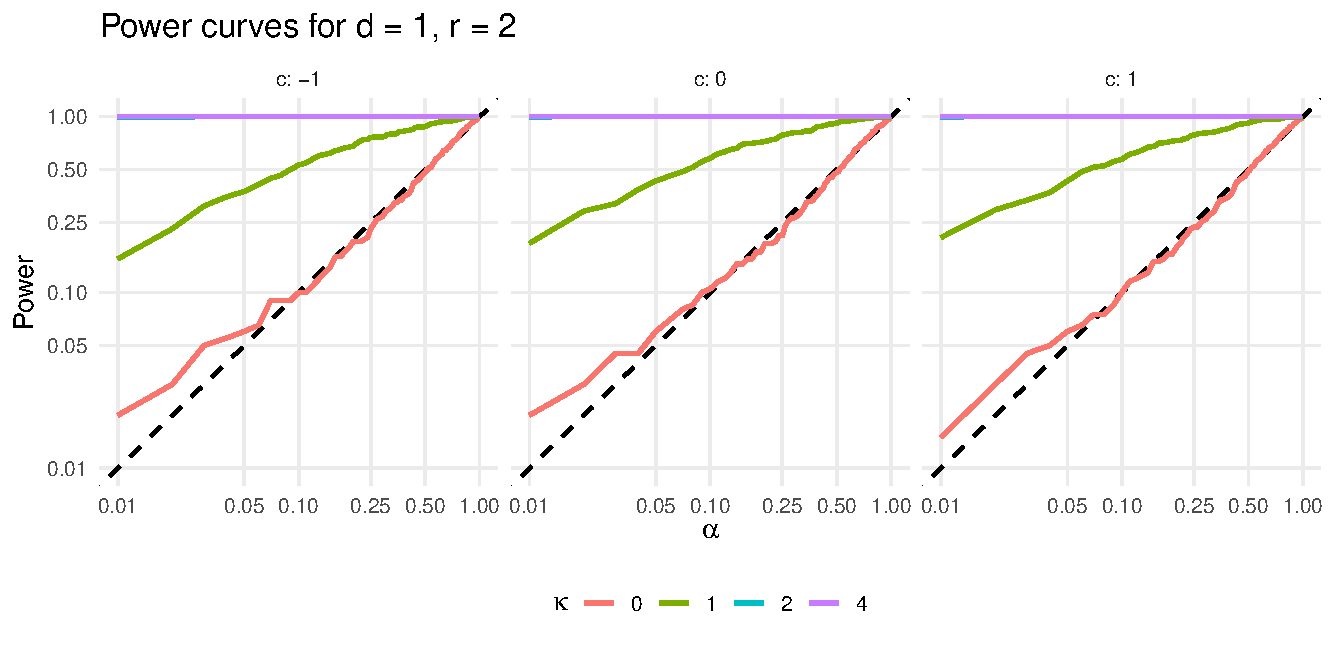
\includegraphics[width=0.85\linewidth]{plots/power_curve_1.pdf}
    \caption{Empirical power as a function of the significance level in the model ``Mixture of iid von Mises--Fisher distributions'', for $n=100$, $d=1$ and $r=2$; the parameter $\kappa \in [0,\infty)$ represents deviation from independence, and $c = -1, 0, 1$ is a tuning parameter related to the degree of smoothness (see the text in this section). Axes in log-scale.} 
    \label{fig:powercurve1}
\end{figure}

\begin{figure}[H]
    \centering
    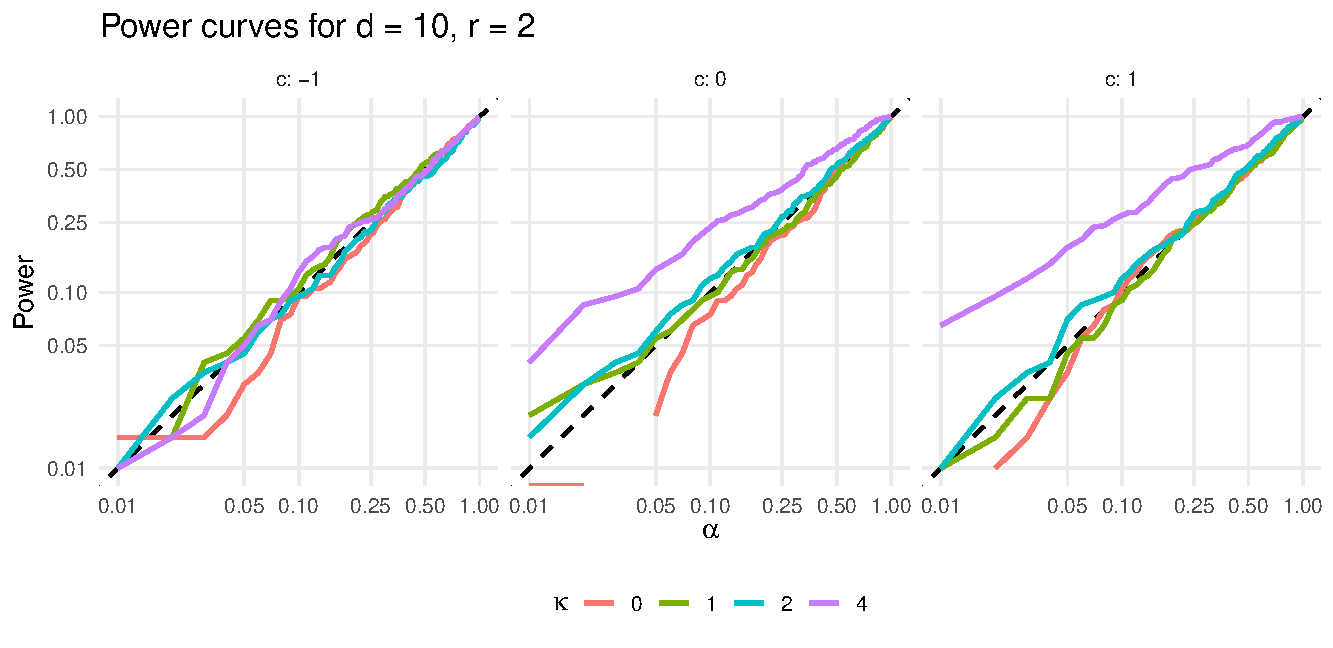
\includegraphics[width=0.85\linewidth]{plots/power_curve_2.pdf}
    \caption{Same description as in Figure \ref{fig:powercurve1}, but with $d=10$ and $r=2$.} 
    \label{fig:powercurve2}
\end{figure}

\begin{figure}[H]
    \centering
    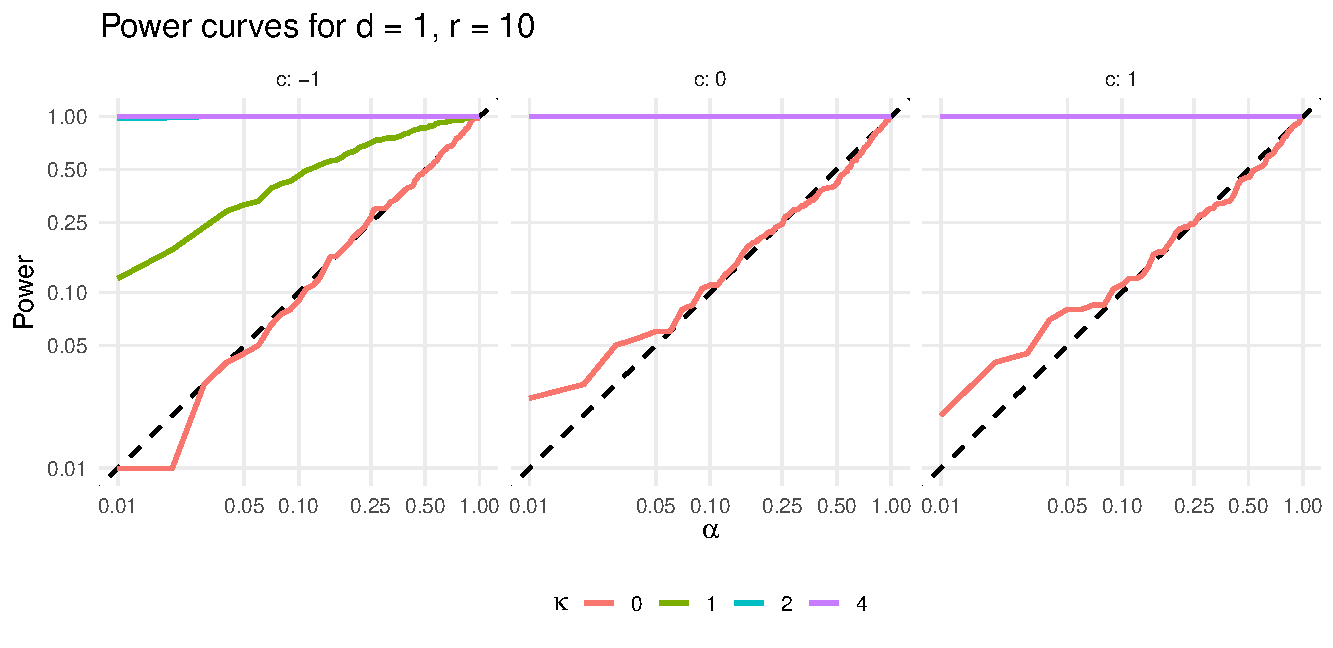
\includegraphics[width=0.85\linewidth]{plots/power_curve_3.pdf}
    \caption{Same description as in Figure \ref{fig:powercurve1}, but with $d=1$ and $r=10$.} 
    \label{fig:powercurve3}
\end{figure}

%Tables with additional results from the simulation study, showing the empirical power for different combination of parameters $d,r,n,a,c$ under a $\alpha = 0.05$ significance level, are available in Section \ref{sec:simultation_tables} in Appendix. As a general pattern, the power increased as a function of both the sample size $n$ and the dependence parameter $a$, which is coherent with the theory previously developed in this paper. The test performance was severally affected by the dimension $d$ of the hyperspheres.

%-------------------------------%
\section{Real data applications}
\label{sec:realdata}
%-------------------------------%

\subsection{Serial dependence in comet records}

A possible application of the testing procedure developed in this paper is to identify the existence of serial dependence in a sequence of records of a directional variable. Here we consider an astronomical dataset already discussed in \cite{Garcia-Portugues2024b}, which consists of a sequence of records of directions obtained from comet positions - for details concerning the data and its astronomic interpretation, refer to \cite{Garcia-Portugues2024b}. An interesting question concerning this dataset is to verify whether there is evidence of dependence in the sequence of observations.

More specifically, we have a sequence $\{ \bX_i \}_{i = 1, \dots, 623}$ of points $\bX_i \in \mathbb{S}^{2}$ and we are interested in detecting the existence of lag-1 dependence, that is, dependence between pairs $(\bX_i, \bX_{i+1})$. To achieve this goal, we define the sample $\bZ_1, \dots, \bZ_{622}$, where
\begin{align*}
    \bZ_i \defin (\bZ_i^{(1)}, \bZ_i^{(2)}) \in \mathbb{S}^{2} \times \mathbb{S}^{2},
\end{align*}
$\bZ_i^{(1)} \defin \bX_i$ and $\bZ_i^{(2)} \defin \bX_{i+1}$. Under this notation, the null hypothesis becomes
\begin{align*}
    H_0: \bZ^{(1)} \independent \bZ^{(2)},
\end{align*}
and a rejection of this hypothesis would indicate that the comets directions records are dependent, due to either observational bias or another scientific reason.

A straightforward approach to obtain a final p-value consists of applying the permutation calibration described in Section \ref{sec-permutation} directly to the pairs $\{\bZ_i\}_{i=1, \dots, 622}$, ignoring the serial structure of the original data. In a similar way to the approach employed in the simulation study, we employed here bandwidths on the form $2^c \times h^*$, where $h^*$ is the bandwidth chosen by Least Squares Cross-Validation (see \cite{chacon2026blessingdimensionalitycrossvalidatedbandwidth}) - this allows to see the p-values as a function of the tuning parameter $c$. Under this naive strategy, the resulting p-values for the test statistic are shown in Figure \ref{fig:pvalue_comet}.

\begin{figure}[h]
\centering
        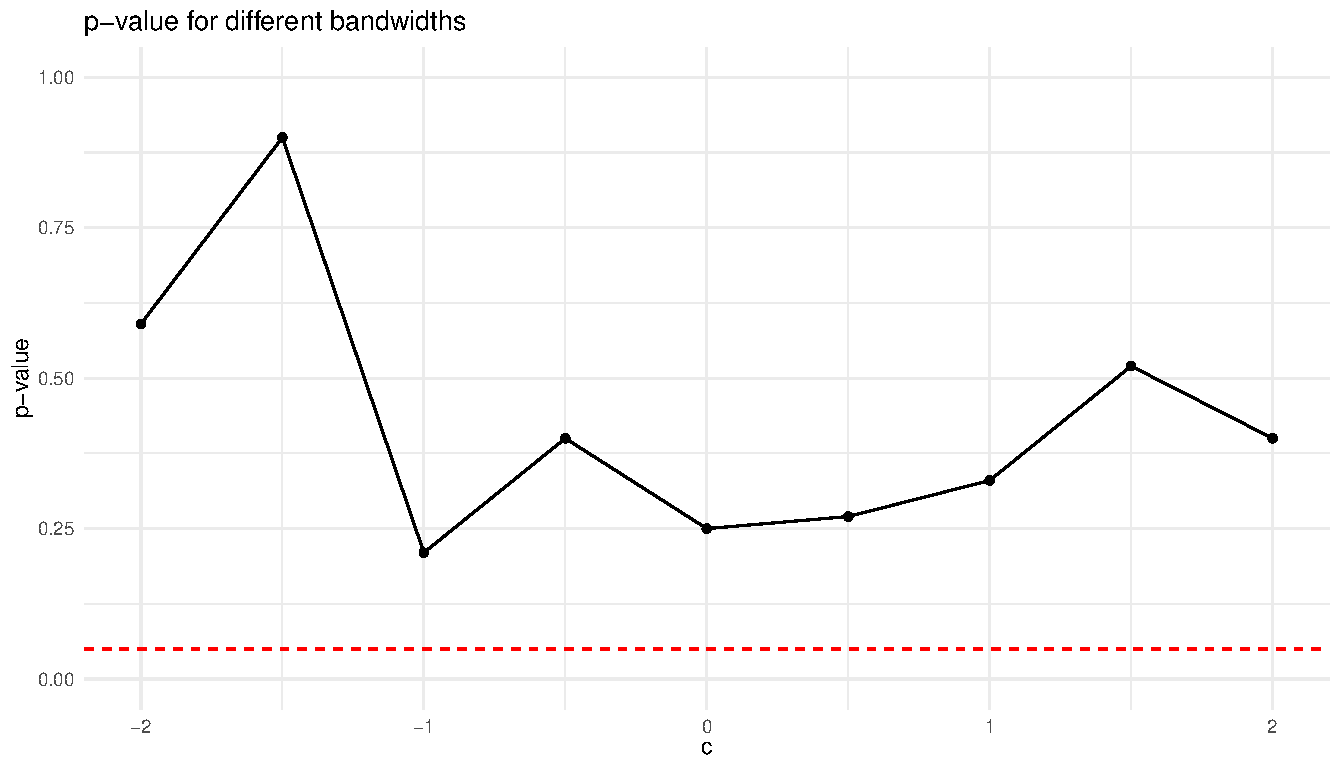
\includegraphics[totalheight=8cm]{Rplot28.pdf}
    \caption{Independence test p-value for comet records data using different combinations of bandwidths, under the standard permutation approach. The dashed red line represents the 0.05 significance level.}
    \label{fig:pvalue_comet}
\end{figure}

It must be noted, however, that the constructed pairs $\bZ_i$ are not independent, since consecutive pairs share one common observation. As a consequence, the permutation invariance assumptions required for the theoretical validity of the test are not satisfied. A detailed discussion of this issue is provided in Section \ref{app:permutation_serial} of appendix.

In order to take into account the serial structure in the definition of the $\bZ_i$'s, a different sample $\bZ'_1, \dots, \bZ'_{311}$ were defined, where
\begin{align*}
    \bZ'_i \defin (\bZ'_i^{(1)}, \bZ'_i^{(2)}) \in \mathbb{S}^{2} \times \mathbb{S}^{2},
\end{align*}
$\bZ'_i^{(1)} \defin \bX_{2i-1}$ and $\bZ'_i^{(2)} \defin \bX_{2i}$. Despite the smaller sample size, this sample would avoid the theoretical problems present in the previous approach - see Section \ref{sec-permutation}. The null hypothesis becomes again
\begin{align*}
    H_0: \bZ^{(1)} \independent \bZ^{(2)},
\end{align*}
and the obtained p-values are shown in Figure \ref{fig:pvalue_comet_step}.

\begin{figure}[h]
\centering
        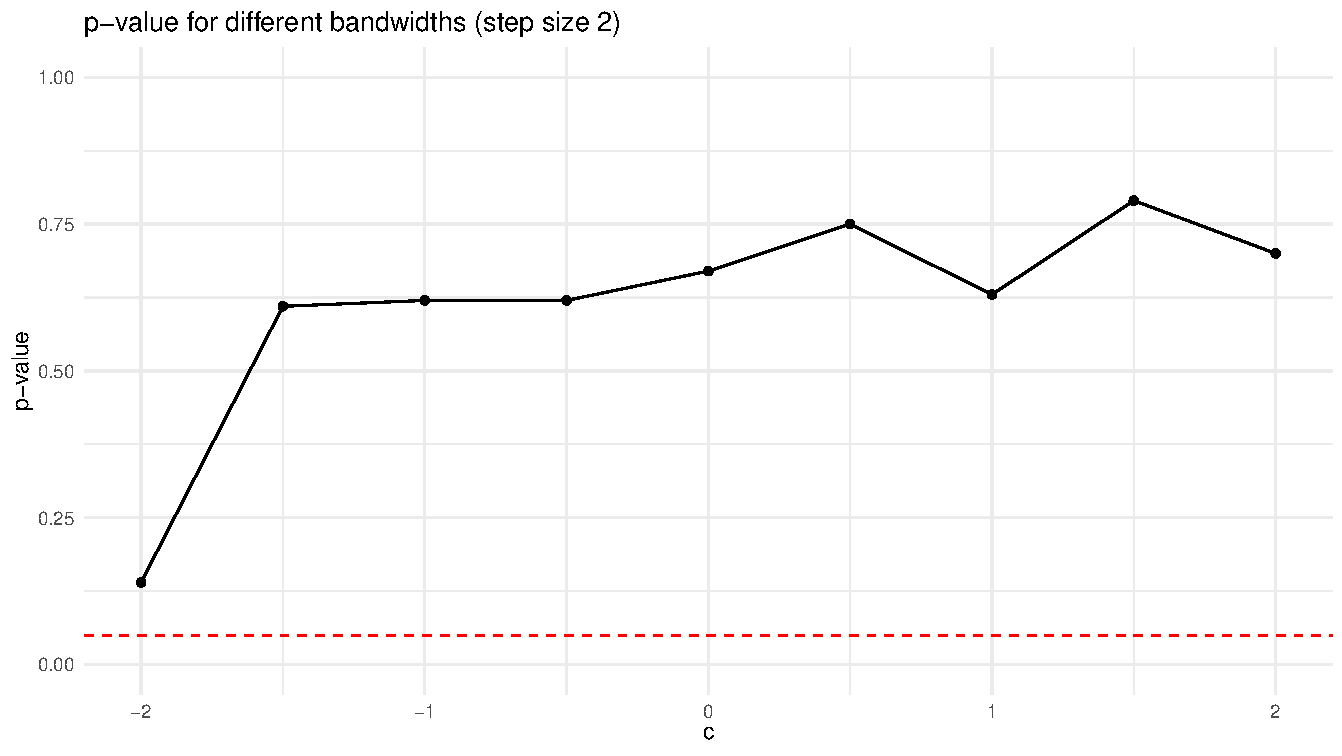
\includegraphics[totalheight=8cm]{Rplot27.pdf}
    \caption{Same description as in Figure \ref{fig:pvalue_comet}, but with step size 2.}
    \label{fig:pvalue_comet_step}
\end{figure}

Using the standard permutation approach, under a 0.05 significance level, no combination of bandwidths - among the considered ones - leads us to the rejection of the null hypothesis of independence. When the second permutation approach (with step size 2) is employed, the resulting p-values also do not allow the rejection of the null hypothesis under that significance level. Those results allow to conclude in a reasonable way that there is no evidence of serial dependence in the comet records - at least a serial dependence expressed as a lag-1 dependence.

\subsection{Dependence between regions of a hippocampus}

Previous works in the literature have successfully employed Skeletal representations (s-reps) to model the surface of hippocampi \citep{Garcia-Portugues2023hippocampus, Garcia-Portugues2024}. These models are constructed using points describing the interior of the studied object and vectors going from the interior points to the surface. The vectors describing the surface of a hippocampus, when normalized, belong to the hypersphere. Therefore, the test constructed in this text has a natural application in assessing the independence between the normalized vectors describing the hippocampi surfaces.

Here we consider the hippocampus data available in \cite{polykde}. We use the hippocampi data of the 34 autistic people present in the dataset, each of them having a hippocampus surface described by 168 random vectors $\bX^{(1)}, \dots, \bX^{(168)} \in (\mathbb{S}^{2})^{168}$. We focus our analysis in the vectors 88, 122, 146,
and 157, because they are located in different parts of the hippocampus. For each of these four vectors, we test the pairwise independence between it and each of the other 167 vectors. The results are summarized in Figure \ref{fig:pvalueshippo}.

\begin{figure}[h]
    \centering
    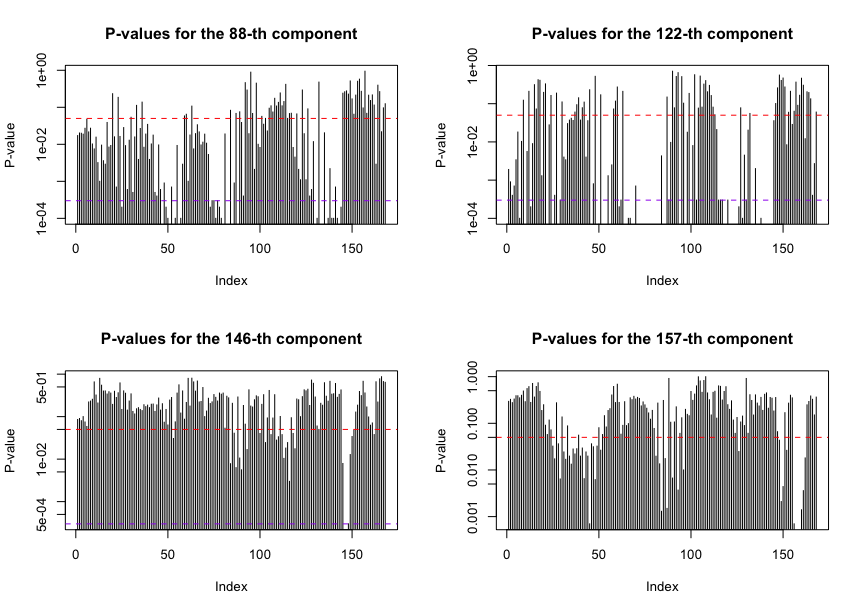
\includegraphics[width=0.75\linewidth]{Rplot13.png}
    \caption{P-values for pairwise independence test between each mentioned vector (88, 122, 146, 157) and each of the other 167 vectors. Red line represents 0.05 significance level, and the purple line represent the significance level corrected by Bonferroni. Y-axis in log-scale.}
    \label{fig:pvalueshippo}
\end{figure}

%Using Bonferroni's correction, 28 vectors (25, 47, 49, 50, 51, 53, 54, 56, 57, 73, 76, 78, 79, 80, 82, 83, 85 , 130, 131, 133, 134, 136, 137, 139, 140, 142, 143, 144) showed significant dependence with the 88th one; 57 vectors (7, 10, 13, 22, 25, 28, 46, 49, 50, 52, 53, 54, 56, 61, 64, 65, 66, 67, 68, 69, 71, 72, 73, 74, 75, 76, 77, 78, 79, 80, 81, 82, 83, 85, 86, 94, 97, 100, 118, 119, 121, 123, 124, 125, 126, 128, 133, 134, 136, 137, 138, 139, 140, 141, 142, 143, 144) showed significant dependence with the 122th one; one vector (147) showed significant dependence with the 146th one; and, finally, two vectors (158, 159) showed significant dependence with the 157th one.
Using Bonferroni's correction and adopting 0.05 as the original significance level, 28 vectors (25, 47, 49-51, 53, 54, 56, 57, 73, 76, 78-80, 82, 83, 85 , 130, 131, 133, 134, 136, 137, 139, 140, 142-144) showed significant dependence with the 88th one; 57 vectors (7, 10, 13, 22, 25, 28, 46, 49, 50, 52-54, 56, 61, 64-69, 71-83, 85, 86, 94, 97, 100, 118, 119, 121, 123-126, 128, 133, 134, 136-144) showed significant dependence with the 122th one; one vector (147) showed significant dependence with the 146th one; and, finally, two vectors (158, 159) showed significant dependence with the 157th one.

These findings are summarized in Figure \ref{fig:hippocampus1}, where the skeletal representation of the hippocampus of the first individual in the considered sample was plotted, and, for each vector under consideration (88, 122, 146,
and 157), it was shown the vectors those dependence with it is statistically significant. Informally, the plotted results suggest a kind of spatial pattern in the dependence structure, with vectors significantly dependent with a same reference vector being close to each other; also, in all the fours cases, they show some closeness to the reference vector; this enables conjecturing interesting neuroscientific hypotheses concerning the way that hippocampi are formed.

\begin{figure}[h]
\centering

\begin{subfigure}{0.45\linewidth}
\centering
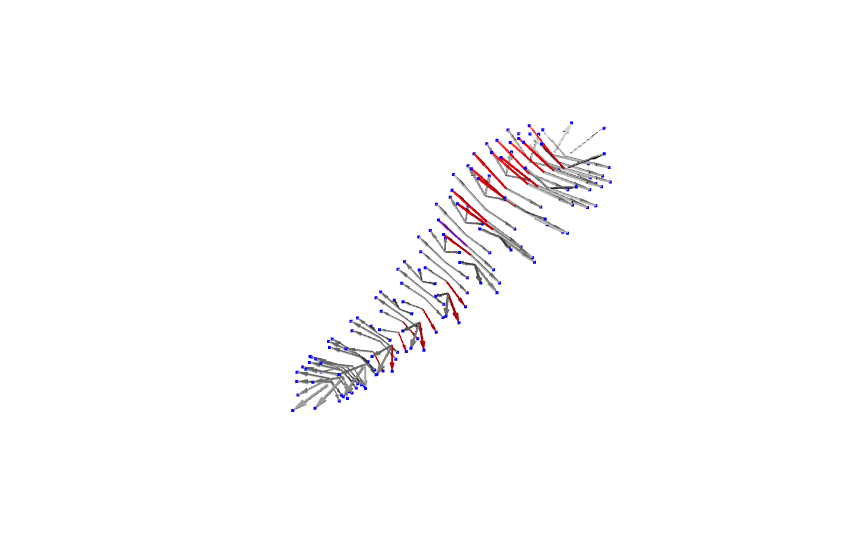
\includegraphics[width=\linewidth]{hippocampus88.png}
\caption{Case 88}
\end{subfigure}
\hfill
\begin{subfigure}{0.45\linewidth}
\centering
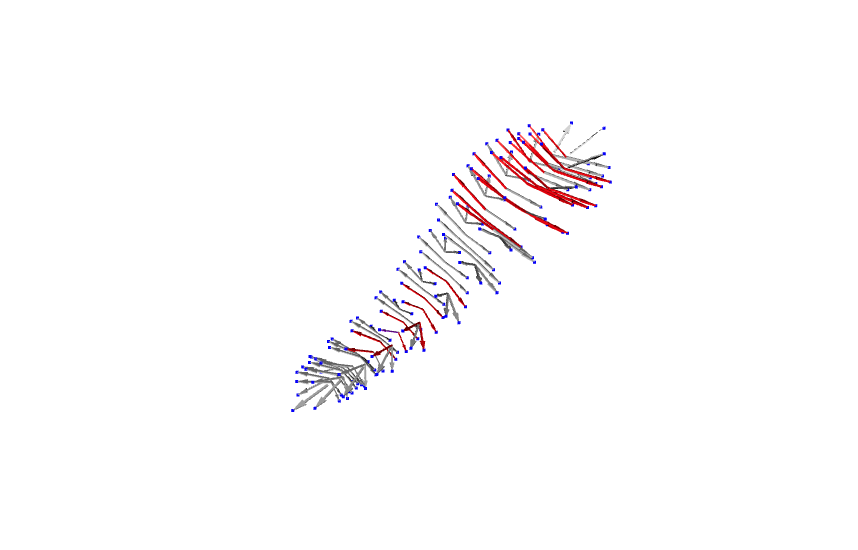
\includegraphics[width=\linewidth]{hippocampus122.png}
\caption{Case 122}
\end{subfigure}

\vspace{0.4cm}

\begin{subfigure}{0.45\linewidth}
\centering
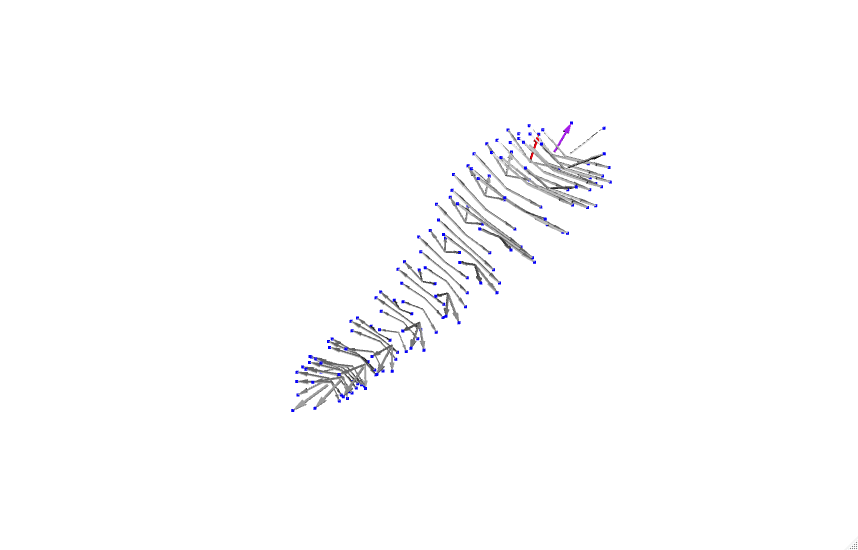
\includegraphics[width=\linewidth]{hippocampus146.png}
\caption{Case 146}
\end{subfigure}
\hfill
\begin{subfigure}{0.45\linewidth}
\centering
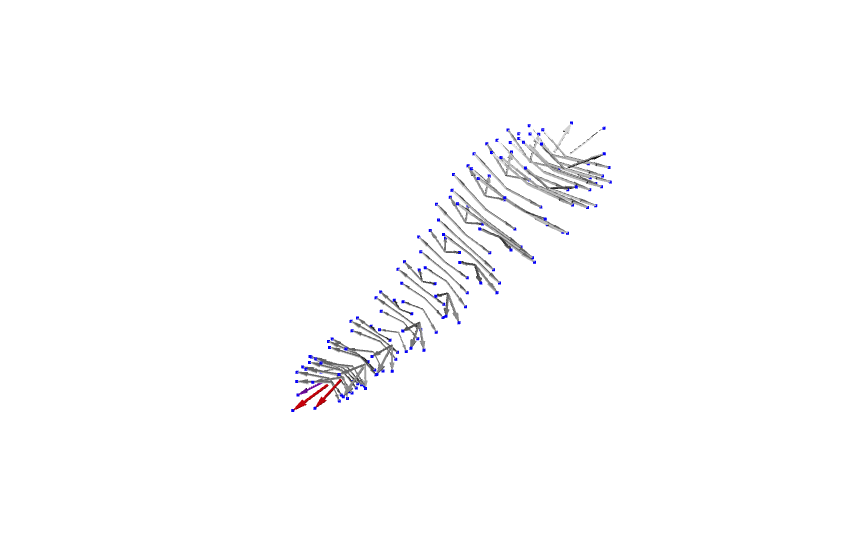
\includegraphics[width=\linewidth]{hippocampus157.png}
\caption{Case 157}
\end{subfigure}

\caption{Visualization of the hippocampus shape of the first autistic individual in the dataset. The purple arrow (88, 122, 146,
and 157) represents the vector under study, and the red arrows represent the vectors whose dependence with the studied vector is statistically significant.}
\label{fig:hippocampus1}
\end{figure}

%-----------------------------------------------%
\section*{Acknowledgments}
%-----------------------------------------------%

The first and second authors acknowledge support from grant PCI2024-155058-2, funded by MICIU/AEI/10.13039/\-501100011033/UE. The third author is funded by the Deutsche Forschungsgemeinschaft (DFG, German Research Foundation), grant 541565572. 

\appendix

%-------------------------------%
\section{Proofs of the results}
\label{sec:proofs}
%-------------------------------%

%

\begin{proof}[\textcolor{red}{[Almost completely proved, but we need to prove the asymptotics of $\mathsf{E}(G_n^2)$]} Proof of Lemma \ref{lemma-in1}]
    We have the following calculations:
    \begin{align*}
    T_{n,1} &= \int_{\Sr} \Bigg[ \frac{1}{n} \sum_{i=1}^{n} L_{\bh} (\bx,\bX_i) - \mathsf{E} \Big( \frac{1}{n} \sum_{i=1}^{n} L_{\bh} (\bx,\bX_i) \Big) \Bigg]^2 \,\rd \bx \\
    &= \frac{1}{n^2} \int_{\Sr} \Bigg[ \sum_{i=1}^{n} \Bigg\{ L_{\bh} (\bx,\bX_i) - \mathsf{E} \Big( L_{\bh} (\bx,\bX_i)) \Big) \Bigg\} \Bigg]^2 \,\rd \bx \\
    &= \frac{1}{n^2} \int_{\Sr} \Bigg[ \sum_{i=1}^{n} \bar{L}_{\bh} (\bx,\bX_i)  \Bigg]^2 \,\rd \bx.
\end{align*}
Therefore, $T_{n,1} = I_{n,2} + I_{n,3}$, where
\begin{align*}
    I_{n,2} &:= \frac{1}{n^2} \sum_{i=1}^{n} \int_{\Sr}  \lrb{\bar{L}_{\bh} (\bx,\bX_i)}^2\,\rd \bx; \\
    I_{n,3} &:= \frac{2}{n^2} \sum_{1 \le i<k \le n} \int_{\Sr} \bar{L}_{\bh} (\bx,\bX_i) \bar{L}_{\bh} (\bx,\bX_k) \,\rd \bx.
\end{align*}
Note that $I_{n,2}$ can be written as $I_{n,2} = \frac{1}{n^2} \sum_{i=1}^{n} Z_{ni}$, where $Z_{ni} \defin \int_{\Sr} \bar{L}_{\bh}^2 (\bx,\bX_i)  \,\rd \bx$ are independent and identically distributed terms. Using the fact that $\mathsf{Var} (\hat{f}(\bx;\bh) )=\frac{v_{\bd}(L)}{n \rho(\bh)} f(\bx)(1 + o(1))$,
\begin{align*}
    \mathsf{E} (Z_{ni}) &= \mathsf{E} \Bigg(\int_{\Sr}  \bar{L}_{\bh}^2 (\bx,\bX_i)  \,\rd \bx \Bigg) \\
    &= \int_{\Sr} \mathsf{E} (  \bar{L}_{\bh}^2 (\bx,\bX_i) ) \,\rd \bx \\
    &= \int_{\Sr} \mathsf{Var} (  L_{\bh} (\bx,\bX_i) ) \,\rd \bx \\
    &= \int_{\Sr} n \Bigg( \frac{v_{\bd}(L)}{n \rho(\bh)} f(\bx) (1+ o(1)) \Bigg) \,\rd \bx \\
    &= \frac{v_{\bd}(L)}{\rho(\bh)} \int_{\Sr} f(\bx) \,\rd \bx(1+ o(1)) \\
    &= \frac{v_{\bd}(L)}{\rho(\bh)} (1+ o(1)).
\end{align*}
%where $v_{\bd}(L) \defin \lambda_{\bd}(L^2) / \lambda_{\bd}(L)^2$ and $\lambda_{\bd}(L) \defin \omega_{\bd - 1} \int_{\R_+^r} L(s) s_j \prod_{i=1}^{r} s_j^{d_j/2 -1} \mathsf{d}s$.
Therefore,
\begin{align*}
    \mathsf{E} (I_{n,2}) &=  \frac{v_{\bd}(L)}{n \rho(\bh)} (1+ o(1)).
\end{align*}

Applying the $C_p$ inequality, we obtain:
\begin{align*}
    \mathsf{E} (Z_{n1}^2) =&\; \mathsf{E} \Bigg( \Bigg(\int_{\Sr}  \bar{L}_{\bh}^2 (\bx,\bX_1)  \,\rd \bx \Bigg)^2 \Bigg) \\
    \leq &\; \mathsf{E} \Bigg( \Bigg\{ 2 \Bigg(\int_{\Sr}  L_{\bh}^2 (\bx,\bX_1)  \,\rd \bx + \int_{\Sr}  \mathsf{E} (L_{\bh}^2 (\bx,\bX_1))  \,\rd \bx  \Bigg) \Bigg\}^2 \Bigg) \\
    \leq &\; 8 \Bigg\{  \mathsf{E} \Bigg( \Bigg(\int_{\Sr}  L_{\bh}^2 (\bx,\bX_1)  \,\rd \bx \Bigg)^2 \Bigg) + \mathsf{E} \Bigg( \Bigg( \int_{\Sr}  \mathsf{E} (L_{\bh}^2 (\bx,\bX_1))  \,\rd \bx  \Bigg)^2 \Bigg) \Bigg\}.
\end{align*}

Using Lemma \ref{lemma-equivLh}, we obtain:
\begin{align*}
    \mathsf{E} (Z_{n1}^2) \asymp &\; 8 \Bigg\{ \mathsf{E} \Bigg( \Bigg( \frac{\lambda_{\bd}(L^2)}{\lambda_{\bd}(L)^2} \rho(\bh)^{-1} \Bigg)^2 \Bigg) + \Bigg( \int_{\Sr}  \frac{\lambda_{\bd}(L^2)}{\lambda_{\bd}(L)^2} \rho(\bh)^{-1} f(\bx) \rd \bx \Bigg)^2  \Bigg\} \\
     =&\; 8 \Bigg\{ \Bigg( \frac{\lambda_{\bd}(L^2)}{\lambda_{\bd}(L)^2} \Bigg)^2 \rho(\bh)^{-2} + \Bigg( \frac{\lambda_{\bd}(L^2)}{\lambda_{\bd}(L)^2} \Bigg)^2 \rho(\bh)^{-2}  \Bigg\} \\
     =&\; 16 \Bigg( \frac{\lambda_{\bd}(L^2)}{\lambda_{\bd}(L)^2} \Bigg)^2 \rho(\bh)^{-2}.
\end{align*}

Note that:
\begin{align*}
    \mathsf{Var} (I_{n,2}) =&\; \mathsf{Var} \Bigg( \frac{1}{n^2} \sum_{i=1}^{n} Z_{ni} \Bigg) \\
    =&\; n^{-3} \mathsf{Var} (Z_{ni}) \\
    \leq &\; n^{-3} \mathsf{E} (Z_{ni}^2) \\
    \asymp &\; n^{-3} 16 \Bigg( \frac{\lambda_{\bd}(L^2)}{\lambda_{\bd}(L)^2} \Bigg)^2 \rho(\bh)^{-2}.
\end{align*}

As a consequence,
\begin{align*}
    \mathsf{Var} (I_{n,2}) =&\; O(n^{-3} \rho(\bh)^{-2}).
\end{align*}



%The asymptotic distribution of $T_{n,1} = I_{n,2} + I_{n,3}$ can be described through Lemma 1 in \cite{Garcia-Portugues2015}. In this case,
%\begin{align*}
 %   B_n^{-1/2} T_{n,1} \xrightarrow{d} \mathcal{N}(0, 1),
%\end{align*}
%where $B_n = n \mathsf{E} (\varphi_n^2(X_1)) + \frac{1}{2} n^2 \mathsf{E}(H_n^2(X_1,X_2))$ and $\varphi_n(X_1) = \frac{1}{n^2} \int_{\Sr} \Bigg[ \Bigg\{ \prod_{j=1}^{r} L_{\bh} (x,X_j^{(1)}) - \prod_{j=1}^{r} \mathsf{E} \Big( L_{\bh} (x,X_j^{(1)}) \Big) \Bigg\}^2 \Bigg] \,\rd \bx$.

%Using Lemma 1 in \cite{Garcia-Portugues2015} {\color{red} Need to check conditions}, it follows that:

\textit{Asymptotic behavior of $I_{n3}$.} 

Given that 
\begin{align*}
I_{n,3}=\frac{2}{n^2} \sum_{1 \le i<k \le n} \int_{\Sr} \bar{L}_{\bh} (\bx,\bX_i) \bar{L}_{\bh} (\bx,\bX_k) \,\rd \bx\defin\sum_{1 \le i<k \le n} H_n(\bX_i,\bX_k)
\end{align*}
%is a degenerate $U$-statistic, we can apply Theorem 1 in \cite{hall1984central}, which states that, if we define $H_n$ as being the kernel of the $U$-statistic; $G_n(\bx,\by) \defin \mathsf{E} (H_n(\bX_1,\bx)H_n(\bX_1,\by))$; and, further, $A_n \defin n^3 \mathsf{E} (H_n^4(\bX_1, \bX_2)) + n^4 \mathsf{E} (G_n^2(\bX_1,\bX_2))$ and $B_n \defin n^2 \mathsf{E}(H_n^2(\bX_1,\bX_2))$; then it follows from the aforementioned theorem that, if $A_n / B_n^2 \to 0$, then
is a degenerate $U$-statistic, we can apply Theorem 1 in \cite{hall1984central}, which states that, if we define $H_n$ as being the kernel of the $U$-statistic; $G_n(\bx,\by) \defin \mathsf{E} (H_n(\bX_1,\bx)H_n(\bX_1,\by))$; and, further, $A_n \defin n^{-1} \mathsf{E} (H_n^4(\bX_1, \bX_2)) + \mathsf{E} (G_n^2(\bX_1,\bX_2))$ and $B_n \defin \mathsf{E}(H_n^2(\bX_1,\bX_2))$; then it follows from the aforementioned theorem that, if $A_n / B_n^2 \to 0$, then
    \begin{align*}
        B_n^{-1/2} I_{n,3} \xrightarrow{d} \mathcal{N}(0, 1),
    \end{align*}
where $B_n = \frac{2}{n^2} \int_{\Sr} \int_{\Sr} \mathsf{E}^2 ( \bar{L}_{\bh} (\bx,\bX_1) \bar{L}_{\bh} (\by,\bX_1) ) \,\rd \bx \,\rd \by$.

Observe that the ratio $A_n/B_n^2$ is invariant to constants in the kernel $H_n$. Hence, the ratio behaves equally for $H_n(\bX_1,\bX_2)$ than for
\begin{align*}
    \tilde{H}_n(\bX_1, \bX_2) \defin \int_{\Sr} \bar{L}_{\bh} (\bx,\bX_1) \bar{L}_{\bh} (\bx,\bX_2) \,\rd \bx.
\end{align*}
We study the asymptotic behavior of the ratio for the latter expression.

\textit{Asymptotic behavior of $\mathsf{E} (\tilde{H}_n^4(\bX_1, \bX_k))$.} 

We now consider the following calculations:
\begin{align*}
    \mathsf{E} ( \tilde{H}_n^4(\bX_1, \bX_2)) &= \mathsf{E}\lrb{ \lrb{\int_{\Sr} \bar{L}_{\bh} (\bx,\bX_1) \bar{L}_{\bh} (\bx,\bX_2) \,\rd \bx}^4 } \\
    &= \mathsf{E}\lrb{ \prod_{k=1}^{4} \lrb{\int_{\Sr} \bar{L}_{\bh} (\bx_k,\bX_1) \bar{L}_{\bh} (\bx_k,\bX_2) \,\rd \bx_k} } \\ 
    &= \mathsf{E} \lrb{\int_{(\Sr)^4} \prod_{k=1}^{4}\bar{L}_{\bh} (\bx_k,\bX_1) \bar{L}_{\bh} (\bx_k,\bX_2) \prod_{k=1}^{4} \,\rd \bx_k}  \\
    &= \int_{(\Sr)^4} \mathsf{E} \lrb{ \prod_{k=1}^{4}\bar{L}_{\bh} (\bx_k,\bX_1) \bar{L}_{\bh} (\bx_k,\bX_2) }\prod_{k=1}^{4} \,\rd \bx_k  \\
    &= \int_{(\Sr)^4} \mathsf{E} \lrb{ \prod_{k=1}^{4}\bar{L}_{\bh} (\bx_k,\bX_1)} \mathsf{E} \lrb{ \prod_{k=1}^{4} \bar{L}_{\bh} (\bx_k,\bX_2) }\prod_{k=1}^{4} \,\rd \bx_k  \\
    &= \int_{(\Sr)^4} \mathsf{E}^2 \lrb{ \prod_{k=1}^{4}\bar{L}_{\bh} (\bx_k,\bX_1)} \prod_{k=1}^{4} \,\rd \bx_k.
\end{align*}

Now note that
\begin{align*}
    \mathsf{E} \lrb{ \prod_{k=1}^{4}\bar{L}_{\bh} (\bx_k,\bX_1)} =&\; \mathsf{E} \lrb{ \prod_{k=1}^{4} \lrb{ L_{\bh} (\bx_k,\bX_1) - \mathsf{E} (L_{\bh} (\bx_k,\bX_1)) } } \\
    =&\; \mathsf{E} \lrb{ L_{\bh} (\bx_1,\bX_1) L_{\bh} (\bx_2,\bX_1) L_{\bh} (\bx_3,\bX_1) L_{\bh} (\bx_4,\bX_1)}  \\
    &- \mathsf{E} \lrb{ L_{\bh} (\bx_1,\bX_1) L_{\bh} (\bx_2,\bX_1) L_{\bh} (\bx_3,\bX_1) \mathsf{E} (L_{\bh} (\bx_4,\bX_1))} \\
    &+ \cdots
\end{align*}
From the $C_p$ inequality, it follows that the dominant terms of $\mathsf{E}^2 \lrb{ \prod_{k=1}^{4}\bar{L}_{\bh} (\bx_k,\bX_1)}$ will be the squares of the expectations of the terms in the decomposition above.

If we consider the first term, we have
\begin{align*}
    t_1 &\defin \int_{(\Sr)^4} \mathsf{E}^2 \lrb{ L_{\bh} (\bx_1,\bX_1) L_{\bh} (\bx_2,\bX_1) L_{\bh} (\bx_3,\bX_1) L_{\bh} (\bx_4,\bX_1)} \prod_{k=1}^{4} \,\rd \bx_k \\
    &= \int_{(\Sr)^4} \lrb{ \int_{\Sr}L_{\bh} (\bx_1,\by) L_{\bh} (\bx_2,\by) L_{\bh} (\bx_3,\by) L_{\bh} (\bx_4,\by) f(\by) \,\rd \by }^2 \prod_{k=1}^{4} \,\rd \bx_k.
\end{align*}

Now let's apply Lemma \ref{lemma-tnd-poly} on $t_1$. To simplify the notation, consider $J_k(\bs_k) \defin \prod_{j=1}^r \lrb{1 - (\bs_k^{(j)})^2}^{d_j/2 -1}$ for $\bs_k\in[-1,1]^r$. Applying the tangent-normal decomposition in the variables $\bx_2,\bx_3,\bx_4$ in $t_1$, as described in Lemma \ref{lemma-tnd-poly}, we obtain
\begin{align*}
    t_1 =&\; \int_{\Sr} \int_{([-1,1]^r)^3} \int_{(\Srm)^3} \lrb{ \int_{\Sr}L_{\bh} (\bx_1,\by) \prod_{k=2}^{4} c_{\bd,L}(\bh) L \lrb{ \frac{1 - s_k}{\bh^{\odot 2 }} } f(\by) \,\rd \by }^2 \prod_{k=2}^{4} J_k(\bs_k) \,\rd \bxi \,\rd s \,\rd \bx_1.
\end{align*}
We can apply again the tangent-normal decomposition, this time on $\by^{(j)}$: $\by_k^{(j)} = s_k^{(j)} \bx_1^{(j)} + \lrb{1 - \lrb{s_k^{(j)}}^2}^{1/2} B_{x_1^{(j)}} \bxi_1^{(j)}$, for $j \in \{ 1, \dots, r \}$. This leads us to
\begin{align*}
    t_1 =&\; [c_{\bd,L}(\bh)]^8 \int_{\Sr} \int_{([-1,1]^r)^3} \int_{(\Srm)^3} \lrb{ \int_{[-1,1]^r} \int_{\Sr} \prod_{k=1}^{4} L \lrb{ \frac{1 - s_k}{\bh^{\odot 2 }} } f \{ s_1^{(j)} \bx_1^{(j)} + \lrb{1 - \lrb{s_1}^2}^{1/2} B_{x_1} \bxi_1 } \\
    & \,\rd \bxi_1 J_1(s_1) \,\rd s_1 \}^2 \prod_{k=2}^{4} J_k(s_k) \,\rd \bxi \,\rd s \,\rd \bx_1.
\end{align*}

Now consider the transformation $t_k^{(j)} = \frac{1 - s_k^{(j)}}{h_j^2}$. Therefore, $\,\rd s_k^{(j)} = (-h_j^2) \,\rd t_k^{(j)}$ and, therefore,
\begin{align*}
    t_1 =&\; [c_{\bd,L}(\bh)]^8 \int_{\Sr} \int_{I_h} \int_{(\Srm)^3} \Bigg\{ \int_{[-1,1]^r} \int_{\Sr} \prod_{k=1}^{4} L \lrb{ t_k} f \lrb{ x_1 + \alpha_{x_1,\bxi_1,h} } \rho (\bh) \prod_{j=1}^r (t_1^{(j)})^{d_j/2 -1} (2 -h_j^2 t_1^{(j)})^{d_j/2 -1} \\
    & \,\rd \bxi_1 \,\rd t_1 \}^2 \prod_{k=2}^{4} J_k(t_k) \rho (\bh)^3 \,\rd \bxi \,\rd s \,\rd \bx_1 \\
    =&\; [c_{\bd,L}(\bh)]^8 \rho (\bh)^5 \omega_{\bd - 1}^3 \prod_{k=2}^4 \int_{I_h} L^4(t) J(t) \,\rd t \int_{\Sr} \lrb{ \int_{I_h} \int_{\Srm} L(t_1)  f \lrb{ x_1 + \alpha_{x_1,\bxi_1,h} } J_1(t_1) \,\rd \bxi_1 \,\rd t_1 }^2 \,\rd x_1.
\end{align*}
where $I_h \defin \times_{j=1}^r [0, 2h_j^{-2}]$.
¢£
Therefore, $t_1 = O([c_{\bd,L}(\bh)]^8 \rho (\bh)^5)$. Now remember that $c_{\bd,L}(\bh)^{-1} = \rho(\bh) \lambda_{\bh,\bd}(L)$, and, as a consequence, $c_{\bd,L}(\bh) \asymp \rho(\bh)^{-1}$. Therefore,
\begin{align*}
    t_1 &= O(\rho (\bh)^{-8} \rho (\bh)^5) \\
    &= O(\rho (\bh)^{-3}).
\end{align*}

The same arguments employed in $t_1$ can be applied in an analogous way in the remaining terms.

Without loss of generality, consider the second term as being
\begin{align*}
    t_2 &\defin \int_{(\Sr)^4} \mathsf{E}^2 \lrb{ L_{\bh} (\bx_1,\bX_1) L_{\bh} (\bx_2,\bX_1) L_{\bh} (\bx_3,\bX_1) \mathsf{E} \lrb{ L_{\bh} (\bx_4,\bX_1)} }\prod_{k=1}^{4} \,\rd \bx_k \\
    &= \int_{(\Sr)^4} \mathsf{E}^2 \lrb{ L_{\bh} (\bx_4,\bX_1)} \mathsf{E}^2 \lrb{ L_{\bh} (\bx_1,\bX_1) L_{\bh} (\bx_2,\bX_1) L_{\bh} (\bx_3,\bX_1) }\prod_{k=1}^{4} \,\rd \bx_k \\
    &= \lrb{ \int_{\Sr} \mathsf{E}^2 \lrb{ L_{\bh} (\bx_4,\bX_1)} \,\rd \bx_4} \lrb{ \int_{(\Sr)^3} \mathsf{E}^2 \lrb{ L_{\bh} (\bx_1,\bX_1) L_{\bh} (\bx_2,\bX_1) L_{\bh} (\bx_3,\bX_1) }\prod_{k=1}^{3} \,\rd \bx_k } \\
    &= \lrb{ \int_{\Sr} \lrb{ \int_{\Sr} L_{\bh} (\bx_4,\by) f(\by) \,\rd \by }^2 \,\rd \bx_4} \lrb{ \int_{(\Sr)^3} \lrb{ \int_{\Sr} L_{\bh} (\bx_1,\by) L_{\bh} (\bx_2,\by) L_{\bh} (\bx_3,\by) f(\by) \,\rd \by}^2 \prod_{k=1}^{3} \,\rd \bx_k } \\
    & \indef \theta_{4} \times \theta_{123}.
    %&= \int_{(\Sr)^4} \lrb{ \int_{\Sr}L_{\bh} (\bx_1,\by) L_{\bh} (\bx_2,\by) L_{\bh} (\bx_3,\by) L_{\bh} (\bx_4,\by) f(\by) \,\rd \by }^2 \prod_{k=1}^{4} \,\rd \bx_k.
\end{align*}
Now, note that we can apply on both $\theta_{4}$ and $\theta_{123}$ calculations analogous to the calculations done from $t_1$. Let's consider $\theta_{123}$ first; applying tangent-normal transformation of variables, we obtain
\begin{align*}
    \theta_{123} &= \int_{\Sr} \int_{([-1,1]^r)^2} \int_{(\Srm)^2} \lrb{ \int_{\Sr}L_{\bh} (\bx_1,\by) c_{\bd,L}(\bh)^2 L \lrb{ \frac{1 - \bs_2}{\bh^{\odot 2 }} } L \lrb{ \frac{1 - \bs_3}{\bh^{\odot 2 }} } f(\by) \,\rd \by }^2 J_2(\bs_2) J_3(\bs_3) \\
    & \,\rd \bxi_2 \,\rd \bxi_3 \,\rd \bs_2 \,\rd \bs_3 \,\rd \bx_1 \\
    &= [c_{\bd,L}(\bh)]^6 \int_{\Sr} \int_{([-1,1]^r)^2} \int_{(\Srm)^2} \lrb{ \int_{[-1,1]^r} \int_{\Sr} \prod_{k=1}^{3} L \lrb{ \frac{1 - \bs_k}{\bh^{\odot 2 }} } f \lrb{ s_1^{(j)} \bx_1^{(j)} + \lrb{1 - \lrb{s_1}^2}^{1/2} B_{x_1} \bxi_1 } \,\rd \bxi_1 J_1(s_1) \,\rd \bs_1 }^2 \\
    & J_2(s_2) J_3(s_3) \,\rd \bxi_2 \,\rd \bxi_3 \,\rd \bs_2 \,\rd \bxi \,\rd \bs_3 \,\rd \bx_1.
\end{align*}
Now applying Lemma \ref{lemma-tnd-poly}, we obtain
\begin{align*}
    \theta_{123} &= O([c_{\bd,L}(\bh)]^6 \rho (\bh)^4) \\
    &= O(\rho (\bh)^{-6} \rho (\bh)^4) \\
    &= O(\rho (\bh)^{-2}).
\end{align*}

Now see that
\begin{align*}
    \theta_4 & \defin \int_{\Sr} \mathsf{E}^2 \lrb{ L_{\bh} (\bx_4,\bX_1)} \,\rd \bx_4 \\
    &= \int_{\Sr} \lrb{f(\bx_4)+O((\bh^{\odot 2 })^{\top} \mathbf{1}_r)}^{2} \,\rd \bx_4 \\
    &= \int_{\Sr} \lrb{f^2(\bx_4)+O((\bh^{\odot 2 })^{\top} \mathbf{1}_r)} \,\rd \bx_4 \\
    &= R(f) + O((\bh^{\odot 2 })^{\top} \mathbf{1}_r) \\
    &= O(1).
\end{align*}

As a consequence,
\begin{align*}
    t_2 &= O(\rho (\bh)^{-2})O(1) \\
    &= O(\rho (\bh)^{-2}).
\end{align*}

Now, without loss of generality, consider the third term:
\begin{align*}
    t_3 &\defin \int_{(\Sr)^4} \mathsf{E}^2 \lrb{ L_{\bh} (\bx_1,\bX_1) L_{\bh} (\bx_2,\bX_1) \mathsf{E} \lrb{ L_{\bh} (\bx_3,\bX_1)} \mathsf{E} \lrb{ L_{\bh} (\bx_4,\bX_1)} }\prod_{k=1}^{4} \,\rd \bx_k \\
    &= \int_{(\Sr)^4} \mathsf{E}^2 \lrb{ L_{\bh} (\bx_1,\bX_1) L_{\bh} (\bx_2,\bX_1) } \mathsf{E}^2 \lrb{ L_{\bh} (\bx_3,\bX_1)} \mathsf{E}^2 \lrb{ L_{\bh} (\bx_4,\bX_1)} \prod_{k=1}^{4} \,\rd \bx_k \\
    &= \lrb{\int_{(\Sr)^2} \mathsf{E}^2 \lrb{ L_{\bh} (\bx_1,\bX_1) L_{\bh} (\bx_2,\bX_1) } \,\rd \bx_1 \,\rd \bx_2} \lrb{\int_{\Sr} \mathsf{E}^2 \lrb{ L_{\bh} (\bx_3,\bX_1)} \,\rd \bx_3} \lrb{\int_{\Sr} \mathsf{E}^2 \lrb{ L_{\bh} (\bx_4,\bX_1)} \,\rd \bx_4} \\
    &\indef \theta_{12} \times \theta_3 \times \theta_4
\end{align*}
An analogous argument used in $t_1$ and $t_2$ (see also Lemma \ref{lemma-tnd-poly}) leads us to 
\begin{align*}
    \theta_{12} &= O([c_{\bd,L}(\bh)]^4 \rho (\bh)^3) \\
    &= O(\rho (\bh)^{-4} \rho (\bh)^3) \\
    &= O(\rho (\bh)^{-1}).
\end{align*}
Therefore,
\begin{align*}
    t_3 &= O(\rho (\bh)^{-1})O(1)O(1) \\
    &= O(\rho(\bh)^{-1}).
\end{align*}

Consider, finally, the last term:
\begin{align*}
    t_4 &\defin \int_{(\Sr)^4} \mathsf{E}^2 \lrb{ \mathsf{E} \lrb{ L_{\bh} (\bx_1,\bX_1)} \mathsf{E} \lrb{ L_{\bh} (\bx_2,\bX_1)} \mathsf{E} \lrb{ L_{\bh} (\bx_3,\bX_1)} \mathsf{E} \lrb{ L_{\bh} (\bx_4,\bX_1)} }\prod_{k=1}^{4} \,\rd \bx_k \\
    &= \int_{(\Sr)^4} \mathsf{E}^2 \lrb{ L_{\bh} (\bx_1,\bX_1) } \mathsf{E}^2 \lrb{L_{\bh} (\bx_2,\bX_1) } \mathsf{E}^2 \lrb{ L_{\bh} (\bx_3,\bX_1)} \mathsf{E}^2 \lrb{ L_{\bh} (\bx_4,\bX_1)} \prod_{k=1}^{4} \,\rd \bx_k \\
    &= \prod_{k=1}^{4} \lrb{\int_{\Sr}  \mathsf{E}^2 \lrb{ L_{\bh} (\bx_k,\bX_1)} \,\rd \bx_k} \\
    & \indef \theta_1 \theta_2 \theta_3 \theta_4.
\end{align*}
It is straightforward to see that $\theta_1 =\theta_2= \theta_3= \theta_4=O(1)$, then
\begin{align*}
    t_4 = O(1).
\end{align*}

Given that $\rho (\bh) \to 0$, the dominant term is $O(\rho (\bh)^{-3})$, which leads us to the conclusion
\begin{align*}
    \mathsf{E} ( \tilde{H}_n^4(\bX_1, \bX_2)) = O(\rho (\bh)^{-3}).
\end{align*}

{\color{red}\textit{Asymptotic behavior of $\mathsf{E} (\tilde{G}_n^2(\bX_1,\bX_2))$.} 

Remember that
\begin{align*}
    \tilde{H}_n(\bx,\bX_1) &= \int_{\Sr} \bar{L}_{\bh} (\bt,\bx) \bar{L}_{\bh} (\bt,\bX_1) \,\rd \bt.
\end{align*}
Then
\begin{align*}
    \tilde{G}_n(\bx,\by) & \defin \mathsf{E} (\tilde{H}_n(\bx,\bX_1)\tilde{H}_n(\by,\bX_1))\\
    &=\int_{\Sr} \lrb{ \int_{\Sr} \bar{L}_{\bh} (\bt,\bx) \bar{L}_{\bh} (\bt,\bu) \,\rd \bt} \lrb{ \int_{\Sr} \bar{L}_{\bh} (\bs,\by) \bar{L}_{\bh} (\bs,\bu) \,\rd \bs} f(\bu) \,\rd \bu.
\end{align*}
Therefore,
\begin{align*}
    \mathsf{E} (\tilde{G}^2_n(\bX_1,\bX_2)) =&\; \int_{\Sr} \int_{\Sr} \lrb{ \int_{\Sr} \lrb{ \int_{\Sr} \bar{L}_{\bh} (\bt,\bx_1) \bar{L}_{\bh} (\bt,\bu) \,\rd \bt} \lrb{ \int_{\Sr} \bar{L}_{\bh} (\bs,\bx_2) \bar{L}_{\bh} (\bs,\bu) \,\rd \bs} f(\bu) \,\rd \bu }^2\\
    &\times f(\bx_1)f(\bx_2)\,\rd \bx_1 \,\rd \bx_2\\
    =&\; \int_{\Sr} \int_{\Sr} \lrb{ \int_{\Sr}\int_{\Sr} \int_{\Sr} \bar{L}_{\bh} (\bt,\bx_1) \bar{L}_{\bh} (\bt,\bu) \bar{L}_{\bh} (\bs,\bx_2) \bar{L}_{\bh} (\bs,\bu) f(\bu) \,\rd \bt \,\rd \bs \,\rd \bu }^2\\
    &\times f(\bx_1)f(\bx_2)\,\rd \bx_1 \,\rd \bx_2\\
\end{align*}

\begin{comment}
By Cauchy--Schwartz in the integrand on $\bu$,
\begin{align*}
    \mathsf{E} (\tilde{G}^2_n(\bX_1,\bX_2)) \leq&\; \int_{\Sr} \int_{\Sr} \Bigg\{\lrc{\int_{\Sr} \lrb{ \int_{\Sr} \bar{L}_{\bh} (\bt,\bx_1) \bar{L}_{\bh} (\bt,\bu_1) \,\rd \bt}^2 f(\bu_1) \,\rd \bu_1}\\
    &\times\lrc{\int_{\Sr}\lrb{\int_{\Sr} \bar{L}_{\bh} (\bs,\bx_2) \bar{L}_{\bh} (\bs,\bu_2) \,\rd \bs}^2 f(\bu_2) \,\rd \bu_2} \Bigg\}\\
    &\times f(\bx_1)f(\bx_2)\,\rd \bx_1 \,\rd \bx_2\\
    &= \lrb{\int_{\Sr} \int_{\Sr} \lrb{ \int_{\Sr} \bar{L}_{\bh} (\bt,\bx_1) \bar{L}_{\bh} (\bt,\bu_1) \,\rd \bt}^2 f(\bu_1) \,\rd \bu_1 f(\bx_1) \,\rd \bx_1}^2\\
    %
    % LEADS TO ORDER TOO BIG -- O(rho(h)^{-2})
\end{align*}
\end{comment}

Note that $ \bar{L}_{\bh} (\bt,\bx_1) \bar{L}_{\bh} (\bt,\bu) \bar{L}_{\bh} (\bs,\bx_2) \bar{L}_{\bh} (\bs,\bu)$ is split into 16 summands. Consider the first term, which is[check] the dominant one:
\begin{align}
    C_1 =&\;  \int_{\Sr} \int_{\Sr} \lrb{ \int_{\Sr}\int_{\Sr} \int_{\Sr} L_{\bh} (\bt,\bx_1) L_{\bh} (\bt,\bu) L_{\bh} (\bs,\bx_2) L_{\bh} (\bs,\bu) f(\bu) \,\rd \bt \,\rd \bs \,\rd \bu }^2\\
    &\times f(\bx_1)f(\bx_2)\,\rd \bx_1 \,\rd \bx_2.
\end{align}

\begin{comment}
\begin{align*}
    C_1 =&\; \int_{\Sr} \int_{\Sr} \lrb{ \int_{\Sr} \lrb{ \int_{\Sr} L_{\bh} (\bt,\bx_1) L_{\bh} (\bt,\bu) \,\rd \bt} \lrb{ \int_{\Sr} L_{\bh} (\bs,\bx_2) L_{\bh} (\bs,\bu) \,\rd \bs} f(\bu) \,\rd \bu }^2 \\
    &\times f(\bx_1)f(\bx_2)\,\rd \bx_1 \,\rd \bx_2.
\end{align*}
\end{comment}

Roadmap

$\bx_2=z\bx_1 + (1-z^2)^{1/2}\bB_{\bx_2}\bxi$

For the sphere for the moment

\begin{align*}
    C_1 =&\; c_{\bd,L}(\bh)^4\int_{\Sr} \int_{\Sr} \lrb{ \int_{\Sr}\int_{\Sr}\int_{\Sr} L\lrp{\frac{1-\bt^\top\bx_1}{h^2}} L_{\bh} (\bt,\bu) L\lrp{\frac{1-\bs^\top\bx_2}{h^2}} L_{\bh} (\bs,\bu) f(\bu) \,\rd \bt \,\rd \bs  \,\rd \bu }^2 \\
    &\times f(\bx_1)f(\bx_2)\,\rd \bx_1 \,\rd \bx_2\\
    =&\; c_{\bd,L}(\bh)^4 \int_{\Srm} \int_{[-1,1]^r} \int_{\Sr} \\
    &\times\lrb{ \int_{\Sr}\int_{\Sr} \int_{\Sr} L\lrp{\frac{1-\bt^\top\bx_1}{h^2}} L_{\bh}(\bt,\bu) L \Bigg(\frac{1 - z\bs^\top\bx_1 + (1-z^2)^{1/2}\bs^\top(\bB_{\bx_2}\bxi)}{h^2}\Bigg) L_{\bh} (\bs,\bu) f(\bu) \,\rd \bt \,\rd \bs \,\rd \bu }^2\\
    &\times J(\bz) f(\bx_1)f(z\bx_1 + (1-z^2)^{1/2}\bB_{\bx_2}\bxi)\,\rd \bx_1 \,\rd \bz \,\rd \bxi\\
    =&\;
\end{align*}




\begin{comment}
\textit{Asymptotic behavior of $\mathsf{E} (\tilde{G}_n^2(\bX_1,\bX_2))$.} Remember that
\begin{align*}
    \tilde{H}_n(\bx,\bX_1) &= \int_{\Sr} \bar{L}_{\bh} (\bt,\bx) \bar{L}_{\bh} (\bt,\bX_1) \,\rd \bt.
\end{align*}
Then
\begin{align*}
    \tilde{G}_n(\bx,\by) &= \mathsf{E} (\tilde{H}_n(\bX_1,\bx)\tilde{H}_n(\bX_1,\by))\\
    &=\int_{\Sr} \lrb{ \int_{\Sr} \bar{L}_{\bh} (\bt,\bx) \bar{L}_{\bh} (\bt,\bx_1) \,\rd \bt} \lrb{ \int_{\Sr} \bar{L}_{\bh} (\bs,\by) \bar{L}_{\bh} (\bs,\bx_1) \,\rd \bs} f(\bx_1) \,\rd \bx_1 \\
    &=  \int_{\Sr} \int_{\Sr} \int_{\Sr} \bar{L}_{\bh} (\bt,\bx) \bar{L}_{\bh} (\bt,\bx_1) \bar{L}_{\bh} (\bs,\by) \bar{L}_{\bh} (\bs,\bx_1) f(\bx_1) \,\rd \bx_1 \,\rd \bt \,\rd \bs \\
    &=  \int_{\Sr} \int_{\Sr} \bar{L}_{\bh} (\bt,\bx) \bar{L}_{\bh} (\bs,\by) \mathsf{E} (\bar{L}_{\bh} (\bt,\bX_1) \bar{L}_{\bh} (\bs,\bX_1)) \,\rd \bt \,\rd \bs.
\end{align*}

Note that, by Cauchy--Schwarz inequality,
\begin{align*}
    \mathsf{E} (\bar{L}_{\bh} (\bt,\bX_1) \bar{L}_{\bh} (\bs,\bX_1)) & \le \sqrt{\mathsf{E}^2 (\bar{L}_{\bh} (\bt,\bX_1)) \mathsf{E}^2 (\bar{L}_{\bh} (\bs,\bX_1))} \\
    &= \sqrt{\mathsf{Var} ({L}_{\bh} (\bt,\bX_1)) \mathsf{Var} ({L}_{\bh} (\bs,\bX_1))}.
\end{align*}

Therefore,
\begin{align*}
    \tilde{G}_n(\bx,\by) & \le  \int_{(\Sr)^2}  \bar{L}_{\bh} (\bt,\bx) \bar{L}_{\bh} (\bs,\by) \sqrt{\mathsf{Var} ({L}_{\bh} (\bt,\bX_1)) \mathsf{Var} ({L}_{\bh} (\bs,\bX_1))} \,\rd \bt \,\rd \bs. \\
    \tilde{G}_n^2(\bx,\by) & \le \int_{(\Sr)^4} \bar{L}_{\bh} (\bt_1,\bx) \bar{L}_{\bh} (\bt_2,\by) \bar{L}_{\bh} (\bt_3,\bx) \bar{L}_{\bh} (\bt_4,\by) \sqrt{\prod_{i=1}^{4} \mathsf{Var} ({L}_{\bh} (\bt_i,\bX_1)) } \prod_{i=1}^{4} \,\rd \bt_i.
\end{align*}

Therefore,
\begin{align*}
    \mathsf{E} (\tilde{G}_n^2(\bX_1,\bX_2)) & \le  \int_{(\Sr)^4} \mathsf{E} \lrb{ \bar{L}_{\bh} (\bt_1,\bX_1) \bar{L}_{\bh} (\bt_2,\bX_2) \bar{L}_{\bh} (\bt_3,\bX_1) \bar{L}_{\bh} (\bt_4,\bX_2)} \sqrt{\prod_{i=1}^{4} \mathsf{Var} ({L}_{\bh} (\bt_i,\bX_1)) } \prod_{i=1}^{4} \,\rd \bt_i \\
    &=  \int_{(\Sr)^4} \mathsf{E} \lrb{ \bar{L}_{\bh} (\bt_1,\bX_1) \bar{L}_{\bh} (\bt_3,\bX_1) } \mathsf{E} \lrb{ \bar{L}_{\bh} (\bt_2,\bX_2) \bar{L}_{\bh} (\bt_4,\bX_2)} \sqrt{\prod_{i=1}^{4} \mathsf{Var} ({L}_{\bh} (\bt_i,\bX_1)) } \prod_{i=1}^{4} \,\rd \bt_i \\
    &=  \int_{(\Sr)^4} \mathsf{E} \lrb{ \bar{L}_{\bh} (\bt_1,\bX_1) \bar{L}_{\bh} (\bt_3,\bX_1) } \mathsf{E} \lrb{ \bar{L}_{\bh} (\bt_2,\bX_1) \bar{L}_{\bh} (\bt_4,\bX_1)} \sqrt{\prod_{i=1}^{4} \mathsf{Var} ({L}_{\bh} (\bt_i,\bX_1)) } \prod_{i=1}^{4} \,\rd \bt_i. \\
\end{align*}

Applying Cauchy--Schwartz inequality again, we obtain
\begin{align*}
    \mathsf{E} (\tilde{G}_n^2(\bX_1,\bX_2)) \le &\;  \int_{(\Sr)^4}  \sqrt{\mathsf{Var} ({L}_{\bh} (\bt_1,\bX_1)) \mathsf{Var} ({L}_{\bh} (\bt_3,\bX_1))} \sqrt{\mathsf{Var} ({L}_{\bh} (\bt_2,\bX_1)) \mathsf{Var} ({L}_{\bh} (\bt_4,\bX_1))} \\
    & \times \sqrt{\prod_{i=1}^{4} \mathsf{Var} ({L}_{\bh} (\bt_i,\bX_1)) } \prod_{i=1}^{4} \,\rd \bt_i \\
    =&\;  \int_{(\Sr)^4} \sqrt{\prod_{i=1}^{4} \mathsf{Var} ({L}_{\bh} (\bt_i,\bX_1)) } \sqrt{\prod_{i=1}^{4} \mathsf{Var} ({L}_{\bh} (\bt_i,\bX_1)) } \prod_{i=1}^{4} \,\rd \bt_i \\
    =&\;  \int_{(\Sr)^4} \prod_{i=1}^{4} \mathsf{Var} ({L}_{\bh} (\bt_i,\bX_1)) \prod_{i=1}^{4} \,\rd \bt_i \\
    =&\;  \int_{(\Sr)^4} \prod_{i=1}^{4} n \mathsf{Var} (\hat{f}(\bt_i;\bh)) \prod_{i=1}^{4} \,\rd \bt_i \\
    =&\;  \int_{(\Sr)^4} \prod_{i=1}^{4} n \lrb{\frac{v_{\bd}(L)}{n \rho(\bh)} f(\bt_i)(1 + o(1))} \prod_{i=1}^{4} \,\rd \bt_i \\
    =&\;  \int_{(\Sr)^4} \prod_{i=1}^{4} \frac{v_{\bd}(L)}{ \rho(\bh)} f(\bt_i)(1 + o(1)) \prod_{i=1}^{4} \,\rd \bt_i \\
    =&\;  \prod_{i=1}^{4} \int_{(\Sr)^4} \frac{v_{\bd}(L)}{ \rho(\bh)} f(\bt_i)(1 + o(1)) \,\rd \bt_i \\
    =&\;  \prod_{i=1}^{4} \frac{v_{\bd}(L)}{ \rho(\bh)} (1 + o(1)) \\
    =&\;  \frac{v_{\bd}^4(L)}{ \rho^4(\bh)} (1 + o(1)).
\end{align*}

As a consequence,
\begin{align*}
    \mathsf{E} (\tilde{G}_n^2(\bX_1,\bX_2)) &= O(\rho^{-4}(\bh)).
\end{align*}
\end{comment}

\textit{Asymptotic behavior of the $\mathsf{E} ( \tilde{H}_n^2(\bX_1, \bX_2))$.}

\begin{align*}
    \mathsf{E} ( \tilde{H}_n^2(\bX_1, \bX_2)) &= \mathsf{E}\lrb{ \lrb{\int_{\Sr} \bar{L}_{\bh} (\bx,\bX_1) \bar{L}_{\bh} (\bx,\bX_2) \,\rd \bx}^2 } \\
    &= \mathsf{E}\lrb{ \prod_{k=1}^{2} \lrb{\int_{\Sr} \bar{L}_{\bh} (\bx_k,\bX_1) \bar{L}_{\bh} (\bx_k,\bX_2) \,\rd \bx_k} } \\ 
    &= \mathsf{E} \lrb{\int_{(\Sr)^2} \prod_{k=1}^{2}\bar{L}_{\bh} (\bx_k,\bX_1) \bar{L}_{\bh} (\bx_k,\bX_2) \,\rd \bx_1 \,\rd \bx_2}  \\
    &= \int_{(\Sr)^2} \mathsf{E} \lrb{ \prod_{k=1}^{2}\bar{L}_{\bh} (\bx_k,\bX_1) \bar{L}_{\bh} (\bx_k,\bX_2) } \,\rd \bx_1 \,\rd \bx_2 \\
    &= \int_{(\Sr)^2} \mathsf{E} \lrb{ \prod_{k=1}^{2}\bar{L}_{\bh} (\bx_k,\bX_1)} \mathsf{E} \lrb{ \prod_{k=1}^{2} \bar{L}_{\bh} (\bx_k,\bX_2) } \,\rd \bx_1 \,\rd \bx_2  \\
    &= \int_{(\Sr)^2} \mathsf{E}^2 \lrb{ \bar{L}_{\bh} (\bx_1,\bX) \bar{L}_{\bh} (\bx_2,\bX)} \,\rd \bx_1 \,\rd \bx_2.
\end{align*}
Since $\bar{L}_{\bh} (\bx_1,\bX)=L_{\bh} (\bx_1,\bX)-\mathsf{E}\lrb{L_{\bh} (\bx_1,\bX)}$, we have
\begin{align*}
    \mathsf{E}^2 \lrb{ \bar{L}_{\bh} (\bx_1,\bX) \bar{L}_{\bh} (\bx_2,\bX)} =&\; \mathsf{E}^2 \Big\{{L}_{\bh} (\bx_1,\bX){L}_{\bh} (\bx_2,\bX) - {L}_{\bh} (\bx_1,\bX)\mathsf{E}\lrb{{L}_{\bh} (\bx_2,\bX)}\\
    &- \mathsf{E} \lrb{{L}_{\bh} (\bx_1,\bX)} {L}_{\bh} (\bx_2,\bX) +  \mathsf{E} \lrb{{L}_{\bh} (\bx_1,\bX)} \mathsf{E} \lrb{{L}_{\bh} (\bx_2,\bX)}\Big\}\\
    =&\; \Big\{\mathsf{E} \lrb{{L}_{\bh} (\bx_1,\bX){L}_{\bh} (\bx_2,\bX)} - 2\mathsf{E}\lrb{{L}_{\bh} (\bx_1,\bX)}\mathsf{E}\lrb{{L}_{\bh} (\bx_2,\bX)}\\
    &+  \mathsf{E} \lrb{{L}_{\bh} (\bx_1,\bX)} \mathsf{E} \lrb{{L}_{\bh} (\bx_2,\bX)}\Big\}^2\\
    =&\; \Big\{\mathsf{E} \lrb{{L}_{\bh} (\bx_1,\bX){L}_{\bh} (\bx_2,\bX)} - \mathsf{E}\lrb{{L}_{\bh} (\bx_1,\bX)}\mathsf{E}\lrb{{L}_{\bh} (\bx_2,\bX)}\Big\}^2.
\end{align*}
Therefore,
\begin{align*}
    \mathsf{E} ( \tilde{H}_n^2(\bX_1, \bX_2)) =&\; \int_{(\Sr)^2} \Big\{\mathsf{E} \lrb{{L}_{\bh} (\bx_1,\bX){L}_{\bh} (\bx_2,\bX)} - \mathsf{E}\lrb{{L}_{\bh} (\bx_1,\bX)}\mathsf{E}\lrb{{L}_{\bh} (\bx_2,\bX)}\Big\}^2\,\rd \bx_1 \,\rd \bx_2\\
    =&\; \int_{(\Sr)^2} \mathsf{E}^2 \lrb{{L}_{\bh} (\bx_1,\bX){L}_{\bh} (\bx_2,\bX)}\,\rd \bx_1 \,\rd \bx_2\\
    &-2\int_{(\Sr)^2} \mathsf{E} \lrb{{L}_{\bh} (\bx_1,\bX){L}_{\bh} (\bx_2,\bX)}\mathsf{E}\lrb{{L}_{\bh} (\bx_1,\bX)}\mathsf{E}\lrb{{L}_{\bh} (\bx_2,\bX)} \,\rd \bx_1 \,\rd \bx_2\\
    &+ \int_{(\Sr)^2}\mathsf{E}^2\lrb{{L}_{\bh} (\bx_1,\bX)}\mathsf{E}^2\lrb{{L}_{\bh} (\bx_2,\bX)}\,\rd \bx_1 \,\rd \bx_2\\
    \indef&\; A_1-2A_2+A_3.
\end{align*}

Note that
\begin{align*}
    A_1 =&\; \int_{(\Sr)^2} \mathsf{E}^2 \lrb{{L}_{\bh} (\bx_1,\bX){L}_{\bh} (\bx_2,\bX)}\,\rd \bx_1 \,\rd \bx_2 \\
    =&\; \int_{(\Sr)^2} \mathsf{E} \lrb{{L}_{\bh} (\bx_1,\bX_1){L}_{\bh} (\bx_2,\bX_1)} \mathsf{E} \lrb{{L}_{\bh} (\bx_1,\bX_2){L}_{\bh} (\bx_2,\bX_2)} \,\rd \bx_1 \,\rd \bx_2 \\
    =&\; \int_{(\Sr)^2} \mathsf{E} \lrb{{L}_{\bh} (\bx_1,\bX_1){L}_{\bh} (\bx_2,\bX_1) {L}_{\bh} (\bx_1,\bX_2){L}_{\bh} (\bx_2,\bX_2)} \,\rd \bx_1 \,\rd \bx_2 \\
    =&\;  \mathsf{E} \lrb{ \int_{(\Sr)^2}{L}_{\bh} (\bx_1,\bX_1){L}_{\bh} (\bx_2,\bX_1) {L}_{\bh} (\bx_1,\bX_2){L}_{\bh} (\bx_2,\bX_2) \,\rd \bx_1 \,\rd \bx_2} \\
    =&\;  \mathsf{E} \lrb{H_n^{2*} (\bX_i,\bX_k)},
\end{align*}
where $H_n^* (\bX_i,\bX_k) \defin \int_{\Sr} L_{\bh} (\bx,\bX_i) L_{\bh} (\bx,\bX_k) \,\rd \bx$.

By the assumption that we are using the product kernel  ($L_{\bh} (\bx,\by) = \prod_{j=1}^r L_{h_j} (\bx^{(j)},\by^{(j)})$),
    \begin{align*}
        H_n^* (\bX_1,\bX_2) &= \int_{\Sr} \lrb{\prod_{j=1}^r L_{h_j} (\bx^{(j)},\bX_1^{(j)})} \lrb{\prod_{k=1}^r L_{h_k} (\bx^{(k)},\bX_2^{(k)})} \,\rd \bx \\
        &= \int_{\Sr} \prod_{j=1}^r L_{h_j} (\bx^{(j)},\bX_1^{(j)}) L_{h_j}(\bx^{(j)},\bX_2^{(j)}) \,\rd \bx \\
        &= \prod_{j=1}^r \int_{\Sr} L_{h_j} (\bx^{(j)},\bX_1^{(j)}) L_{h_j}(\bx^{(j)},\bX_2^{(j)}) \,\rd \bx^{(j)} \\
        &= \prod_{j=1}^r \phi_{1_j,2_j},
    \end{align*}
    where $\phi_{i_j,l_j}$ is defined in Proof of Lemma \ref{lemma-var-tn2}. Therefore,
    \begin{align*}
        \mathsf{E}(H_n^{*2}(\bX_1,\bX_2)) &=  
        \mathsf{E} \lrb{\prod_{j=1}^r \phi_{1_j,2_j}^2} \\
        &=  \prod_{j=1}^r \mathsf{E} \lrb{ \phi_{1_j,2_j}^2} \\
        &\asymp \prod_{j=1}^r c_{d_j,L}(h_j)^4\times h_j^{3d_j} \sigma_j^2 \\
        &= c_{\bd,L}(\bh)^4 \rho(\bh)^3 \prod_{j=1}^r \sigma_j^2\\
        &\asymp  \lambda_{\bd}(L)^{-4} \rho(\bh)^{-1} \prod_{j=1}^r \sigma_j^2
    \end{align*}
    where $\sigma_j^2$ is defined in Proof of Lemma \ref{lemma-var-tn2}. Therefore, $A_1 = O(\rho(\bh)^{-1)}$

\begin{align*}
    A_2=&\;\int_{(\Sr)^2} \mathsf{E} \lrb{{L}_{\bh} (\bx_1,\bX){L}_{\bh} (\bx_2,\bX)}\mathsf{E}\lrb{{L}_{\bh} (\bx_1,\bX)}\mathsf{E}\lrb{{L}_{\bh} (\bx_2,\bX)} \,\rd \bx_1 \,\rd \bx_2 \\
    =&\; \int_{(\Sr)^2} \lrb{\int_{\Sr} {L}_{\bh} (\bx_1,\by){L}_{\bh} (\bx_2,\by) f(\by)\,\rd \by} \mathsf{E}\lrb{{L}_{\bh} (\bx_1,\bX)}\mathsf{E}\lrb{{L}_{\bh} (\bx_2,\bX)} \,\rd \bx_1 \,\rd \bx_2 \\
    =&\; \int_{(\Sr)^3} {L}_{\bh} (\bx_1,\by){L}_{\bh} (\bx_2,\by) f(\by) \mathsf{E}\lrb{{L}_{\bh} (\bx_1,\bX)}\mathsf{E}\lrb{{L}_{\bh} (\bx_2,\bX)} \,\rd \bx_1 \,\rd \bx_2 \,\rd \by \\
    =&\; \int_{\Sr} \lrb{\int_{\Sr} {L}_{\bh} (\bx_1,\by) \mathsf{E}\lrb{{L}_{\bh} (\bx_1,\bX)} \,\rd \bx_1} \lrb{\int_{\Sr} {L}_{\bh} (\bx_2,\by) \mathsf{E}\lrb{{L}_{\bh} (\bx_2,\bX)} \,\rd \bx_2}  f(\by) \,\rd \by \\
    =&\; \int_{\Sr} \lrb{\int_{\Sr} {L}_{\bh} (\bx_1,\by) \mathsf{E}\lrb{{L}_{\bh} (\bx_1,\bX)} \,\rd \bx_1}^2  f(\by) \,\rd \by \\
    =&\; \int_{\Sr} \lrb{\int_{\Sr} {L}_{\bh} (\bx_1,\by) \lrb{f(\bx_1)+O\lrb{\sum_{j=1}^{r}h_j^2}} \,\rd \bx_1}^2  f(\by) \,\rd \by \\
    =&\; \int_{\Sr} \lrb{\int_{\Sr} {L}_{\bh} (\bx_1,\by) f(\bx_1) \,\rd \bx_1 + \int_{\Sr} {L}_{\bh} (\bx_1,\by) O\lrb{\sum_{j=1}^{r}h_j^2} \,\rd \bx_1}^2  f(\by) \,\rd \by \\
    =&\; \int_{\Sr} \lrb{\lrb{f(\by)+O\lrb{\sum_{j=1}^{r}h_j^2}} + O\lrb{\sum_{j=1}^{r}h_j^2}}^2  f(\by) \,\rd \by \\
     =&\; \int_{\Sr} \lrb{f^2(\by) + O\lrb{\sum_{j=1}^{r}h_j^2}}  f(\by) \,\rd \by \\
     =&\; \int_{\Sr} f^3(\by) \,\rd \by  + O\lrb{\sum_{j=1}^{r}h_j^2} \\
     =&\; O(1).
\end{align*}

\begin{comment}
\begin{align*}
    A_2=&\;\int_{(\Sr)^2} \mathsf{E} \lrb{{L}_{\bh} (\bx_1,\bX){L}_{\bh} (\bx_2,\bX)}\mathsf{E}\lrb{{L}_{\bh} (\bx_1,\bX)}\mathsf{E}\lrb{{L}_{\bh} (\bx_2,\bX)} \,\rd \bx_1 \,\rd \bx_2\\
    =&\;\int_{(\Sr)^2} \lrb{\int_{\Sr} {L}_{\bh} (\bx_1,\by){L}_{\bh} (\bx_2,\by) f(\by)\,\rd \by}\lrb{f(\bx_1)+O\lrb{\sum_{j=1}^{r}h_j^2}}\lrb{f(\bx_2)+O\lrb{\sum_{j=1}^{r}h_j^2}} \,\rd \bx_1 \,\rd \bx_2\\
    =&\;\int_{(\Sr)^3}  {L}_{\bh} (\bx_1,\by){L}_{\bh} (\bx_2,\by) f(\by)\lrb{f(\bx_1)+O\lrb{\sum_{j=1}^{r}h_j^2}}\lrb{f(\bx_2)+O\lrb{\sum_{j=1}^{r}h_j^2}} \,\rd \bx_1 \,\rd \bx_2\,\rd \by\\
    =&\;[tangent normal decomp on \bx_1=t_1\by+... and \bx_2=t_2\by+...]
\end{align*}
\end{comment}

%\begin{align*}
%    \mathsf{E} ( \tilde{H}_n^2(\bX_1, \bX_2)) =&\; \mathsf{E}\lrb{ \lrb{\int_{\Sr} {L}_{\bh} (\bx,\bX_1) {L}_{\bh} (\bx,\bX_2) \,\rd \bx}^2 } \\
%    &- \mathsf{E}\lrb{ \lrb{\int_{\Sr} \mathsf{E}\lrb{{L}_{\bh} (\bx_1,\bX_1)} {L}_{\bh} (\bx,\bX_2) \,\rd \bx}^2 } \\
%    &- \mathsf{E}\lrb{ \lrb{\int_{\Sr} {L}_{\bh} (\bx_1,\bX_1) \mathsf{E} \lrb{{L}_{\bh} (\bx_2,\bX_1)} \,\rd \bx}^2 } \\
%    &+ \mathsf{E}\lrb{ \lrb{\int_{\Sr} \mathsf{E} \lrb{{L}_{\bh} (\bx_1,\bX_1)} \mathsf{E} \lrb{{L}_{\bh} (\bx_2,\bX_1)} \,\rd \bx}^2 }.
%\end{align*}

\begin{align*}
    A_3 &= \int_{(\Sr)^2}\mathsf{E}^2\lrb{{L}_{\bh} (\bx_1,\bX)}\mathsf{E}^2\lrb{{L}_{\bh} (\bx_2,\bX)}\,\rd \bx_1 \,\rd \bx_2\\
    &= \lrb{\int_{\Sr}\mathsf{E}^2\lrb{{L}_{\bh} (\bx_1,\bX)} \,\rd \bx_1} \lrb{\int_{\Sr} \mathsf{E}^2\lrb{{L}_{\bh} (\bx_2,\bX)} \,\rd \bx_2} \\
    &= \lrb{\int_{\Sr} \lrb{f(\bx_1)+O\lrb{\sum_{j=1}^{r}h_j^2}}^2 \,\rd \bx_1} \lrb{\int_{\Sr}  \lrb{f(\bx_2)+O\lrb{\sum_{j=1}^{r}h_j^2}}^2 \,\rd \bx_2} \\
    &= \lrb{\int_{\Sr} \lrb{f^2(\bx_1)+O\lrb{\sum_{j=1}^{r}h_j^2}} \,\rd \bx_1} \lrb{\int_{\Sr}  \lrb{f^2(\bx_2)+O\lrb{\sum_{j=1}^{r}h_j^2}} \,\rd \bx_2} \\
    &= \lrb{R(f) + O\lrb{\sum_{j=1}^{r}h_j^2}} \lrb{R(f) + O\lrb{\sum_{j=1}^{r}h_j^2}} \\
    &= R^2(f) + O\lrb{\sum_{j=1}^{r}h_j^2} \\
    &= O(1).
\end{align*}


%This expression can be represented as $\mathsf{E} ( \tilde{H}_n^2(\bX_1, \bX_2)) = \theta_{12} - \theta_{1}\theta_{2} - \theta_{1}\theta_{2} + \theta_{1}\theta_{2}$. We already know that $ \theta_{12} = O(\rho (\bh)^{-1})$ and $\theta_1 = \theta_2 = O(1)$; therefore,
Therefore, $A_1$ is the dominant term and we have the result:
\begin{align*}
    \mathsf{E} ( \tilde{H}_n^2(\bX_1, \bX_2)) = O(\rho (\bh)^{-1}).
\end{align*}
}

\textit{Asymptotic behavior of the ratio $\tilde{A}_n / \tilde{B}_n^2$.} Defining $\tilde{A}_n \defin n^{-1} \mathsf{E} (\tilde{H}_n^4(\bX_1, \bX_2)) + \mathsf{E} (\tilde{G}_n^2(\bX_1,\bX_2))$, then, from the previous results,
\begin{align*}
    \tilde{A}_n &= O(n^{-1}\rho(\bh)^{-3} + \rho(\bh)^{-2})
\end{align*}
Also
\begin{align*}
    \tilde{B}_n &\defin \mathsf{E}[\tilde{H}_n^2(\bX_1,\bX_2)]= O(\rho (\bh)^{-1}).
\end{align*}

Therefore,
\begin{align*}
    \frac{\tilde{A}_n}{\tilde{B}_n^2}=\frac{O(n^{-1}\rho(\bh)^{-3} + \rho(\bh)^{-2})}{O(\rho(\bh)^{-2})}=\alert{O((n\rho(\bh))^{-1}+1)}
\end{align*}


\begin{comment}
Note that
\begin{align*}
    \mathsf{E} ( \bar{L}_{\bh} (\bx,\bX_1) \bar{L}_{\bh} (\by,\bX_1) ) &= \mathsf{E} ( L_{\bh} (\bx,\bX_1) L_{\bh} (\by,\bX_1) ) - \mathsf{E} (L_{\bh} (\bx,\bX_1)) \mathsf{E} (L_{\bh} (\by,\bX_1)).
\end{align*}

Furthermore,
\begin{align*}
    \mathsf{E} ( L_{\bh} (\bx,\bX_1) L_{\bh} (\by,\bX_1) ) &= \int_{\Sr} L_{\bh} (\bx,\bt) L_{\bh} (\by,\bt) f(\bt) \,\rd \bt \\
    & \asymp L_{\bh} (\bx,\by) f(\by).\\
    \mathsf{E} (L_{\bh} (\bx,\bX_1)) &= \int_{\Sr} L_{\bh} (\bx,\bt) f(\bt) \,\rd \bt \\
    & \asymp f(\bx).\\
    \mathsf{E} (L_{\bh} (\by,\bX_1)) &= \int_{\Sr} L_{\bh} (\by,\bt) f(\bt) \,\rd \bt \\
    & \asymp f(\by).\\
\end{align*}

As a consequence,
\begin{align*}
    \mathsf{E}^2 ( \bar{L}_{\bh} (\bx,\bX_1) \bar{L}_{\bh} (\by,\bX_1) ) & \asymp \lrb{L_{\bh} (\bx,\by) f(\by) - f(\bx)f(\by)}^2 \\
    &= L_{\bh}^2 (\bx,\by) f^2(\by) + f^2(\bx)f^2(\by) -2L_{\bh} (\bx,\by) f(\bx) f^2(\by).
\end{align*}

Let's integrate each term.
\begin{align*}
    \int_{\Sr} \int_{\Sr} L_{\bh}^2 (\bx,\by) f^2(\by) \,\rd \by \,\rd \bx & \asymp \int_{\Sr} \frac{\lambda_{\bd}(L^2)}{\lambda_{\bd}(L)^2} \rho(\bh)^{-1} f^2(\bx) \,\rd \bx \\
    &= \frac{\lambda_{\bd}(L^2)}{\lambda_{\bd}(L)^2} \rho(\bh)^{-1} R(f). \\
    \int_{\Sr} \int_{\Sr} f^2(\bx)f^2(\by) \,\rd \by \,\rd \bx &= R^2(f). \\
    \int_{\Sr} \int_{\Sr}-2L_{\bh} (\bx,\by) f(\bx) f^2(\by) \,\rd \by \,\rd \bx & \asymp -2 \int_{\Sr} f(\bx) f^2(\bx) \,\rd \bx\\
    &= -2 \int_{\Sr}f^3(\bx) \,\rd \bx.
\end{align*}

Finally,
\begin{align*}
    B_n \asymp \frac{2}{n^2} \lrb{\frac{\lambda_{\bd}(L^2)}{\lambda_{\bd}(L)^2} \rho(\bh)^{-1} R(f) + R^2(f) -2 \int_{\Sr}f^3(\bx) \,\rd \bx}.
\end{align*}
\end{comment}

%$B_n\asymp 4 n^{-4}\rho(\bh)^{-1} \sigma^2$.



%CONTINUAR AQUI

\end{proof}

\begin{proof}[ Proof of Lemma \ref{lemma-sigma2}]
    %This comes from previous lemma. Tendras que decir que conecta con los calculos de mi paper de alguna forma parea hacerlo rapido para calcular las $\sigma_j^2$.

In the proof of Lemma \ref{lemma-in1}, we have saw that $\tilde{B}_n \defin (2n^{-2})^{-1} B_n$ can be decomposed as $A_1-2A_2+A_3$, where $A_1 \defin \int_{(\Sr)^2} \mathsf{E}^2 \lrb{{L}_{\bh} (\bx_1,\bX){L}_{\bh} (\bx_2,\bX)}\,\rd \bx_1 \,\rd \bx_2$ is the dominant term. Now, note that
\begin{align*}
    A_1 &= \int_{(\Sr)^2} \mathsf{E}^2 \lrb{ \prod_{j=1}^{r} {L}_{h_j} (\bx_1^{(j)},\bX_1^{(j)}){L}_{h_j} (\bx_2^{(j)},\bX_1^{(j)})}\,\rd \bx_1 \,\rd \bx_2 \\
    &= \int_{(\Sr)^2} \prod_{j=1}^{r} \mathsf{E}^2 \lrb{ {L}_{h_j} (\bx_1^{(j)},\bX_1^{(j)}){L}_{h_j} (\bx_2^{(j)},\bX_1^{(j)})}\,\rd \bx_1 \,\rd \bx_2 \\
    &= \prod_{j=1}^{r} \int_{(\Sr)^2} \mathsf{E}^2 \lrb{ {L}_{h_j} (\bx_1^{(j)},\bX_1^{(j)}){L}_{h_j} (\bx_2^{(j)},\bX_1^{(j)})}\,\rd \bx_1^{(j)} \,\rd \bx_2^{(j)} \\
    &= \prod_{j=1}^{r} \int_{(\Sr)^2} \lrb{\int_{\Sr} {L}_{h_j} (\bx_1^{(j)},\bz^{(j)}){L}_{h_j} (\bx_2^{(j)},\bz^{(j)}) f_j(\bz) \,\rd \bz}^2 \,\rd \bx_1^{(j)} \,\rd \bx_2^{(j)} \\
    &\defin \prod_{j=1}^{r} A_1^{(j)}.
\end{align*}

Now notice that $A_1^{(j)}$ is the directional analogous of the expression A1 in \cite{Garcia-Portugues2015}, which means that
\begin{align*}
    A_1 &= \prod_{j=1}^{r} \lambda_{d_j}(L)^{-4} \rho (\bh)^{-1} \sigma_j^2,
\end{align*}
where
\begin{align*}
    \sigma_j^2=R(f_j) \om{d_j-1}\om{d_j}^2 2^{3d_j/2-1} \int_0^\infty r^{d_j/2-1}\lrc{\int_0^\infty \rho^{d_j/2-1} L(\rho)\int_{-1}^1 (1-\theta^2)^{(d_j-3)/2}L(r+\rho-2\theta(r\rho)^{1/2})\,\rd \theta\,\rd \rho}^2\,\rd r.
\end{align*}

As a consequence,
\begin{align*}
    B_n \asymp 2 n^{-2} \rho(\bh)^{-1} \lambda_{\bd}(L)^{-4}  \prod_{j=1}^{r} \sigma_j^2.
\end{align*}

\begin{comment}
    \begin{align*}
    & R(f_j) \omega_{d_j-1} \omega_{d_j-2}^2 2^{\frac{3 d_j}{2}-1} \int_0^{\infty} r^{\frac{d_j}{2}-1} \int_{\mathbb{R}}\left[\int_{\mathbb{R}} \int_0^{\infty} \rho^{\frac{d_j}{2}-1} L_{h_j} (\rho, u)\right. \\ & \left.\times \int_{-1}^1\left(1-\theta^2\right)^{\frac{d_j-3}{2}} L_{h_j} \left(r+\rho-2 \theta(r \rho)^{\frac{1}{2}}, u+v\right) d \theta d \rho d u\right]^2 d v d r
\end{align*}
\end{comment}

\end{proof}

\begin{proof}[\textcolor{blue}{[Completed]} Proof of Lemma \ref{lemma-in2-e}]
    The proof comes from writing $\mathsf{E} (T_{n,2})$ as a function of $\mathsf{Var} (\hat{f}_{0}(\bx;\bh))$ and noticing that this variance can be written in terms of the two first moments of kernel density estimators of each density function $f_j$..
\begin{align*}
        \mathsf{E} (T_{n,3}) &= \mathsf{E} \Bigg( \int_{\Sr} \Big[ \hat{f}_{0}(\bx;\bh) - \mathsf{E} (\hat{f}_{0}(\bx;\bh)) \Big]^2 \,\rd \bx \Bigg) \\
        &= \int_{\Sr} \mathsf{E} \Bigg( \Big[ \hat{f}_{0}(\bx;\bh) - \mathsf{E} (\hat{f}_{0}(\bx;\bh)) \Big]^2 \Bigg) \,\rd \bx \\
        &= \int_{\Sr} \mathsf{Var} (\hat{f}_{0}(\bx;\bh)) \,\rd \bx \\
        &= \int_{\Sr} \mathsf{E} (\hat{f}_{0}^2(\bx;\bh)) - \mathsf{E}^2 (\hat{f}_{0}(\bx;\bh)) \,\rd \bx \\
        &= \int_{\Sr} \mathsf{E} \Bigg(\prod_{j=1}^r \hat{f}_{j}^2(x^{(j)};h_j)\Bigg) - \mathsf{E}^2 \Bigg(\prod_{j=1}^r \hat{f}_{j}(x^{(j)};h_j)\Bigg) \,\rd \bx \\
        &= \int_{\Sr} \Bigg\{ \prod_{j=1}^{r} [\mathsf{Var} (\hat{f}_j(x^{(j)};h_j)) + \mathsf{E}^2 (\hat{f}_j(x^{(j)};h_j))] - \prod_{j=1}^{r} \mathsf{E}^2 (\hat{f}_j(x^{(j)};h_j)) \Bigg\} \,\rd \bx.
    \end{align*}

Note that, if any $b_j \to 0$ and $a_j = O(1)$, then
\begin{align*}
    \prod_{j=1}^r (a_j + b_j) &= \Bigg( \prod_{j=1}^{r} a_j\Bigg) + \sum_{j=1}^{r} b_j \Bigg( \prod_{\substack{k=1\\k\neq j}}^r a_k \Bigg) + o \Bigg( \sum_{j=1}^{r} b_j \Bigg\{ \prod_{\substack{k=1\\k\neq j}}^r a_k\Bigg\}\Bigg).
\end{align*}

Therefore,
\begin{align*}
    \prod_{j=1}^r (a_j + b_j) -  \prod_{j=1}^r a_j &= \sum_{j=1}^{r} b_j \Bigg( \prod_{\substack{k=1\\k\neq j}}^r a_k \Bigg) + o \Bigg( \sum_{j=1}^{r} b_j \Bigg\{ \prod_{\substack{k=1\\k\neq j}}^r a_k \Bigg\}\Bigg).
\end{align*}

Therefore, using the fact that $\mathsf{Var} (\hat{f}_j(x^{(j)};h_j)) = O((n h_j^{d_j})^{-1})$, and taking $a_j \defin \mathsf{E}^2 (\hat{f}_k(x^{(k)};h_k))$ and $b_j \defin \mathsf{Var} (\hat{f}_j(x^{(j)};h_j))$,
\begin{align*}
     \mathsf{E} (T_{n,3}) =&\; \int_{\Sr} \Bigg\{ \Bigg[ \sum_{j=1}^{r} \mathsf{Var} (\hat{f}_j(x^{(j)};h_j)) \Bigg( \prod_{\substack{k=1\\k\neq j}}^r \mathsf{E}^2 (\hat{f}_k(x^{(k)};h_k)) \Bigg) \Bigg] \\
     & + o \Bigg( \sum_{j=1}^{r} \mathsf{Var} (\hat{f}_j(x^{(j)};h_j)) \Bigg\{ \prod_{\substack{k=1\\k\neq j}}^r \mathsf{E}^2 (\hat{f}_k(x^{(k)};h_k)) \Bigg\} \Bigg) \Bigg\} \,\rd \bx \\
     =&\; \int_{\Sr} \Bigg\{ \Bigg[ \sum_{j=1}^{r} \mathsf{Var} (\hat{f}_j(x^{(j)};h_j)) \Bigg( \prod_{\substack{k=1\\k\neq j}}^r \mathsf{E}^2 (\hat{f}_k(x^{(k)};h_k)) \Bigg) \Bigg] \\
     &+ o \Bigg( \sum_{j=1}^{r} (n h_j^{d_j})^{-1} f_j(x^{(j)}) v_{d_j}(L_j) \Bigg\{ \prod_{\substack{k=1\\k\neq j}}^r \mathsf{E}^2 (\hat{f}_k(x^{(k)};h_k)) \Bigg\}  \Bigg) \Bigg\} \,\rd \bx \\
     %&= \int_{\Sr} \Bigg\{ \Bigg[ \sum_{j=1}^{r} \mathsf{Var} (\hat{f}_j(x^{(j)};h_j)) \Bigg( \prod_{\substack{k=1\\k\neq j}}^r \mathsf{E}^2 (\hat{f}_k(x^{(k)};h_k)) \Bigg) \Bigg] + o \Bigg( n^{-1} \sum_{j=1}^{r} h_j^{-d_j} \Bigg) \Bigg\} \,\rd \bx \\
     =&\; \int_{\Sr} \Bigg\{ \sum_{j=1}^{r} \mathsf{Var} (\hat{f}_j(x^{(j)};h_j)) \Bigg( \prod_{\substack{k=1\\k\neq j}}^r \mathsf{E}^2 (\hat{f}_k(x^{(k)};h_k)) \Bigg) \Bigg\} \,\rd \bx + o \Bigg( n^{-1} \sum_{j=1}^{r} h_j^{-d_j} \Bigg) \\
     =&\; \sum_{j=1}^{r} \int_{\Sr} \Bigg\{ \mathsf{Var} (\hat{f}_j(x^{(j)};h_j)) \Bigg( \prod_{\substack{k=1\\k\neq j}}^r \mathsf{E}^2 (\hat{f}_k(x^{(k)};h_k)) \Bigg) \Bigg\} \,\rd \bx + o \Bigg( n^{-1} \sum_{j=1}^{r} h_j^{-d_j} \Bigg).
\end{align*}

Now notice that $\mathsf{E} (\hat{f}_k(x^{(k)};h_k)) = f_k(x^{(k)}) + O(h_j^2)$, therefore $\mathsf{E}^2 (\hat{f}_k(x^{(k)};h_k)) = f_k^2(x^{(k)}) + O(h_j^2)$. As a consequence,
\begin{align*}
    \prod_{\substack{k=1\\k\neq j}}^r \mathsf{E}^2 (\hat{f}_k(x^{(k)};h_k)) = \prod_{\substack{k=1\\k\neq j}}^r f_k^2(x^{(k)}) + O \Bigg( \sum_{j=1}^{r} h_j^2 \Bigg)= f_{0,-j}(\bx)^2+ O \Bigg( \sum_{j=1}^{r} h_j^2 \Bigg).
\end{align*}

Furthermore,
\begin{align*}
    \mathsf{Var} (\hat{f}_j(x^{(j)};h_j)) &= \frac{v_{d_j}(L)}{n h_j^{d_j}} f_j(x^{(j)}) (1 + o(1)).
\end{align*}

Therefore,
\begin{align*}
    \mathsf{E} (T_{n,3}) &= \sum_{j=1}^{r} \int_{\Sr} \Bigg\{ \Bigg[ \frac{v_{d_j}(L)}{n h_j^{d_j}} f_j(x^{(j)})(1 + o(1)) \Bigg] \Bigg[ f_{0,-j}(\bx)^2+ O \Bigg( \sum_{j=1}^{r} h_j^2 \Bigg) \Bigg] \Bigg\} \,\rd \bx + o \Bigg( n^{-1} \sum_{j=1}^{r} h_j^{-d_j} \Bigg)\\
    &=: \sum_{j=1}^{r} \int_{\Sr} \theta_j \,\rd \bx + o \Bigg( n^{-1} \sum_{j=1}^{r} h_j^{-d_j} \Bigg).
\end{align*}
Then,
\begin{align*}
    \theta_j =&\; \frac{v_{d_j}(L)}{n h_j^{d_j}} f_j(x^{(j)}) f_{0,-j}(\bx)^2\\
    &+ \frac{v_{d_j}(L)}{n h_j^{d_j}} f_j(x^{(j)}) O \Bigg( \sum_{j=1}^{r} h_j^2 \Bigg) \\
    &+ o((n h_j^{d_j})^{-1}) f_{0,-j}(\bx)^2\\
    &+ o((n h_j^{d_j})^{-1}) O \Bigg( \sum_{j=1}^{r} h_j^2 \Bigg).
\end{align*}
Note that the last term of $\theta_j$ is negligible. Further,
\begin{align*}
    \int_{\Sr} \theta_j \,\rd \bx =&\; \int_{\Sr} \frac{v_{d_j}(L)}{n h_j^{d_j}} f_j(x^{(j)}) f_{0,-j}(\bx)^2 \,\rd \bx \\
    &+ \frac{v_{d_j}(L)}{n h_j^{d_j}} O \Bigg( \sum_{j=1}^{r} h_j^2 \Bigg) \\
    &+ o((n h_j^{d_j})^{-1})\\
    =&\; \frac{v_{d_j}(L)}{n h_j^{d_j}} \int_{\mathbb{S}^{d_j}} f_j(x^{(j)})\,\rd \bx^{(j)}  \int_{\mathbb{S}^{-d_j}} f_{0,-j}(\bx)^2 \,\rd \bx^{(-j)} \\
    &+ o((n h_j^{d_j})^{-1})\\
    =&\; \frac{v_{d_j}(L)}{n h_j^{d_j}}  R(f_{0,-j})+ o((n h_j^{d_j})^{-1}).
\end{align*}

Therefore,
\begin{align*}
    \mathsf{E} (T_{n,3}) &= \sum_{j=1}^{r} \left\{\frac{v_{d_j}(L)}{n h_j^{d_j}}  R(f_{0,-j})+ o((n h_j^{d_j})^{-1})\right\}+ o \Bigg( n^{-1} \sum_{j=1}^{r} h_j^{-d_j} \Bigg)\\
    &=\sum_{j=1}^{r} \frac{v_{d_j}(L)}{n h_j^{d_j}}  R(f_{0,-j})+ o \Bigg( n^{-1} \sum_{j=1}^{r} h_j^{-d_j} \Bigg).
\end{align*}
\end{proof}
Note that, by the assumption that $n \rho(\bh) \to \infty$, it follows that $\mathsf{E} (T_{n,2}) \to 0$ under the null hypothesis of independence between the components of the polysphere.

\begin{proof}
    Note that
    \begin{align*}
        \mathsf{E} (T_{n,3}) &= -2 \mathsf{E} \Bigg( \int_{\Sr} [ \hat{f}(\bx;\bh) - \mathsf{E} (\hat{f}(\bx;\bh)) ] [ \hat{f}_{0}(\bx;\bh) - \mathsf{E} (\hat{f}_{0}(\bx;\bh)) ] \,\rd \bx \Bigg) \\
        &= -2 \int_{\Sr} \mathsf{E} \Bigg( [ \hat{f}(\bx;\bh) - \mathsf{E} (\hat{f}(\bx;\bh)) ] [ \hat{f}_{0}(\bx;\bh) - \mathsf{E} (\hat{f}_{0}(\bx;\bh)) ] \Bigg) \,\rd \bx \\
        &= -2 \int_{\Sr}  \Bigg( \mathsf{E} (\hat{f}(\bx;\bh) \hat{f}_{0}(\bx;\bh)) - \mathsf{E} (\hat{f}(\bx;\bh)) \mathsf{E} (\hat{f}_{0}(\bx;\bh))  \Bigg) \,\rd \bx.
    \end{align*}
    Both $\mathsf{E} (\hat{f}(\bx;\bh))$ and $\mathsf{E} (\hat{f}_{0}(\bx;\bh))$ are quantities already established, which means that only $\mathsf{E} (\hat{f}(\bx;\bh) \hat{f}_{0}(\bx;\bh))$ must be deduced to complete the proof.
    \begin{align*}
        \mathsf{E} (\hat{f}(\bx;\bh) \hat{f}_{0}(\bx;\bh)) &= \mathsf{E} \Bigg( \Bigg[ \frac{1}{n} \sum_{i=1}^{n} \prod_{j=1}^{r} L_{h_j} (\bx^{(j)}, \bX_i^{(j)}) \Bigg] \Bigg[ \frac{1}{n^r} \prod_{l=1}^{r} \sum_{k=1}^{n} L_{\bh} (\bx^{(l)}, \bX_k^{(l)}) \Bigg] \Bigg) \\
        &= \frac{1}{n^{r+1}} \mathsf{E} \Bigg( \sum_{i=1}^{n} \Bigg\{ \Bigg[ \prod_{j=1}^{r} L_{h_j} (\bx^{(j)}, \bX_i^{(j)}) \Bigg] \Bigg[ \prod_{l=1}^{r} \sum_{k=1}^{n} L_{\bh} (\bx^{(l)}, \bX_k^{(l)}) \Bigg] \Bigg\} \Bigg) \\
        &= \frac{1}{n^{r+1}} \mathsf{E} \Bigg( \sum_{i=1}^{n} \Bigg\{ \prod_{j=1}^{r} \Bigg\{ L_{h_j} (\bx^{(j)}, \bX_i^{(j)}) \sum_{k=1}^{n} L_{h_j} (\bx^{(j)}, \bX_k^{(j)}) \Bigg\} \Bigg\} \Bigg) \\
        &= \frac{1}{n^{r+1}} \mathsf{E} \Bigg( \sum_{i=1}^{n} \prod_{j=1}^{r} \sum_{k=1}^{n} L_{h_j} (\bx^{(j)}, \bX_i^{(j)}) L_{h_j} (\bx^{(j)}, \bX_k^{(j)}) \Bigg).
    \end{align*}
Using expectations properties, the assumption of random sample and the assumption of the null hypothesis,
\begin{align*}
    \mathsf{E} (\hat{f}(\bx;\bh) \hat{f}_{0}(\bx;\bh)) &= \frac{1}{n^{r+1}} \sum_{i=1}^{n} \mathsf{E} \Bigg( \prod_{j=1}^{r} \sum_{k=1}^{n} L_{h_j} (\bx^{(j)}, \bX_i^{(j)}) L_{\bh} (\bx^{(l)}, \bX_k^{(l)}) \Bigg) \\
    &= \frac{1}{n^{r+1}} \sum_{i=1}^{n} \prod_{j=1}^{r} \mathsf{E} \Bigg( \sum_{k=1}^{n} L_{h_j} (\bx^{(j)}, \bX_i^{(j)}) L_{\bh} (\bx^{(l)}, \bX_k^{(l)}) \Bigg) \\
    &= \frac{1}{n^{r+1}} \sum_{i=1}^{n} \prod_{j=1}^{r} \sum_{k=1}^{n} \mathsf{E} \Bigg( L_{h_j} (\bx^{(j)}, \bX_i^{(j)}) L_{\bh} (\bx^{(l)}, \bX_k^{(l)}) \Bigg) \\
    &= \frac{1}{n^{r}} \prod_{j=1}^{r} \sum_{k=1}^{n} \mathsf{E} \Bigg( L_{h_j} (\bx^{(j)}, \bX_1^{(j)}) L_{\bh} (\bx^{(l)}, \bX_k^{(l)}) \Bigg).
\end{align*}

Note that, for $k \ne 1$,
\begin{align*}
    \mathsf{E} \Bigg( L_{h_j} (\bx^{(j)}, \bX_1^{(j)}) L_{\bh} (\bx^{(l)}, \bX_k^{(l)}) \Bigg) &= \mathsf{E} \Bigg( L_{h_j} (\bx^{(j)}, \bX_1^{(j)}) \Bigg) \mathsf{E} \Bigg(L_{\bh} (\bx^{(l)}, \bX_k^{(l)}) \Bigg) \\
    &= \mathsf{E}^2 \lrp{ L_{h_j} (\bx^{(j)}, \bX_1^{(j)}) }.
\end{align*}
And, for $k=1$,
\begin{align*}
    \mathsf{E} \Bigg( L_{h_j} (\bx^{(j)}, \bX_1^{(j)}) L_{\bh} (\bx^{(l)}, \bX_k^{(l)}) \Bigg) &= \mathsf{E} \Bigg( L_{h_j}^2 (\bx^{(j)}, \bX_1^{(j)})  \Bigg).
\end{align*}

Therefore,
\begin{align*}
    \mathsf{E} (\hat{f}(\bx;\bh) \hat{f}_{0}(\bx;\bh)) &= \frac{1}{n^{r}} \prod_{j=1}^{r} \Bigg\{ \mathsf{E} \Bigg( L_{h_j}^2 (\bx^{(j)}, \bX_1^{(j)}) \Bigg) + (n-1) \mathsf{E}^2 \Bigg( L_{h_j} (\bx^{(j)}, \bX_1^{(j)}) \Bigg) \Bigg\} \\
    &= \frac{1}{n^{r}} \prod_{j=1}^{r} \Bigg\{ \mathsf{Var} \Bigg( L_{h_j} (\bx^{(j)}, \bX_1^{(j)}) \Bigg) + n \mathsf{E}^2 \Bigg( L_{h_j} (\bx^{(j)}, \bX_1^{(j)}) \Bigg) \Bigg\} \\
    &= \frac{1}{n^{r}} \prod_{j=1}^{r} \Bigg\{ n \mathsf{Var} \Bigg( \hat{f}_j (\bx^{(j)}; h_j ) \Bigg) + n \mathsf{E}^2 \Bigg( \hat{f}_j (\bx^{(j)}; h_j ) \Bigg) \Bigg\} \\
    &= \prod_{j=1}^{r} \Bigg\{ \mathsf{Var} \Bigg( \hat{f}_j (\bx^{(j)}; h_j ) \Bigg) + \mathsf{E}^2 \Bigg( \hat{f}_j (\bx^{(j)}; h_j ) \Bigg) \Bigg\} \\
    &= \prod_{j=1}^{r} \Bigg\{ \mathsf{E} \Bigg( \hat{f}_j^2 (\bx^{(j)}; h_j ) \Bigg) \Bigg\} \\
    &= \mathsf{E} \Bigg( \prod_{j=1}^{r} \hat{f}_j^2 (\bx^{(j)}; h_j ) \Bigg) \\
    &= \mathsf{E} \Bigg( \Bigg( \prod_{j=1}^{r} \hat{f}_j (\bx^{(j)}; h_j ) \Bigg)^2 \Bigg) \\
    &= \mathsf{E}\lrp{\hat{f}_0^2 (\bx; \bh)}.
\end{align*}

Finally, noticing that $\mathsf{E} (\hat{f}(\bx;\bh)) = \mathsf{E} (\hat{f}_{0}(\bx;\bh))$ (see Lemma \ref{lemma-prod-expec-values}),
\begin{align*}
    \mathsf{E} (T_{n,3}) &= -2 \int_{\Sr}  \lrp{ \mathsf{E}\lrp{\hat{f}_0^2 (\bx; \bh)} - \mathsf{E}^2 (\hat{f}_{0}(\bx;\bh))  } \,\rd \bx \\
    &= -2 \int_{\Sr}  \mathsf{Var} (\hat{f}_{0}(\bx;\bh)) \,\rd \bx \\
    &= -2   \mathsf{E} (T_{n,2}).
\end{align*}
\end{proof}

\begin{proof}[Proof of Lemma \ref{lemma-var-tn2}]
Note that
\begin{align*}
    \hat{f}_{0}(\bx;\bh) - \mathsf{E} (\hat{f}_{0}(\bx;\bh)) &= \prod_{j=1}^{r} \hat{f}_{j}(\bx^{(j)};h_j) - \mathsf{E} \lrb{\prod_{j=1}^{r} \hat{f}_{j}(\bx^{(j)};h_j)} \\
    &= \prod_{j=1}^{r} \lrb{ \hat{f}_{j}(\bx^{(j)};h_j) - \mathsf{E} \lrb{ \hat{f}_{j}(\bx^{(j)};h_j)} + \mathsf{E} \lrb{ \hat{f}_{j}(\bx^{(j)};h_j)}} - \mathsf{E} \lrb{\prod_{j=1}^{r} \hat{f}_{j}(\bx^{(j)};h_j)} \\
    &= \prod_{j=1}^{r} \lrb{ \Delta_j(\bx^{(j)}) + \mathsf{E} \lrb{ \hat{f}_{j}(\bx^{(j)};h_j)}} - \prod_{j=1}^{r} \mathsf{E} \lrb{\hat{f}_{j}(\bx^{(j)};h_j)},
\end{align*}
where $\Delta_j(\bx^{(j)}) \defin  \hat{f}_{j}(\bx^{(j)};h_j) - \mathsf{E} \lrb{ \hat{f}_{j}(\bx^{(j)};h_j)}$. To alleviate the notation, we will also define $\mu_j(\bx^{(j)}) \defin \mathsf{E} \lrb{\hat{f}_{j}(\bx^{(j)};h_j)}$. Therefore,
\begin{align}
    \hat{f}_{0}(\bx;\bh) - \mathsf{E} (\hat{f}_{0}(\bx;\bh)) =&\; \prod_{j=1}^{r} \lrb{ \Delta_j(\bx^{(j)}) + \mu_j(\bx^{(j)})} - \prod_{j=1}^{r} \mu_j(\bx^{(j)}) \nonumber\\
    =&\; \Bigg\{ \prod_{j=1}^{r} \mu_j(\bx^{(j)}) + \sum_{j=1}^{r}  \Delta_j(\bx^{(j)}) \prod_{k \ne j}  \mu_k(\bx^{(k)}) \nonumber\\
    &+ \sum_{j_1=1}^{r} \sum_{j_2 \ne j_1}  \Delta_{j_1}(\bx^{(j_1)}) \Delta_{j_2}(\bx^{(j_2)}) \prod_{k \ne j_1,j_2}  \mu_k(\bx^{(k)}) \nonumber\\
    &+ \sum_{j_1=1}^{r} \sum_{j_2 \ne j_1} \sum_{j_3 \ne j_1,j_2}  \Delta_{j_1}(\bx^{(j_1)}) \Delta_{j_2}(\bx^{(j_2)}) \Delta_{j_3}(\bx^{(j_3)}) \prod_{k \ne j_1,j_2,j_3} \mu_k(\bx^{(k)}) + \cdots \Bigg\} \nonumber\\
    &- \prod_{j=1}^{r} \mu_j(\bx^{(j)}).\label{eq:sumrs}
\end{align}

Therefore,
\begin{align*}
    T_{n,2} =&\; \int_{\Sr} \Bigg\{ \sum_{j=1}^{r}  \Delta_j(\bx^{(j)}) \prod_{k \ne j}  \mu_k(\bx^{(k)}) \\
     &+ \sum_{j_1=1}^{r} \sum_{j_2 \ne j_1}  \Delta_{j_1}(\bx^{(j_1)}) \Delta_{j_2}(\bx^{(j_2)}) \prod_{k \ne j_1,j_2}  \mu_k(\bx^{(k)}) \\
    &+ \sum_{j_1=1}^{r} \sum_{j_2 \ne j_1} \sum_{j_3 \ne j_1,j_2}  \Delta_{j_1}(\bx^{(j_1)}) \Delta_{j_2}(\bx^{(j_2)}) \Delta_{j_3}(\bx^{(j_3)}) \prod_{k \ne j_1,j_2,j_3} \mu_k(\bx^{(k)}) + \cdots \Bigg\}^2 \,\rd \bx.
\end{align*}
Now notice that \eqref{eq:sumrs} has $2^r -1$ terms once the two terms $\prod_{j=1}^{r} \mu_j(\bx^{(j)})$ cancel out. Without loss of generality, consider an arbitrary term $\theta_l$; note that this term can be written as
\begin{align*}
    \theta_l &= \prod_{j=1}^{r} a_l^{(j)},
\end{align*}
where either $a_l^{(j)} = \Delta_j(\bx^{(j)})$ or $a_l^{(j)} = \mu_j(\bx^{(j)})$.

In this context,
\begin{align*}
    T_{n,2} =&\; \int_{\Sr} \lrb{\sum_{l=1}^{2^r-1} \theta_l}^2 \,\rd \bx \\
    =&\; \int_{\Sr} \sum_{l_1=1}^{2^r-1} \sum_{l_1=1}^{2^r-1} \theta_{l_1} \theta_{l_2} \,\rd \bx \\
    =&\; \sum_{l_1=1}^{2^r-1} \sum_{l_1=1}^{2^r-1} \int_{\Sr} \theta_{l_1} \theta_{l_2} \,\rd \bx \\
    =&\; \sum_{l_1=1}^{2^r-1} \sum_{l_1=1}^{2^r-1} \int_{\Sr} \lrb{\prod_{j=1}^{r} a_{l_1}^{(j)}} \lrb{\prod_{j=1}^{r} a_{l_2}^{(j)}} \,\rd \bx \\
    =&\; \sum_{l_1=1}^{2^r-1} \sum_{l_1=1}^{2^r-1} \int_{\Sr} \prod_{j=1}^{r} a_{l_1}^{(j)} a_{l_2}^{(j)} \,\rd \bx \\
    =&\; \sum_{l_1=1}^{2^r-1} \sum_{l_1=1}^{2^r-1} \prod_{j=1}^{r} \int_{\Sj} a_{l_1}^{(j)} a_{l_2}^{(j)} \,\rd \bx^{(j)}.
\end{align*}

Using Lemma \ref{lemma-sum-variances}, we have
\begin{align*}
    \mathsf{Var} (T_{n,2}) &= \sum_{l_1=1}^{2^r-1} \sum_{l_1=1}^{2^r-1} O \lrb{\mathsf{Var} \lrb{\prod_{j=1}^{r} \int_{\Sj} a_{l_1}^{(j)} a_{l_2}^{(j)} \,\rd \bx^{(j)}} }.
\end{align*}
Now, the identification of the dominant terms comes from a combinatorial argument: for a fixed $l_1$ and $j = 1, \dots, r$, we have $a_{l_1}^{(j)} = \mu_j(\bx^{(j)})$ at most $r-1$ times; the same consideration holds for $a_{l_2}^{(j)}$.

Consider first the terms where both $a_{l_1}^{(j)} = \mu_j(\bx^{(j)})$ holds $r-1$ times and $a_{l_2}^{(j)} = \mu_j(\bx^{(j)})$ holds $r-1$ times. We have two subcases here.
\begin{enumerate}
    \item If, for some $k \in \{ 1, \dots, r \}$, $a_{l_1}^{(k)} a_{l_2}^{(k)} = \Delta_k(\bx^{(k)})^2$ and $a_{l_1}^{(j)} a_{l_2}^{(j)} = \mu_j(\bx^{(j)})^2$ for all $j \ne k$, then
    \begin{align*}
        \mathsf{Var} \lrb{\prod_{j=1}^{r} \int_{\Sj} a_{l_1}^{(j)} a_{l_2}^{(j)} \,\rd \bx^{(j)}} &= \mathsf{Var} \lrb{\int_{\Sj} \Delta_k(\bx^{(k)})^2 \,\rd \bx^{(k)} \prod_{j \ne k}^{r} \int_{\Sj} \mu_j(\bx^{(j)})^2 \,\rd \bx^{(j)}} \\
        &= \lrb{\prod_{j \ne k}^{r} \int_{\Sj} \mu_j(\bx^{(j)})^2 \,\rd \bx^{(j)}}^2 \mathsf{Var} \lrb{\int_{\Sj} \Delta_k(\bx^{(k)})^2 \,\rd \bx^{(k)}} \\
        &= O(1) O((n^2 h_k^{d_k})^{-1}) \\
        &= O((n^2 h_k^{d_k})^{-1}).
    \end{align*}
    \item If, for some $k_1,k_2 \in \{ 1, \dots, r \}$ ($k_1 \ne k_2$), $a_{l_1}^{(k_1)} a_{l_2}^{(k_1)} = \Delta_{k_1}(\bx^{(k_1)}) \mu_{k_1}(\bx^{(k_1)})$ and $a_{l_1}^{(k_2)} a_{l_2}^{(k_2)} = \Delta_{k_2}(\bx^{(k_2)}) \mu_{k_2}(\bx^{(k_2)})$, and $a_{l_1}^{(j)} a_{l_2}^{(j)} = \mu_j(\bx^{(j)})^2$ for all $j \ne k_1,k_2$, then
    \begin{align*}
        \mathsf{Var} \lrb{\prod_{j=1}^{r} \int_{\Sj} a_{l_1}^{(j)} a_{l_2}^{(j)} \,\rd \bx^{(j)}} =&\;  \mathsf{Var} \Bigg\{\int_{\Sj} \Delta_{k_1}(\bx^{(k_1)}) \mu_{k_1}(\bx^{(k_1)}) \,\rd \bx^{(k_1)} \int_{\Sj} \Delta_{k_2}(\bx^{(k_2)}) \mu_{k_2}(\bx^{(k_2)}) \,\rd \bx^{(k_2)} \\
        &\times \prod_{j \ne k_1,k_2} \int_{\Sj} \mu_j(\bx^{(j)})^2 \,\rd \bx^{(j)} \Bigg\} \\
        \le&\; \mathsf{E} \lrb{\lrb{\int_{\Sj} \Delta_{k_1}(\bx^{(k_1)}) \mu_{k_1}(\bx^{(k_1)}) \,\rd \bx^{(k_1)}}^2} \\
        &\times \mathsf{E} \lrb{\lrb{\int_{\Sj} \Delta_{k_2}(\bx^{(k_2)}) \mu_{k_2}(\bx^{(k_2)}) \,\rd \bx^{(k_2)}}^2} \\
        &\times \prod_{j \ne k_1,k_2} \mathsf{E} \lrb{\lrb{\int_{\Sj} \mu_j(\bx^{(j)})^2 \,\rd \bx^{(j)}}^2} \\
        =&\; O((nh_{k_1}^{d_{k_1}})^{-2}) O((nh_{k_2}^{d_{k_2}})^{-2}) O(1) \\
        =&\; O(n^{-4} h_{k_1}^{-2d_{ k_1}} h_{k_2}^{-2 d_{k_2}}).
    \end{align*}
\end{enumerate}

The remaining terms have $a_{l_1}^{(j)} = \mu_j(\bx^{(j)})$ holding less than $r-1$ times or $a_{l_2}^{(j)} = \mu_j(\bx^{(j)})$ holding less than $r-1$ times; their variance will be upper bounded by $O(1)$ times at least two terms with order $O((nh_{k_1}^{d_{k_1}})^{-2}) \to 0$, which will go faster to zero and, therefore, cannot be the dominant terms.

Additionally, note that 
\begin{align*}
    \frac{n^{-2}(h_{k_1}^{-d_{ k_1}} + h_{k_2}^{- d_{k_2}})}{n^{-4} h_{k_1}^{-2d_{ k_1}} h_{k_2}^{-2 d_{k_2}}} &= n^2 (h_j^{d_j} h_k^{2 d_k} + h_j^{2 d_j} h_k^{ d_k}) \\
    &= (n h_j^{d_j} h_k^{ d_k}) (n h_k^{ d_k}) + (n h_j^{d_j} h_k^{ d_k}) (n h_j^{ d_j}) \\
    &\to \infty,
\end{align*}
which proves that the terms on the form $O((n^2 h_k^{d_k})^{-1})$ are the dominant ones.

Therefore,
\begin{align*}
        \mathsf{Var} [T_{n,2}] &=  O \Bigg(n^{-2} \sum_{j=1}^{r} h_j^{-d_j} \Bigg).
\end{align*}
\end{proof}

\begin{proof}[ Proof of Theorem \ref{teo-main}]
    We use that $X_n=\mathsf{E}[X_n]+O_{\mathsf{P}}(\sqrt{\mathsf{Var}[X_n]})$. First, remember that
    \begin{align*}
        T_{n,1} &= I_{n,2} + I_{n,3},
    \end{align*}
    where $\mathsf{Var}(I_{n,2}) = O(n^{-3} \rho (\bh)^{-2})$ and $\mathsf{Var}(I_{n,3}) = O(n^{-2} \rho (\bh)^{-1})$. Note that the second variance is the dominant one, because
    \begin{align*}
        \frac{n^{-3} \rho (\bh)^{-2}}{n^{-2} \rho (\bh)^{-1}} &= (n \rho (\bh))^{-1} \\
        &\to 0.
    \end{align*}
    Therefore,
     \begin{align*}
        T_{n,1} &= \mathsf{E} (I_{n,2}) + I_{n,3} \\
        &= \frac{v_d(L)}{n \rho (\bh)} (1+o(1)) + I_{n,3}.
    \end{align*}
    Now, notice that $\mathsf{Var}(I_{n,3}) = O(n^{-2} \rho (\bh)^{-1})$ also dominates $\mathsf{Var} (T_{n,2}) = \mathsf{Var} (T_{n,3}) =  O \big(n^{-2} \sum_{j=1}^{r} h_j^{-d_j} \big)$, because 
    \begin{align*}
        \frac{n^{-2} \sum_{j=1}^{r} h_j^{-d_j}}{n^{-2} \rho (\bh)^{-1}} %= \rho (\bh) \sum_{j=1}^{r} h_j^{-d_j} 
        = \lrb{\prod_{k=1}^{r} h_k^{d_k}} \sum_{j=1}^{r} h_j^{-d_j} 
        %&= \sum_{j=1}^{r} \lrb{\prod_{k=1}^{r} h_k^{d_k}} h_j^{-d_j} 
        = \sum_{j=1}^{r} \prod_{k=1,k \ne j}^{r} h_k^{d_k} 
        \to 0,
    \end{align*}
    which shows that $\mathsf{Var}(I_{n,3}) = O(n^{-2} \rho (\bh)^{-1})$ is the dominant variance. Therefore,
    \begin{align*}
        T_n &= \frac{v_d(L)}{n \rho (\bh)}(1+o(1)) - A_n^{(1)}(1+o(1)) + I_{n,3}. \\
    \end{align*}
    Now remember that $I_{n,3} = B_n^{1/2}N_n$, where $N_n$ is asymptotically standard normal. Therefore, By Slutsky's theorem,
    \begin{align*}
        (n \rho (\bh)^{1/2})(T_n - A(n)) \xrightarrow{d} \mathcal{N}(0, 1),
    \end{align*}
    where $A(n) \defin \frac{v_d(L)}{n \rho (\bh)} - A_n^{(1)}$.
    %Given that $T_n = (T_{n,1} + T_{n,2} + T_{n,3})$ (see Lemma \ref{lemma-decomp}), it follows that $T_{n,1} + T_{n,2} + T_{n,3} = (n \rho(\bh))^{-1/2}T_n$ and, therefore,
\end{proof}

\begin{proof}[Proof of Proposition \ref{prp:exactstat}]
    This proof is done in a similar way to the proof of Lemma 1 in \cite{Garcia-Portugues2014}. The key idea is to decompose the statistic $T_n$ in such a way that it can be written as a function of
    \begin{align*}
        \int_{\Sj} c_{d_j,L}(h_j)^2 e^{\bx^{(j) \top} (\bX_i^{(j)} + \bX_k^{(j)})/h_j^2} e^{-2/h_j^2} \,\rd \bx^{(j)} &= \frac{c_{d_j}^\mathrm{vMF}(1/h_j^2)^2}{c_{d_j}^\mathrm{vMF}(\|\bX_i^{(j)} + \bX_k^{(j)}\|/h_j^2)}.
    \end{align*}

Note that the statistic $T_n$ can be decomposed as
\begin{align*}
    T_n \defin &\; \sqrt{n \rho(\bh)} \int_{\Sr} \Big( \hat{f}(\bx;\bh) - \hat{f}_{0}(\bx;\bh) \Big)^2 \,\rd \bx \\
    =&\; \sqrt{n \rho(\bh)} \int_{\Sr} \Bigg( \frac{1}{n} \sum_{i=1}^{n} \prod_{j=1}^{r} c_{d_j,L}(h_j)L \Bigg( \frac{1 - \bx^{(j)\top} \bX_i^{(j)}}{h_j^2} \Bigg) - \hat{f}_{0}(\bx;\bh) \Bigg)^2 \,\rd \bx \\
    =&\; \sum_{i=1}^{n} \sum_{k=1}^{n} \int_{\Sr} \frac{1}{n^2} \prod_{j=1}^{r} c^2_{d_j,L}(h_j) L \Bigg( \frac{1 - \bx^{(j)\top} \bX_i^{(j)}}{h_j^2} \Bigg) L \Bigg( \frac{1 - \bx^{(j)\top} \bX_l^{(j)}}{h_j^2} \Bigg) \,\rd \bx \\
    &- 2 \sum_{i=1}^{n} \int_{\Sr} \frac{1}{n} \prod_{j=1}^{r} c_{d_j,L}(h_j)L \Bigg( \frac{1 - \bx^{(j)\top} \bX_i^{(j)}}{h_j^2} \Bigg) \hat{f}_{0}(\bx;\bh) \,\rd \bx \\
    &+ \int_{\Sr} \hat{f}_{0}^2(\bx;\bh) \,\rd \bx \\
    \defin &\; \alpha_1 - \alpha_2 + \alpha_3.
\end{align*}

The first term is
\begin{align*}
    \alpha_1 \defin &\; \sum_{i=1}^{n} \sum_{k=1}^{n} \int_{\Sr} \frac{1}{n^2} \prod_{j=1}^{r} c^2_{d_j,L}(h_j) L \Bigg( \frac{1 - \bx^{(j)\top} \bX_i^{(j)}}{h_j^2} \Bigg) L \Bigg( \frac{1 - \bx^{(j)\top} \bX_k^{(j)}}{h_j^2} \Bigg) \,\rd \bx \\
    =&\; \frac{1}{n^2} \sum_{i=1}^{n} \sum_{k=1}^{n} \prod_{j=1}^{r} \int_{\Sj} c^2_{d_j,L}(h_j) e^{\bx^{(j) \top} (\bX_i^{(j)} + \bX_k^{(j)})/h_j^2} e^{-2/h_j^2} \,\rd \bx^{(j)} \\
    =&\; \frac{1}{n^2} \sum_{i=1}^{n} \sum_{k=1}^{n} \prod_{j=1}^{r} \frac{c_{d_j}^\mathrm{vMF}(1/h_j^2)^2}{c_{d_j}^\mathrm{vMF}(\|\bX_i^{(j)} + \bX_k^{(j)}\|/h_j^2)}.
\end{align*}

The second term is
\begin{align*}
    \alpha_2 &= 2 \sum_{i=1}^{n} \int_{\Sr} \frac{1}{n} \prod_{j=1}^{r} c_{d_j,L}(h_j)L \Bigg( \frac{1 - \bx^{(j)\top} \bX_i^{(j)}}{h_j^2} \Bigg) \hat{f}_{0}(\bx;\bh) \,\rd \bx \\
    &= \frac{2 c_{\bd,L}(\bh)}{n} \sum_{i=1}^{n} \int_{\Sr} \prod_{j=1}^{r} L \Bigg( \frac{1 - \bx^{(j)\top} \bX_i^{(j)}}{h_j^2} \Bigg) \hat{f}_{0}(\bx;\bh) \,\rd \bx \\
    &= \frac{2 c_{\bd,L}(\bh)}{n} \sum_{i=1}^{n} \prod_{j=1}^{r} \int_{\Sj} L \Bigg( \frac{1 - \bx^{(j)\top} \bX_i^{(j)}}{h_j^2} \Bigg) \hat{f}_{j}(\bx^{(j)};h_j) \,\rd \bx^{(j)} \\
    &= \frac{2 c_{\bd,L}(\bh)}{n} \sum_{i=1}^{n} \prod_{j=1}^{r} \int_{\Sj} L \Bigg( \frac{1 - \bx^{(j)\top} \bX_i^{(j)}}{h_j^2} \Bigg) \frac{c_{d_j,L}(h_j)}{n} \sum_{k=1}^{n} L \Bigg( \frac{1 - \bx^{(j)\top} \bX_k^{(j)}}{h_j^2} \Bigg)\,\rd \bx^{(j)} \\
    &= \frac{2 c_{\bd,L}(\bh)^2}{n^{r+1}} \sum_{i=1}^{n} \prod_{j=1}^{r} \int_{\Sj} L \Bigg( \frac{1 - \bx^{(j)\top} \bX_i^{(j)}}{h_j^2} \Bigg) \sum_{k=1}^{n} L \Bigg( \frac{1 - \bx^{(j)\top} \bX_k^{(j)}}{h_j^2} \Bigg)\,\rd \bx^{(j)} \\
    &= \frac{2}{n^{r+1}} \sum_{i=1}^{n} \prod_{j=1}^{r} \sum_{k=1}^{n} \int_{\Sj} c_{d_j,L}(h_j)^2 e^{\bx^{(j) \top} (\bX_i^{(j)} + \bX_k^{(j)})/h_j^2} e^{-2/h_j^2} \,\rd \bx^{(j)} \\
    &= \frac{2}{n^{r+1}} \sum_{i=1}^{n} \prod_{j=1}^{r} \sum_{k=1}^{n} \frac{c_{d_j}^\mathrm{vMF}(1/h_j^2)^2}{c_{d_j}^\mathrm{vMF}(\|\bX_i^{(j)} + \bX_k^{(j)}\|/h_j^2)}.
\end{align*}

Finally, we have the third term:
\begin{align*}
    \alpha_3 &= \int_{\Sr} \hat{f}_{0}^2(\bx;\bh) \,\rd \bx \\
    &= \prod_{j=1}^{r} \int_{\Sj} \hat{f}_{j}^2(\bx^{(j)};h_j) \,\rd \bx^{(j)} \\
    &= \prod_{j=1}^{r} \int_{\Sj} \lrb{\frac{1}{n} \sum_{i=1}^{n} c_{d_j,L}(h_j) L \Bigg( \frac{1 - \bx^{(j)\top} \bX_i^{(j)}}{h_j^2} \Bigg)}^2 \,\rd \bx^{(j)} \\
    &= \prod_{j=1}^{r} \frac{c_{d_j,L}(h_j)^2}{n^2} \sum_{i=1}^{n} \sum_{k=1}^{n} \int_{\Sj} L \Bigg( \frac{1 - \bx^{(j)\top} \bX_i^{(j)}}{h_j^2} \Bigg) L \Bigg( \frac{1 - \bx^{(j)\top} \bX_k^{(j)}}{h_j^2} \Bigg) \,\rd \bx^{(j)} \\
    &= \frac{1}{n^{2r}} \prod_{j=1}^{r} \sum_{i=1}^{n} \sum_{k=1}^{n} \int_{\Sj} c_{d_j,L}(h_j)^2  e^{\bx^{(j) \top} (\bX_i^{(j)} + \bX_k^{(j)})/h_j^2} e^{-2/h_j^2} \,\rd \bx^{(j)} \\
    &= \frac{1}{n^{2r}} \prod_{j=1}^{r} \sum_{i=1}^{n} \sum_{k=1}^{n} \frac{c_{d_j}^\mathrm{vMF}(1/h_j^2)^2}{c_{d_j}^\mathrm{vMF}(\|\bX_i^{(j)} + \bX_k^{(j)}\|/h_j^2)}.
\end{align*}

If we denote $\Psi_{i,k}^{(j)} \defin \frac{c_{d_j}^\mathrm{vMF}(1/h_j^2)^2}{c_{d_j}^\mathrm{vMF}(\|\bX_i^{(j)} + \bX_k^{(j)}\|/h_j^2)}$, the statistic $T_n$ can be written as
\begin{align*}
    T_n &= \frac{1}{n^2} \sum_{i=1}^{n} \sum_{k=1}^{n} \prod_{j=1}^{r} \Psi_{i,k}^{(j)} - \frac{2}{n^{r+1}} \sum_{i=1}^{n} \prod_{j=1}^{r} \sum_{k=1}^{n} \Psi_{i,k}^{(j)} +  \frac{1}{n^{2r}} \prod_{j=1}^{r} \sum_{i=1}^{n} \sum_{k=1}^{n} \Psi_{i,k}^{(j)}.
\end{align*}

Alternatively, denote $\bpsi \defin \bigcirc_{j=1}^{r} \bpsi^{(j)}$, $\bpsi^{(j)} \defin \big(\Psi_{i,k}^{(j)}\big)_{i,k}$, and $\buno_n \defin (1,\dots,1)^{\top}$ to a vector of $n$ ones. %dimension $n$ and $\boldsymbol{e}_i \defin (0,\dots,1,\dots,0)^{\top}$ is a vector of dimension $n$ where all entrances are zero, except the $i$-th, which is equal to $1$. 
The statistic $T_n$ can be written in matrix notation as
\begin{align*}
    T_n &= \frac{1}{n^2} \buno_n^{\top} \bpsi \buno_n - \frac{2}{n^{r+1}} \sum_{i=1}^{n} \prod_{j=1}^{r} \big(\bpsi^{(j)} \buno_n\big)_i + \frac{1}{n^{2r}} \prod_{j=1}^{r} \buno_n^{\top} \bpsi^{(j)} \buno_n\\
    %&= \frac{1}{n^2} \buno_n^{\top} \bpsi \buno_n - \frac{2}{n^{r+1}} \sum_{i=1}^{n}  \big(\bigcirc_{j=1}^{r}\big(\bpsi^{(j)} \buno_n\big)\big)_i + \frac{1}{n^{2r}} \prod_{j=1}^{r} \buno_n^{\top} \bpsi^{(j)} \buno_n\\
    &= \frac{1}{n^2} \buno_n^{\top} \bpsi \buno_n - \frac{2}{n^{r+1}} \buno_n^\top[\bigcirc_{j=1}^{r}\big(\bpsi^{(j)} \buno_n\big)\big] + \frac{1}{n^{2r}} \prod_{j=1}^{r} \buno_n^{\top} \bpsi^{(j)} \buno_n.
\end{align*}
%where the third term comes from $\prod_{j=1}^{r} \big(\bpsi^{(j)} \buno_n\big)_i=\sum_{i=1}^{n}  \big(\bigcirc_{j=1}^{r}\big(\bpsi^{(j)} \buno_n\big)\big)_i=\buno^\top[\bigcirc_{j=1}^{r}\big(\bpsi^{(j)} \buno_n\big)\big]$.
\end{proof}

\begin{proof}[ \textcolor{blue}{[Complete]} Proof of Lemma \ref{lemma-var-tn3}]
Defining
\[
    U_n(\bx) \defin \hat f(\bx;\bh)-\mathsf{E}(\hat f(\bx;\bh)),
    \qquad
    V_n(\bx) \defin \hat f_0(\bx;\bh)-\mathsf{E}(\hat f_0(\bx;\bh)),
\]
we have that $T_{n,3}=-2\int_{\Sr} U_n(\bx)V_n(\bx)\,\rd\bx$.

Now see that
\begin{align*}
    U_n(\bx) &=  \frac{1}{n} \sum_{i=1}^{n} L_{\bh} (\bx,\bX_i) -  \frac{1}{n} \sum_{i=1}^{n} \mathsf{E} \lrb{L_{\bh} (\bx,\bX_i)} \\
    &=  \frac{1}{n} \sum_{i=1}^{n} \lrb{L_{\bh} (\bx,\bX_i) -  \mathsf{E} \lrb{L_{\bh} (\bx,\bX_i)}} \\
    &\defin \frac{1}{n} \sum_{i=1}^{n} \bar{L}_{\bh} (\bx,\bX_i),
\end{align*}
and
\begin{align*}
    \bar{L}_{\bh} (\bx,\bX_i) &= L_{\bh} (\bx,\bX_i) - \mathsf{E} \lrb{L_{\bh} (\bx,\bX_i)} \\
    &= \prod_{j=1}^r L_{h_j} (\bx^{(j)},\bX_i^{(j)}) - \prod_{j=1}^r \mathsf{E} \lrb{L_{h_j} (\bx^{(j)},\bX_i^{(j)})} \\
    &= \prod_{j=1}^r \lrb{L_{h_j} (\bx^{(j)},\bX_i^{(j)}) - \mu_j(\bx^{(j)}) + \mu_j(\bx^{(j)})} - \prod_{j=1}^r \mu_j(\bx^{(j)}) \\
     &= \prod_{j=1}^r \lrb{\bar{L}_{h_j} (\bx^{(j)},\bX_i^{(j)}) + \mu_j(\bx^{(j)})} - \prod_{j=1}^r \mu_j(\bx^{(j)}) \\
    &= \sum_{\ell=1}^{2^r -1} \prod_{j=1}^r b_{i,\ell}^{(j)},
\end{align*}
where either $b_{i,\ell}^{(j)} = \bar{L}_{h_j} (\bx^{(j)},\bX_i^{(j)})$ or $b_{i,\ell}^{(j)} = \mu_j(\bx^{(j)})$.
Therefore,
\begin{align*}
    U_n(\bx) &= \frac{1}{n} \sum_{i=1}^{n} \sum_{\ell=1}^{2^r -1} \prod_{j=1}^r b_{i,\ell}^{(j)}.
\end{align*}

Remember that, by the Proof of Lemma \ref{lemma-var-tn2}, we have that
\begin{align*}
    V_n(\bx) &= \sum_{\ell=1}^{2^r -1} \prod_{j=1}^{r} a_\ell^{(j)},
\end{align*}
where either $a_\ell^{(j)} = \Delta_j(\bx^{(j)})$ or $a_\ell^{(j)} = \mu_j(\bx^{(j)})$. As a consequence,
\begin{align*}
    U_n(\bx) V_n(\bx) &= \frac{1}{n} \sum_{i=1}^{n} \sum_{\ell,\ell'=1}^{2^r -1} \prod_{j=1}^r a_\ell^{(j)} b_{i,\ell'}^{(j)}.
\end{align*}

Therefore,
\begin{align*}
    \mathsf{Var} (T_{n,3}) &= \frac{4}{n^2} \mathsf{Var} \lrb{ \sum_{i=1}^{n} \sum_{\ell,\ell'=1}^{2^r -1} \int_{\Sr} \prod_{j=1}^r a_\ell^{(j)} b_{i,\ell'}^{(j)} \,\rd\bx} \\
    &= \frac{1}{n^2} \sum_{\ell,\ell'=1}^{2^r -1} O \lrb{ \mathsf{Var} \lrb{ \sum_{i=1}^{n}  \int_{\Sr} \prod_{j=1}^r a_\ell^{(j)} b_{i,\ell'}^{(j)} \,\rd\bx}} \\
    &= \frac{1}{n^2} \sum_{\ell,\ell'=1}^{2^r -1} O \lrb{ \mathsf{Var} \lrb{ \sum_{i=1}^{n} \prod_{j=1}^r \int_{\Sr} a_\ell^{(j)} b_{i,\ell'}^{(j)} \,\rd\bx^{(j)}}}.
\end{align*}

By considerations analogous to those made in the Proof of Lemma \ref{lemma-var-tn2}, the dominant terms are those where $a_{\ell}^{(j)} = \mu_j(\bx^{(j)})$ holds $r-1$ times and $b_{1,\ell'}^{(j)} = \mu_j(\bx^{(j)})$ holds $r-1$ times. Consider, without loss of generality, the term $t_{\ell,\ell'}$ where $a_\ell^{(k)} b_{1,\ell'}^{(k)} = \Delta_k(\bx^{(k)}) \bar{L}_{h_k} (\bx^{(k)},\bX_i^{(k)})$ for some $k \in \{1, \dots, r \}$, and $a_\ell^{(j)} b_{1,\ell'}^{(j)} = \mu_j(\bx^{(j)})^2$ for all $j \ne k$. Then,
\begin{align*}
    \mathsf{Var} (t_{\ell,\ell'}) &= O \lrb{ \mathsf{Var} \lrb{ \sum_{i=1}^{n} \int_{\Sr} \Delta_k(\bx^{(k)}) \bar{L}_{h_k} (\bx^{(k)},\bX_i^{(k)}) \,\rd\bx^{(k)} \prod_{j=1, j \ne k}^r \int_{\Sr} \mu_j(\bx^{(j)})^2 \,\rd\bx^{(j)}}} \\
     &= O \lrb{ \mathsf{Var} \lrb{ \sum_{i=1}^{n} \int_{\Sr} \Delta_k(\bx^{(k)}) \bar{L}_{h_k} (\bx^{(k)},\bX_i^{(k)}) \,\rd\bx^{(k)}}}.
\end{align*}

Now, notice that
\begin{align*}
    \Delta_j(\bx^{(j)}) &\defin  \hat{f}_{j}(\bx^{(j)};h_j) - \mathsf{E} \lrb{ \hat{f}_{j}(\bx^{(j)};h_j)} \\
    &= \frac{1}{n} \sum_{i=1}^{n} L_{h_j} (\bx^{(j)},\bX_i^{(j)}) - \frac{1}{n} \sum_{i=1}^{n} \mathsf{E} (L_{h_j} (\bx^{(j)},\bX_i^{(j)})) \\
    &= \frac{1}{n} \sum_{i=1}^{n} \lrb{ L_{h_j} (\bx^{(j)},\bX_i^{(j)}) - \mathsf{E} (L_{h_j} (\bx^{(j)},\bX_i^{(j)}))} \\
    &\defin \frac{1}{n} \sum_{i=1}^{n} \bar{L}_{h_j} (\bx^{(j)},\bX_i^{(j)}).
\end{align*}

\begin{comment}
Then,
\begin{align*}
    \mathsf{Var} (t_{\ell,\ell'}) &= O \lrb{ \mathsf{Var} \lrb{ \sum_{i=1}^{n} \int_{\Sr}\lrb{\frac{1}{n} \sum_{i'=1}^{n} \bar{L}_{h_k} (\bx^{(k)},\bX_{i'}^{(k)})} \bar{L}_{h_k} (\bx^{(k)},\bX_i^{(k)}) \,\rd\bx^{(k)}}} \\
    &= \frac{1}{n^2} O \lrb{ \mathsf{Var} \lrb{ \sum_{i=1}^{n} \sum_{i'=1}^{n} \int_{\Sr} \bar{L}_{h_k} (\bx^{(k)},\bX_{i'}^{(k)}) \bar{L}_{h_k} (\bx^{(k)},\bX_i^{(k)}) \,\rd\bx^{(k)}}} \\
\end{align*}
\end{comment}

Also note that 
\begin{align*}
     \mathsf{Var} (t_{\ell,\ell'}) &= O \lrb{ \mathsf{Var} \lrb{ \int_{\Sr} \Delta_k(\bx^{(k)}) n \lrb{\frac{1}{n} \sum_{i=1}^{n} \bar{L}_{h_k} (\bx^{(k)},\bX_i^{(k)})} \,\rd\bx^{(k)}}} \\
     &= n^2 O \lrb{ \mathsf{Var} \lrb{ \int_{\Sr} \Delta_k(\bx^{(k)})^2 \,\rd\bx^{(k)}}} \\
     &= n^2 O \lrb{(n^2 h_k^{d_k})^{-1}}.
\end{align*}

Therefore, summing all the dominant terms and multiplying by $\frac{1}{n^2}$, 
\begin{align*}
        \mathsf{Var} [T_{n,3}] &=  O \Bigg(n^{-2} \sum_{j=1}^{r} h_j^{-d_j} \Bigg).
    \end{align*}

\end{proof}

%-------------------------------%
\section{Supplementary lemmas}
\label{sec:lemmas}
%-------------------------------%

%

\begin{lemma}\label{lemma-prod-expec-values}
    If $\bX^{(1)}, \dots, \bX^{(r)}$ are mutually independent, then $\mathsf{E} (\hat{f}(\bx;\bh)) = \mathsf{E} (\hat{f}_{0}(\bx;\bh))$.
\end{lemma}
\begin{proof}[Proof of Lemma \ref{lemma-prod-expec-values}]
    \begin{align*}
        \mathsf{E} (\hat{f}(\bx;\bh)) &= \mathsf{E} \Bigg( \frac{1}{n} \sum_{i=1}^{n} \prod_{j=1}^{r} L_{h_j} (\bx^{(j)},\bX_i^{(j)}) \Bigg) \\
        &= \frac{1}{n} \sum_{i=1}^{n} \mathsf{E} \Bigg( \prod_{j=1}^{r} L_{h_j} (\bx^{(j)},\bX_i^{(j)}) \Bigg) \\
        &= \mathsf{E} \Bigg( \prod_{j=1}^{r} L_{h_j} (\bx^{(j)},\bX_1^{(j)}) \Bigg),
    \end{align*}
    where the last equality comes from the assumption that $\bX_1, \dots, \bX_n$ are identically distributed. Under the assumption of independence between $\bX^{(1)}, \dots, \bX^{(r)}$, it follows that
    \begin{align*}
        \mathsf{E} (\hat{f}(\bx;\bh)) &= \prod_{j=1}^{r} \mathsf{E} ( L_{h_j} (\bx^{(j)},\bX_1^{(j)}) ).
    \end{align*}

    Now note that, by similar steps
    \begin{align*}
        \mathsf{E} (\hat{f}_{j}(\bx^{(j)};h_j)) &= \mathsf{E} \lrb{\frac{1}{n} \sum_{i=1}^{n} L_{h_j} (\bx^{(j)},\bX_i^{(j)})} \\
        &= \prod_{j=1}^{r} \mathsf{E} ( L_{h_j} (\bx^{(j)},\bX_1^{(j)}) ).
    \end{align*}

    Given that $\hat{f}_{0}(\bx;\bh) \defin \prod_{j=1}^{r} \hat{f}_{j}(\bx^{(j)};h_j)$, it immediately follows that
    \begin{align*}
        \mathsf{E} (\hat{f}_{0}(\bx;\bh)) &= \prod_{j=1}^{r} \mathsf{E} ( L_{h_j} (\bx^{(j)},\bX_1^{(j)}) ),
    \end{align*}
    which proves the lemma.
    
    %Further, $\mathsf{E} (  L_{\bh} (\bx^{(j)},\bX_1^{(j)}) ) = \mathsf{E} (\hat{f}_{j}(\bx^{(j)};h_j))$, which finally proves the lemma.
\end{proof}

The next lemma establishes a convenient way of representing $T_n$.
\begin{lemma}\label{lemma-decomp}
    If $\bX^{(1)}, \dots, \bX^{(r)}$ are mutually independent, the following identity is true:
    \begin{align*}
       T_n &= \sqrt{n \rho(\bh)} \Bigg\{ \int_{\Sr} [\hat{f}(\bx;\bh) - \mathsf{E} (\hat{f}(\bx;\bh))]^2 \,\rd \bx \\
    &+ \int_{\Sr} \Big[ \prod_{j = 1}^{r} \mathsf{E} (\hat{f}_{j} (\bx^{(j)};\bh_j)) - \prod_{j = 1}^{r} \mathsf{E} (\hat{f}_{j} (\bx^{(j)};\bh_j)) \Big]^2 \,\rd \bx \\
    &-2 \int_{\Sr} [\hat{f}(\bx;\bh) - \mathsf{E} (\hat{f}(\bx;\bh))] \Big[ \prod_{j = 1}^{r} \mathsf{E} (\hat{f}_{j} (\bx^{(j)};\bh_j)) - \prod_{j = 1}^{r} \mathsf{E} (\hat{f}_{j} (\bx^{(j)};\bh_j)) \Big] \,\rd \bx \Bigg\}.
    \end{align*}
\end{lemma}
\begin{proof}[Proof of Lemma \ref{lemma-decomp}]
    Let $I_n := [\hat{f}(\bx;\bh) - \prod_{j = 1}^{r} \mathsf{E} (\hat{f}_{j} (\bx^{(j)};\bh_j))]^2$. From Lemma \ref{lemma-prod-expec-values}, $\mathsf{E} (\hat{f}(\bx;\bh)) = \prod_{i = 1}^{r} \mathsf{E} (\hat{f}_{h_i}(\bx_i))$, therefore
    \begin{align*}
        I_n &= \Bigg[\hat{f}(\bx;\bh) - \mathsf{E} (\hat{f}(\bx;\bh)) + \prod_{i = 1}^{r} \mathsf{E} (\hat{f}_{h_i}(\bx_i)) - \prod_{j = 1}^{r} \mathsf{E} (\hat{f}_{j} (\bx^{(j)};\bh_j)) \Bigg]^2 \\
        &= \Bigg[ \Bigg( \hat{f}(\bx;\bh) - \mathsf{E} (\hat{f}(\bx;\bh)) \Bigg) + \Bigg( \prod_{i = 1}^{r} \mathsf{E} (\hat{f}_{h_i}(\bx_i)) - \prod_{j = 1}^{r} \mathsf{E} (\hat{f}_{j} (\bx^{(j)};\bh_j)) \Bigg) \Bigg]^2 \\
        &= [\hat{f}(\bx;\bh) - \mathsf{E} (\hat{f}(\bx;\bh))]^2 + \Big[ \prod_{j = 1}^{r} \mathsf{E} (\hat{f}_{j} (\bx^{(j)};\bh_j)) - \prod_{j = 1}^{r} \mathsf{E} (\hat{f}_{j} (\bx^{(j)};\bh_j)) \Big]^2 \\
        &- 2[\hat{f}(\bx;\bh) - \mathsf{E} (\hat{f}(\bx;\bh))] \Big[ \prod_{j = 1}^{r} \mathsf{E} (\hat{f}_{j} (\bx^{(j)};\bh_j)) - \prod_{j = 1}^{r} \mathsf{E} (\hat{f}_{j} (\bx^{(j)};\bh_j)) \Big].
    \end{align*}
    The final result comes directly from noticing that $T_n = \sqrt{n \prod_{i = 1}^{r} h_i^{d_i}} \int_{\Sr}I_n(\bx) \,\rd \bx$.
\end{proof}

\begin{lemma}\label{lemma-equivLh}
    Given a directional kernel $L_{\bh}$, it holds that
    \begin{align}
    \int_{\Sr} L_{\bh}^k(\bx,\by) g(\by)\,\rd\by\asymp \frac{c_{\bd,L}(\bh)^k}{c_{\bd,L^k}(\bh)} g(\bx) \asymp \frac{\lambda_{\bd}(L^k)\rho(\bh)}{[\lambda_{\bd}(L)\rho(\bh)]^k} g(\bx)=\frac{\lambda_{\bd}(L^k)}{\lambda_{\bd}(L)^k} \rho(\bh)^{-(k-1)}g(\bx). \label{eq:equivLh}
\end{align}
as $\bh\to\zero$, for $k\geq 1$ and an arbitrary function $g:\Sr\to\mathbb{R}$.
\end{lemma}

\begin{lemma}\label{lemma-tnd-poly}
    Let $\bx \in \Sr$ a random vector supported in the polysphere. Let $\bxi_k^{(j)} \in \Sjm$, $\bB_{\by^{(j)}}$  is a $(d_j+1) \times d_j$ matrix such that $\bB_{\by^{(j)}}^{\top} \bB_{\by^{(j)}} = \bI_{d_j}$ and $\bB_{\by^{(j)}} \bB_{\by^{(j)}}^{\top} = \bI_{d_j+1} - \by^{(j)} \by^{(j) \top}$, and $s_k^{(j)} \in [-1,1]$. Given an arbitrary function $g$, it is true that
\begin{align}
    \int_{\Sr} g(\bx) \,\rd \bx =&\; \int_{\Srm} \int_{[-1,1]^r} g(s^{(1)} \by^{(1)} + \ab_{s^{(1)},\bxi^{(1)}},\ldots, s^{(r)} \by^{(r)} + \ab_{s^{(r)},\bxi^{(r)}}) \prod_{j=1}^r J(s^{(j)}) \,\rd \bs\,\rd \bxi\label{eq:tnpoly} \\
    =&\; \int_{\times_{j=1}^r[0,2h_j^{-2}]} \int_{\Srm} g((1-h^2_1s^{(1)}) \by^{(1)} + \ba_{\bx^{(1)},\bxi^{(1)},h},\ldots, (1-h^2_r s^{(r)}) \by^{(r)} + \ba_{\bx^{(1)},\bxi^{(1)},h}) \nonumber\\
    &\times \prod_{j=1}^r J_{h_j}(s^{(j)}) \,\rd \bs\,\rd \bxi.\label{eq:tnpoly}
\end{align}
where $J(s^{(j)}) \defin \lrb{1 - (s^{(j)})^2}^{d_j/2 -1}$ and $\ab_{s^{(j)},\bxi^{(j)}}\defin (1-(s^{(j)})^2)^{1/2} \bB_{\by^{(j)}} \bxi^{(j)}$. 
\end{lemma}
\begin{proof}[Proof of Lemma \ref{lemma-tnd-poly}]
    Consider the so-called tangent-normal decomposition: $\bx_k^{(j)} = s_k^{(j)} \by_k^{(j)} + \big\{1 - \big\{s_k^{(j)}\big\}^2\big\}^{1/2} \bB_{\by^{(j)}} \bxi_k^{(j)}$, for $k = 1,2,3,4$ and $j =1,\dots,r$, where $\bxi_k^{(j)} \in \Sjm$, $\bB_{\by^{(j)}}$  is a $(d_j+1) \times d_j$ matrix such that $\bB_{\by^{(j)}}^{\top} \bB_{\by^{(j)}} = \bI_{d_j}$ and $\bB_{\by^{(j)}} \bB_{\by^{(j)}}^{\top} = \bI_{d_j+1} - \by^{(j)} \by^{(j) \top}$, and $s_k^{(j)} \in [-1,1]$. In such case, $\,\rd \bx_k^{(j)} = \lrb{1 - \lrb{s_k^{(j)}}^2}^{d_j/2 -1} \,\rd s_k^{(j)} \,\rd \bxi_k^{(j)}$. Therefore, given an arbitrary function $g$, this transformation of variables entails that
\begin{align*}
    \int_{\Sj} g(\bx^{(j)}) \,\rd \bx^{(j)} &= \int_{-1}^{1} \int_{\Sjm} g(s^{(j)} \by^{(j)} + (1-(s^{(j)})^2)^{1/2} \bB_{\by^{(j)}} \bxi^{(j)}) (1-(s^{(j)})^2)^{d_j/2 -1} \,\rd \bxi^{(j)} \,\rd s^{(j)}\\
    &= \int_{-1}^{1} \int_{\Sjm} g(s^{(j)} \by^{(j)} + \ab_{s^{(j)},\bxi^{(j)}}) J(s^{(j)}) \,\rd \bxi^{(j)} \,\rd s^{(j)},
\end{align*}
where $J(s^{(j)}) \defin \lrb{1 - (s^{(j)})^2}^{d_j/2 -1}$ and $\ab_{s^{(j)},\bxi^{(j)}}\defin (1-(s^{(j)})^2)^{1/2} \bB_{\by^{(j)}} \bxi^{(j)}$. Applying this tangent-normal $r$ times on $\Sr$, we have
\begin{align*}
    \int_{\Sr} g(\bx) \,\rd \bx &= \int_{[-1,1]^r} \int_{\Srm} g(s^{(1)} \by^{(1)} + \ab_{s^{(1)},\bxi^{(1)}},\ldots, s^{(r)} \by^{(r)} + \ab_{s^{(r)},\bxi^{(r)}}) \prod_{j=1}^r J(s^{(j)}) \,\rd \bs\,\rd \bxi \\
    &= \int_{\times_{j=1}^r[0,2h_j^{-2}]} \int_{\Srm} g((1-h^2_1s^{(1)}) \by^{(1)} + \ba_{\bx^{(1)},\bxi^{(1)},h},\ldots, (1-h^2_r s^{(r)}) \by^{(r)} + \ba_{\bx^{(1)},\bxi^{(1)},h}) \\
    & \prod_{j=1}^r J_{h_j}(s^{(j)}) \,\rd \bs\,\rd \bxi,
\end{align*}
as we whished to prove.
\end{proof}

\begin{lemma}\label{lemma-sum-variances}
    Let $A_n$ and $B_n$ be sequences of random variables with finite variance for each $n$. Therefore,
    \begin{align*}
        \mathsf{Var}(A_n + B_n) = O(\mathsf{Var}(A_n)+\mathsf{Var}(B_n)).
    \end{align*}
\end{lemma}
\begin{proof}
    By Cauchy–Schwarz inequality,
    \begin{align*}
        |\mathsf{Cov}(A_n, B_n)| \defin&\;  |\mathsf{E} ((A_n -\mathsf{E}(A_n))(B_n -\mathsf{E}(B_n)))| \\
        \le&\; \sqrt{\mathsf{Var}(A_n) \mathsf{Var}(B_n)} \\
        =&\; O(\sqrt{\mathsf{Var}(A_n) \mathsf{Var}(B_n)}).
    \end{align*}
If we prove that $\sqrt{\mathsf{Var}(A_n) \mathsf{Var}(B_n)} = O(\mathsf{Var}(A_n) + \mathsf{Var}(B_n))$, this will conclude the proof, because $\mathsf{Var}(A_n + B_n) = \mathsf{Var}(A_n) + \mathsf{Var}(B_n) + 2 \mathsf{Cov}(A_n, B_n)$. To simplify the notation, consider $a_n = \mathsf{Var}(A_n)$ and $b_n = \mathsf{Var}(B_n)$. Then, we will study the behavior of
\begin{align*}
    R \defin \frac{\sqrt{a_n b_n}}{a_n + b_n}
    = \frac{1}{\frac{a_n}{\sqrt{a_n b_n}} + \frac{b_n}{\sqrt{a_n b_n}}}
    = \frac{1}{\sqrt{\frac{a_n}{b_n}} + \sqrt{\frac{b_n}{a_n}}}.
\end{align*}
On the one hand, if $a_n / b_n \to 0$ or $a_n / b_n \to \infty$, then $R \to 0$, which entails that $\sqrt{a_n b_n} = o(a_n + b_n)$. On the other hand, if $a_n/b_n \to c$ (for some constant $0 < c < \infty$), then $R \to 1/(\sqrt{c} + \sqrt{1/c})$, so $\sqrt{a_n b_n} = O(a_n + b_n)$.
\end{proof}

\begin{lemma}\label{lemma-f0}
    Let $\bX^{(1)}, \dots, \bX^{(r)}$ be mutually independent. Then,
    \begin{align*}
        \mathsf{E} (\hat{f}_{0}(\bx;\bh)) &= f_0(\bx) + \sum_{j=1}^{r} h_j^2 \lrb{b_{d_j}(L) \varphi (f_j,\bx) + o(1)};\\
        \mathsf{Var} (\hat{f}_{0}(\bx;\bh)) &= \sum_{j=1}^{r} (n h_j^{d_j})^{-1} \lrb{\lambda_{h_j,d_j}(L) d_{d_j}(L) f_j(\bx^{(j)}) + o(1)}.
    \end{align*}
\end{lemma}
\begin{proof}[Proof of Lemma \ref{lemma-f0}]
This proof comes directly from applying the definitions of expectation and variance operators over $\prod_{j=1}^{r} \hat{f}_{j}(\bx^{(j)};h_j)$. First consider the expectation:
\begin{align*}
    \mathsf{E} (\hat{f}_{0}(\bx;\bh)) & \defin \mathsf{E} \lrb{\prod_{j=1}^{r} \hat{f}_{j}(\bx^{(j)};h_j)} \\
    &= \prod_{j=1}^{r} \mathsf{E} \lrb{ \hat{f}_{j}(\bx^{(j)};h_j)} \\
    &= \prod_{j=1}^{r} \lrb{f_j(\bx^{(j)}) + h_j^2 \lrb{b_{d_j}(L) \varphi (f_j,\bx) + o(1)}} \\
    &= f_0(\bx) + \sum_{j=1}^{r} h_j^2 \lrb{b_{d_j}(L) \varphi (f_j,\bx) + o(1)},
\end{align*}
where $b_{d_j}(L) \defin \int_{0}^{\infty} L(r)r^{q/2} \,\rd r / \int_{0}^{\infty} L(r)r^{q/2-1} \,\rd r$ and $\varphi (f_j,\bx) \defin - \bx^\top \nabla f(\bx) + q^{-1} \big( \nabla^2 f(\bx) - \bx^\top \mathcal{H} f(\bx) \bx \big)$.

Similarly, the variance of the estimator is:
\begin{align*}
    \mathsf{Var} (\hat{f}_{0}(\bx;\bh)) & \defin \mathsf{Var} \lrb{\prod_{j=1}^{r} \hat{f}_{j}(\bx^{(j)};h_j)} \\
    &= \prod_{j=1}^{r} \mathsf{E} (\hat{f}_{j}^2(\bx^{(j)};h_j)) - \prod_{j=1}^{r} \mathsf{E}^2 (\hat{f}_{j}(\bx^{(j)};h_j)) \\
    &= \prod_{j=1}^{r} \lrb{\mathsf{E}^2(\hat{f}_{j}(\bx^{(j)};h_j)) + \mathsf{Var}(\hat{f}_{j}(\bx^{(j)};h_j))} - \prod_{j=1}^{r} \mathsf{E}^2 (\hat{f}_{j}(\bx^{(j)};h_j)) \\
    &\defin \prod_{j=1}^{r} \lrb{a_j + b_j} - \prod_{j=1}^{r} a_j\\
    &=\sum_{k=1}^r b_k \prod_{i<k} (a_i+b_i) \prod_{j>k} a_j\\
    &=\sum_{k=1}^r b_k \prod_{i<k} O(1) \prod_{j>k} O(1)\\
    &=\sum_{k=1}^r O(b_k).
\end{align*}

We have used that
\begin{align*}
\prod_{j=1}^r \alpha_i-\prod_{j=1}^r \beta_i=\sum_{k=1}^r (\alpha_k-\beta_k)\prod_{i<k}\alpha_i\prod_{j>k}\beta_j,
\end{align*}
and we used that, by properties of kernel density estimators, $b_n = (n h_j^{d_j})^{-1} \lrb{\lambda_{h_j,d_j}(L) d_{d_j}(L) f_j(\bx^{(j)}) + o(1)}$, $d_{d_j}(L) \defin \int_{0}^{\infty} L^2(r)r^{q/2-1} \,\rd r / \int_{0}^{\infty} L(r)r^{q/2-1} \,\rd r$, and
\begin{align*}
    a_j &= \lrb{f_j(\bx^{(j)})+O(h_j^2)}^2 \\
    &= f_j^2(\bx^{(j)})+O(h_j^2) \\
    &= O(1).
\end{align*}

$b_n = (n h_j^{d_j})^{-1} \lrb{\lambda_{h_j,d_j}(L) d_{d_j}(L) f_j(\bx^{(j)}) + o(1)}$, $d_{d_j}(L) \defin \int_{0}^{\infty} L^2(r)r^{q/2-1} \,\rd r / \int_{0}^{\infty} L(r)r^{q/2-1} \,\rd r$.

\begin{comment}
Furthermore, $\mathsf{Var} (\hat{f}_{0}(\bx;\bh))$ can be written as
\begin{align*}
    \mathsf{Var} (\hat{f}_{0}(\bx;\bh)) &= \sum_{S \subset \{ 1, \dots, r \} \setminus \emptyset } \lrb{\prod_{j \in S} b_j} \lrb{\prod_{j \not\in S} a_j}.
\end{align*}
Given that $b_j = o(a_j)$, the dominant terms are the terms with the smallest sets $S$, which are the sets $\{ 1 \}, \dots, \{ r \}$. Given a set $S = \{ k \}$, we have
\begin{align*}
    \lrb{\prod_{j \in \{ k \}} b_j} \lrb{\prod_{j \not\in \{ k \}} a_j} &= b_k \lrb{\prod_{j = 1, j \ne k}^r a_j} \\
    &= O((n h_k^{d_k})^{-1}) \prod_{j = 1, j \ne k}^r \lrb{f_j^2(\bx^{(j)})+O(h_j^2)} \\
    &= O((n h_k^{d_k})^{-1}) \lrb{\prod_{j = 1, j \ne k}^r \lrb{f_j^2(\bx^{(j)})} + \sum_{j = 1, j \ne k}^r O(h_j^2)} \\
    &= O((n h_k^{d_k})^{-1}).
\end{align*}
Now, considering all $k = 1, \dots, r$, we have
\begin{align*}
    \mathsf{Var} (\hat{f}_{0}(\bx;\bh)) &= \sum_{k=1}^r O((n h_k^{d_k})^{-1}) \\
    &= O\lrb{n^{-1} \sum_{j=1}^{r} h_j^{-d_j}}.
\end{align*}
\end{comment}

\begin{comment}
    Similarly, the variance of the estimator is:
\begin{align*}
    \mathsf{Var} (\hat{f}_{0}(\bx;\bh)) & \defin \mathsf{Var} \lrb{\prod_{j=1}^{r} \hat{f}_{j}(\bx^{(j)};h_j)} \\
    &= \prod_{j=1}^{r} \mathsf{E} (\hat{f}_{j}^2(\bx^{(j)};h_j)) - \prod_{j=1}^{r} \mathsf{E}^2 (\hat{f}_{j}(\bx^{(j)};h_j)) \\
    &= \prod_{j=1}^{r} \lrb{\mathsf{E}^2(\hat{f}_{j}(\bx^{(j)};h_j)) + \mathsf{Var}(\hat{f}_{j}(\bx^{(j)};h_j))} - \prod_{j=1}^{r} \mathsf{E}^2 (\hat{f}_{j}(\bx^{(j)};h_j)) \\
     &= \prod_{j=1}^{r} \lrb{\lrb{f_j(\bx^{(j)})+O(h_j^2)}^2 + O((n h_j^{d_j})^{-1})} - \prod_{j=1}^{r} \lrb{\lrb{f_j(\bx^{(j)})+O(h_j^2)}^2} \\
     &=  \prod_{j=1}^{r} \lrb{f_j^2(\bx^{(j)})+O(h_j^2) + O((n h_j^{d_j})^{-1})} - \prod_{j=1}^{r} \lrb{f_j^2(\bx^{(j)})+O(h_j^2)} \\
     &= \lrb{f_0^2(\bx) + \sum_{j=1}^{r} O(h_j^2) + \sum_{j=1}^{r} O((n h_j^{d_j})^{-1})} - \lrb{f_0^2(\bx) + \sum_{j=1}^{r} O(h_j^2)} \\
     &= O\lrb{\sum_{j=1}^{r} h_j^2} + O\lrb{n^{-1} \sum_{j=1}^{r} h_j^{-d_j}}.
\end{align*}
\end{comment}
\end{proof}

\begin{remark}
    From Lemma \ref{lemma-f0}, it follows that
    \begin{align*}
        \hat{f}_{0}(\bx;\bh) - \mathsf{E} (\hat{f}_{0}(\bx;\bh)) &= O_P \lrb{n^{-1/2} \sqrt{\sum_{j=1}^{r} h_j^{-d_j}}}.
    \end{align*}
\end{remark}
Therefore,
\begin{align*}
    [\hat{f}_{0}(\bx;\bh) - \mathsf{E} (\hat{f}_{0}(\bx;\bh))]^2 &= O_P \lrb{n^{-1} \sum_{j=1}^{r} h_j^{-d_j}}.
\end{align*}
This suggests that
\begin{align*}
    \mathsf{Var} (T_{n,2}) &\defin \mathsf{Var}\lrb{\int_{\Sr} [ \hat{f}_{0}(\bx;\bh) - \mathsf{E} (\hat{f}_{0}(\bx;\bh)) ]^2 \,\rd \bx} \\
    &\le \mathsf{E}\lrb{\int_{\Sr} \int_{\Sr} [ \hat{f}_{0}(\bx;\bh) - \mathsf{E} (\hat{f}_{0}(\bx;\bh)) ]^2 [ \hat{f}_{0}(\by;\bh) - \mathsf{E} (\hat{f}_{0}(\by;\bh)) ]^2 \,\rd \bx \,\rd \by} \\
    &= \mathsf{E}\lrb{\int_{\Sr} \int_{\Sr} O_P \lrb{n^{-1} \sum_{j=1}^{r} h_j^{-d_j}} O_P \lrb{n^{-1} \sum_{j=1}^{r} h_j^{-d_j}} \,\rd \bx \,\rd \by} \\
    &= O_P \lrb{n^{-2} \lrb{\sum_{j=1}^{r} h_j^{-d_j}}^2}.
\end{align*}

\begin{lemma}\label{lemma-g-copula-circular}
    Let $c(u,v) = 2 \pi g(2 \pi (u-v))$ be a circular copula density, for some real function $g$. Therefore, $g$ is a circular density function (and, therefore, any bivariate random vector described by the density copula $c$ belongs to Johnson-Wehrly family).
\end{lemma}
\begin{proof}
    By the assumption that $c$ is a circular copula density, it follows that $c(u,v) = c(u+1,v)$. Now note that
    \begin{align*}
        c(u,v) &= 2 \pi g(2 \pi (u-v)). \\
        c(u+1,v) &= 2 \pi g(2 \pi (u+1-v)) \\
        &= 2 \pi g(2 \pi (u-v) + 2 \pi). \\
    \end{align*}
    Given that $c(u,v) = c(u+1,v)$ and calling $t \defin 2 \pi (u-v)$, we have that
    \begin{align*}
        g(t) &= g(t + 2 \pi),
    \end{align*}
    which proves the periodicity of $g$. Now, to prove that $\int_{0}^{2 \pi} g(t) dt = 1$, consider the following copula identity:
    \begin{align*}
        \int_{0}^{1} c(u,v) \,\rd v = 1,
    \end{align*}
    because
    \begin{align*}
        \int_{0}^{1} c(u,v) \,\rd v &= \frac{\partial C(u,v)}{\partial u} \Bigg|_{v=0}^{v=1} \\
        &= P(V \le 1 | U=u) - P(V \le 0 | U=u) \\
        &= 1.
    \end{align*}
    Therefore, defining $t \defin 2 \pi (u-v)$,
    \begin{align*}
        1 &= \int_{0}^{1} 2 \pi g(2 \pi (u-v)) \,\rd v \\
        &= - \int_{2 \pi u}^{2 \pi (u-1)} g(t) \,\rd t \\
        &= \int_{2 \pi (u-1)}^{2 \pi u} g(t) \,\rd t. \\
    \end{align*}
    Given that the identity is true to any $u \in [0,1]$, we can choose $u=1$, which entails that
    \begin{align*}
        \int_{0}^{2 \pi} g(t) \,\rd t = 1.
    \end{align*}
    Therefore, $g$ is a circular density.
\end{proof}

\begin{corollary}\label{cor-g-copula}
    Let $c(u,v) = h(u-v)$ be a circular copula density, for some real function $h$. Therefore, any distribution whose density copula is $c$ belongs to Johnson-Wehrly family.
\end{corollary}
\begin{proof}
    If we define
    \begin{align*}
        g(t) \defin \frac{1}{2 \pi} h(t/(2\pi)),
    \end{align*}
    then $c(u,v) = 2 \pi g(2 \pi (u-v))$. Therefore, by Lemma \ref{lemma-g-copula-circular}, $g$ is a circular density, which means that $c$ is a density copula from Johnson-Wehrly family.
\end{proof}

\begin{proposition}\label{prop-js-family}
    If $\mu \sim U(0, 2\pi)$ and $\Theta_1, \Theta_2 | \bmu \stackrel {iid}\sim vM(\mu,\kappa)$, then
    \begin{align*}
        f_{\Theta_1, \Theta_2}(\theta_1, \theta_2) &= \frac{1}{(2 \pi)^2 I_0(\kappa)^2} I_0(2 \kappa \mathsf{Cos}((\theta_1 - \theta_2)/2)),
    \end{align*}
    where $I_0$ is the modified Bessel function of the first kind of order 0; furthermore,
    \begin{align*}
        f_{\Theta_1}(\theta_1) &= \frac{1}{2 \pi} I_{[0,2\pi]}(\theta_1);\quad 
        f_{\Theta_2}(\theta_2) = \frac{1}{2 \pi} I_{[0,2\pi]}(\theta_2); 
    \end{align*}
    also, the joint distribution of $\Theta_1, \Theta_2$ belongs to Johnson-Wehrly family.
\end{proposition}
\begin{proof}
    By conditional independence, it holds that
    \begin{align*}
        f_{\Theta_1, \Theta_2}(\theta_1, \theta_2) &= \int_{0}^{2 \pi} f_{\Theta_1| \mu}(\theta_1 | \mu) f_{\Theta_2| \mu}(\theta_2 | \mu) f_{\mu}(\mu) \,\rd \mu \\
        &= \int_{0}^{2 \pi} \frac{\mathsf{Exp}(\kappa \mathsf{Cos}(\theta_1 - \mu))}{2 \pi I_0(\kappa)} \frac{\mathsf{Exp}(\kappa \mathsf{Cos}(\theta_2 - \mu))}{2 \pi I_0(\kappa)} \frac{1}{2 \pi} \,\rd \mu \\
        &= \frac{1}{(2 \pi)^3 I_0(\kappa)^2} \int_{0}^{2 \pi} \mathsf{Exp}(\kappa (\mathsf{Cos}(\theta_1 - \mu)+\mathsf{Cos}(\theta_2 - \mu))) \,\rd \mu. \\
    \end{align*}
    Now consider the following identity \textcolor{red}{[Available here \url{https://mathcs.clarku.edu/~djoyce/trig/identities.html}]}:
    \begin{align*}
        \mathsf{Cos}(a) + \mathsf{Cos}(b) = 2  \mathsf{Cos}((a+b)/2)  \mathsf{Cos}((a-b)/2).
    \end{align*}
    Therefore,
    \begin{align*}
        f_{\Theta_1, \Theta_2}(\theta_1, \theta_2) &= \frac{1}{(2 \pi)^3 I_0(\kappa)^2} \int_{0}^{2 \pi} \mathsf{Exp}(\kappa 2  \mathsf{Cos}((\theta_1-\theta_2)/2)  \mathsf{Cos}((\theta_1+\theta_2b)/2 - \mu)) \,\rd \mu \\
        &= \frac{1}{(2 \pi)^3 I_0(\kappa)^2} \int_{0}^{2 \pi} \mathsf{Exp}(R  \mathsf{Cos}(\mu - (\theta_1+\theta_2b)/2)) \,\rd \mu, \\
    \end{align*}
    defining $R \defin \kappa 2  \mathsf{Cos}((\theta_1-\theta_2)/2)$ and using the fact that $\mathsf{Cos}(t) = \mathsf{Cos}(-t)$ for all $t \in \mathbb{R}$.

    Now we are integrating the kernel of the von Mises distribution with parameters $((\theta_1+\theta_2b)/2, R)$. Therefore,
    \begin{align*}
        f_{\Theta_1, \Theta_2}(\theta_1, \theta_2) &= \frac{1}{(2 \pi)^3 I_0(\kappa)^2} 2 \pi I_0(R) \\
        &= \frac{1}{(2 \pi)^2 I_0(\kappa)^2} I_0(\kappa 2  \mathsf{Cos}((\theta_1-\theta_2)/2)).
    \end{align*}

    A similar (and simpler) argument can be used to deduce the marginal distribution of each angle.
    \begin{align*}
        f_{\Theta_1}(\theta_1) &= \int_{0}^{2 \pi} \frac{\mathsf{Exp}(\kappa \mathsf{Cos}(\theta_1 - \mu))}{2 \pi I_0(\kappa)} \frac{1}{2 \pi} \,\rd \mu \\
        &= \frac{1}{(2 \pi)^2 I_0(\kappa)} \int_{0}^{2 \pi} \mathsf{Exp}(\kappa \mathsf{Cos}(\mu - \theta_1)) \,\rd \mu \\
        &= \frac{1}{(2 \pi)^2 I_0(\kappa)} 2\pi I_0(\kappa) \\
        &= \frac{1}{2\pi}.
    \end{align*}
    Defining the transformed variables $U_1 \defin \Theta_1/(2\pi)$ and $U_2 \defin \Theta_2/(2\pi)$, we can obtain the density copula from the identity
    \begin{align*}
        c_{\Theta_1, \Theta_2}(u_1,u_2) = \frac{f_{\Theta_1, \Theta_2}(u_1,u_2)}{f_{\Theta_2}(\theta_2) f_{\Theta_2}(\theta_2)},
    \end{align*}
    which gives
    \begin{align*}
         c_{\Theta_1, \Theta_2}(u_1,u_2) = \frac{\frac{1}{(2 \pi)^2 I_0(\kappa)^2} I_0(\kappa 2  \mathsf{Cos}((2\pi u_1 - 2\pi u_2)/2))}{\frac{1}{(2\pi)^2}} &= \frac{1}{I_0(\kappa)^2} I_0(\kappa 2  \mathsf{Cos}(u_1-u_2)).
    \end{align*}
    Using Corollary \ref{cor-g-copula}, we have that the distribution of $(\Theta_1, \Theta_2)$ belongs to Johnson-Wehrly family, because their density copula can be written as a function of $u_1 - u_2$.

    Alternatively, we may note that
    \begin{align*}
        c_{\Theta_1, \Theta_2}(u_1,u_2) =  2 \pi g(2 \pi (u_1-u_2)),
    \end{align*}
    where
    \begin{align*}
        g(t) = \frac{1}{2\pi I_0(\kappa)^2} I_o(2\kappa \mathsf{Cos}(t/2)).
    \end{align*}
    Lemma \ref{lemma-g-copula-circular} ensures that $g$ is a circular density.
\end{proof}

\begin{lemma}
    Let $Y^{(1)}, \dots, Y^{(r)}$ be mutually independent sequences of random variables. If, for any $j \in \{ 1, \dots, r\}$, it holds that $\mathsf{E} (Y^{(j)}) \to c \ne 0$ and $\mathsf{Var} (Y^{(j)}) \to 0$, then
    \begin{align*}
        \mathsf{Var} \lrb{\prod_{j=1}^{r} Y^{(j)}} &= O \lrb{\sum_{j=1}^{r} \mathsf{Var} (Y^{(j)})}.
    \end{align*}
\end{lemma}
\begin{proof}
    Note that, by the assumption of mutually independence,
    \begin{align*}
        \mathsf{Var} \lrb{\prod_{j=1}^{r} Y^{(j)}} &= \prod_{j=1}^{r} \mathsf{E} (Y^{(j)2}) - \prod_{j=1}^{r} \mathsf{E}^2 (Y^{(j)}) \\
        &= \prod_{j=1}^{r} (\mathsf{Var} (Y^{(j)}) + \mathsf{E}^2 (Y^{(j)})) - \prod_{j=1}^{r} \mathsf{E}^2 (Y^{(j)}).
    \end{align*}

    Now notice that
    \begin{align*}
        \prod_{j=1}^{r} (\mathsf{Var} (Y^{(j)}) + \mathsf{E}^2 (Y^{(j)})) =&\; \prod_{j=1}^{r} \mathsf{E}^2 (Y^{(j)}) + \sum_{j=1}^{r} \mathsf{Var} (Y^{(j)}) \prod_{k=1,k \ne j}^{r} \mathsf{E}^2 (Y^{(j)})) \\
        &+ O \lrb{\sum_{j=1}^{r} \mathsf{Var} (Y^{(j)}) \prod_{k=1,k \ne j}^{r} \mathsf{E}^2 (Y^{(j)}))}.
    \end{align*}

    Therefore,
    \begin{align*}
        \mathsf{Var} \lrb{\prod_{j=1}^{r} Y^{(j)}} =&\; \prod_{j=1}^{r} \mathsf{E}^2 (Y^{(j)}) + \sum_{j=1}^{r} \mathsf{Var} (Y^{(j)}) \prod_{k=1,k \ne j}^{r} \mathsf{E}^2 (Y^{(j)})) \\
        &+ O \lrb{\sum_{j=1}^{r} \mathsf{Var} (Y^{(j)}) \prod_{k=1,k \ne j}^{r} \mathsf{E}^2 (Y^{(j)}))} - \prod_{j=1}^{r} \mathsf{E}^2 (Y^{(j)}) \\
        =&\; \sum_{j=1}^{r} \mathsf{Var} (Y^{(j)}) \prod_{k=1,k \ne j}^{r} \mathsf{E}^2 (Y^{(j)})) + O \lrb{\sum_{j=1}^{r} \mathsf{Var} (Y^{(j)}) \prod_{k=1,k \ne j}^{r} \mathsf{E}^2 (Y^{(j)}))} \\
        =&\; O \lrb{\sum_{j=1}^{r} \mathsf{Var} (Y^{(j)})}.
    \end{align*}
\end{proof}

\begin{lemma}
    Given an integrable function $S$,
    \begin{align*}
        \mathsf{Var} \lrb{\int_{\Sr} S(\bx)^2 \,\rd \bx} \le \omega_{\bd} \int_{\Sr} \mathsf{Var} \lrb{S(\bx)^2} \,\rd \bx.
    \end{align*}
\end{lemma}
\begin{proof}
    Let's call $T \defin \int_{\Sr} S(\bx)^2 \,\rd \bx$. First, note that
    \begin{align*}
        \mathsf{Var} (T) &= \int_{\Sr} \int_{\Sr} \mathsf{Cov} (S(\bx)^2, S(\by)^2) \,\rd \bx \,\rd \by.
    \end{align*}
    By Cauchy–Schwarz inequality,
    \begin{align*}
        \mathsf{Var} (T) &\le \int_{\Sr} \int_{\Sr} \sqrt{\mathsf{Var}(S(\bx)^2) \mathsf{Var}(S(\by)^2) } \,\rd \bx \,\rd \by \\
        &= \lrb{\int_{\Sr} \sqrt{\mathsf{Var}(S(\bx)^2) } \,\rd \bx}^2 \\
        &\le \omega_{\bd} \int_{\Sr} \mathsf{Var}(S(\bx)^2) \,\rd \bx,
    \end{align*}
    which proves the result.
\end{proof}

\begin{lemma}
    Let $Y^{(1)}, \dots, Y^{(r)}$ be mutually independent sequences of random variables. If, for any $j \in \{ 1, \dots, r\}$, it holds that $\mathsf{E} (Y^{(j)}) \to 0$ and $\mathsf{Var} (Y^{(j)}) \to 0$, then
    \begin{align*}
        \mathsf{Var} \lrb{\lrb{\sum_{j=1}^{r} Y^{(j)}}^2} &= O \lrb{\sum_{j=1}^{r} \mathsf{Var} (Y^{(j)2})}.
    \end{align*}
\end{lemma}
\begin{proof}
    First, note that
    \begin{align*}
        \lrb{\sum_{j=1}^{r} Y^{(j)}}^2 &= \sum_{j=1}^{r} Y^{(j)2} + 2 \sum_{j<k} Y^{(j)} Y^{(k)}.
    \end{align*}
    Therefore, by Lemma \ref{lemma-sum-variances},
    \begin{align*}
        \mathsf{Var} \lrb{\lrb{\sum_{j=1}^{r} Y^{(j)}}^2} &= O \lrb{\sum_{j=1}^{r} \mathsf{Var} \lrb{ Y^{(j)2}}} + O \lrb{\sum_{j<k} \mathsf{Var} \lrb{ Y^{(j)} Y^{(k)}}} \\
        &\defin O(D)+O(C).
    \end{align*}

    Defining $\delta_j \defin \mathsf{E} (Y^{(j)2})$,
    \begin{align*}
        C &\le \sum_{j<k} \mathsf{E} \lrb{ Y^{(j)2} Y^{(k)2}} \\
        &= \sum_{j<k} \delta_j \delta_k.
    \end{align*}
\end{proof}

\subsection{Result on uniform integration}


\begin{proposition} \label{prp:twoprojs}
Let $\bga\sim\mathrm{Unif}(\Sd)$ and $\bu,\bv\in\Sd$ with $\tau\defin \bu^\top\bv$ such that $|\tau|<1$. The joint density of $(\bga^\top\bu,\bga^\top\bv)$ is
    \begin{align*}
        g_{\tau}(u,v)=\frac{\om{d-2}}{\om{d}}\frac{\big(1-\tau^2-u^2-v^2+2\tau uv\big)_+^{(d-3)/2}}{(1-\tau^2)^{d/2-1}}, %1_{\{(u,v)\in[-1,1]^2:u^2+v^2+2\tau uv<1-\tau^2\}},
    \end{align*}
    where $(\cdot)_+$ is the positive part function. 
\end{proposition}

\begin{proof}[Proof of Proposition \ref{prp:twoprojs}]
To see the result for $d\geq 2$, we first consider the orthonormal basis $\{\bu,\tilde{\bv},\boldsymbol{a}_1,\ldots,\boldsymbol{a}_{d-1}\}$ on $\R^{d+1}$, with
\begin{align*}
    \tilde{\bv}=\frac{\bv-\tau\bu}{\|\bv-\tau\bu\|}=\frac{\bv-\tau\bu}{\sqrt{1-\tau^2}},\quad \tau=\bu^\top\bv,
\end{align*}
following by Gram--Schmidt. The basis is completed with a $(d+1)\times (d-1)$ semi-orthogonal matrix $\bA_{\bu,\tilde{\bv}}=(\boldsymbol{a}_1,\ldots,\boldsymbol{a}_{d-1})$ such that $\bA_{\bu,\tilde{\bv}}^\top\bA_{\bu,\tilde{\bv}}=\bI_{d-1}$ and $\bA_{\bu,\tilde{\bv}}\bA_{\bu,\tilde{\bv}}^\top=\bI_{d+1}-\bu\bu^\top-\tilde{\bv}\tilde{\bv}^\top$. Now, take the ``double'' tangent-normal decomposition
\begin{align*}
    \bga&=t\bu+s\tilde{\bv}+(1-t^2-s^2)^{1/2}\bA_{\bu,\tilde{\bv}}\bxi\\
    &=\{t-\tau(1-\tau^2)^{-1/2}s\}\bu+\{(1-\tau^2)^{-1/2}s\}\bv+(1-t^2-s^2)^{1/2}\bA_{\bu,\tilde{\bv}}\bxi
\end{align*}
for $t=\bga^\top \bu$ and $s=\bga^\top \tilde{\bv}=(1-\tau^2)^{-1/2}(\bga^\top \bv-\tau t)$ with $t^2+s^2<1$, $\bxi\in\mathbb{S}^d{-2}$, and Jacobian
\begin{align*}
    \sigma_d(\rd\bga)=(1-t^2-s^2)^{(d-3)/2}\,\rd t\,\rd s\,\sigma_{d-2}(\rd\bxi).
\end{align*}
For a function $f:\Sd\to\R$, the above change of variables gives
\begin{align}
    \int_{\Sd}&f(\bx)\,\sigma_d(\rd \bx)\nonumber\\
    =&\;\int_{\mathbb{S}^{d-2}}\iint_{\{t^2+s^2<1\}} f\big(\{t-\tau(1-\tau^2)^{-1/2}s\}\bu+\{(1-\tau^2)^{-1/2}s\}\bv+(1-t^2-s^2)^{1/2}\bA_{\bu,\tilde{\bv}}\bxi\big)\nonumber\\
    &\times (1-t^2-s^2)^{(d-3)/2}\,\rd t\,\rd s\,\sigma_{d-2}(\rd\bxi).\label{eq:tnd1}
\end{align}

Now let $(u,v)=(\bga^\top \bu,\bga^\top \bv)$ and consider the change of variables $(u,v)=\big(t,(1-\tau^2)^{1/2}s+\tau t\big)$ with inverse $(t,s)=\big(u,(1-\tau^2)^{-1/2}(v-\tau u)\big)$ and Jacobian $|\partial (s,t)/\partial (u,v)|=(1-\tau^2)^{-1/2}$. With this change of variables, the domain becomes $
%t^2+s^2=%u^2+[(1-\tau^2)^{-1/2}(v-\tau u)]^2=
%u^2+(1-\tau^2)^{-1}(v^2+\tau^2u^2-2\tau uv)%<1%\iff (1-\tau^2)u^2+v^2+\tau^2u^2-2\tau uv<1-\tau^2
%\iff
u^2+v^2-2\tau uv<1-\tau^2$ and the Jacobian
\begin{align*}
    \sigma_d(\rd\bga)=(1-\tau^2-u^2-v^2+2\tau uv)^{(d-3)/2}(1-\tau^2)^{-(d-2)/2}\,\rd t\,\rd s\,\sigma_{d-2}(\rd\bxi),
\end{align*}
% \begin{align*}
%     1-u^2-(1-\tau^2)^{-1}(v^2+\tau^2u^2-2\tau uv)%&=(1-\tau^2)^{-1}((1-\tau^2)(1-u^2)-v^2-\tau^2u^2+2\tau uv)\\
%     %&=(1-\tau^2)^{-1}(1-\tau^2-u^2+u^2\tau^2-v^2-\tau^2u^2+2\tau uv)\\
%     &=(1-\tau^2)^{-1}(1-\tau^2-u^2-v^2+2\tau uv),\\
%     t-\tau(1-\tau^2)^{-1/2}s&=u-\tau (v-\tau u)=(1-\tau^2)u-\tau v,\\
%     (1-\tau^2)^{-1/2}s&=v-\tau u.
% \end{align*}
% Now consider the change of variables $(u,v)=\big(t-s\tau(1-\tau^2)^{-1/2},s(1-\tau^2)^{-1/2}\big)$ with inverse $(t,s)=\big(u+\tau v,v(1-\tau^2)^{1/2}\big)$ and Jacobian $|\partial (s,t)/\partial (u,v)|=(1-\tau^2)^{1/2}$. The domain becomes $[u+\tau v]^2+[v(1-\tau^2)^{1/2}]^2=u^2+\tau^2v^2+2\tau uv+v^2(1-\tau^2)=u^2+v^2+2\tau uv<1$
% \begin{align*}
%     1=&\;\int_{\Sdmm}\iint_{u^2+v^2+2\tau uv<1} f\big(u\bu+v\bv+(1-u^2-v^2-2\tau uv)^{1/2}\bA_{\bu,\tilde{\bv}}\bxi\big)\\
%     &\times (1-u^2-v^2-2\tau uv)^{(d-3)/2}(1-\tau^2)^{1/2}\,\rd u\,\rd v\,\sigma_{d-2}(\rd\bxi).
% \end{align*}
resulting in
\begin{align*}
\eqref{eq:tnd1}=&\;\int_{\mathbb{S}^{d-2}}\iint_{\{u^2+v^2-2\tau uv<1-\tau^2\}}\\
    &\times f\big(((1-\tau^2)u-\tau v)\bu+(v-\tau u)\bv+[(1-\tau^2)^{-1}(1-\tau^2-u^2-v^2+2\tau uv)]^{1/2}\bA_{\bu,\tilde{\bv}}\bxi\big)\\
    &\times (1-\tau^2-u^2-v^2+2\tau uv)^{(d-3)/2}(1-\tau^2)^{-(d-2)/2}\,\rd u\,\rd v\,\sigma_{d-2}(\rd\bxi).
\end{align*}

Taking $f(\bx)=1/\om{d}$ gives
\begin{align*}
    \frac{\om{d-2}}{\om{d}} \iint_{\{u^2+v^2-2\tau uv<1-\tau^2\}} (1-\tau^2-u^2-v^2+2\tau uv)^{(d-3)/2}(1-\tau^2)^{-(d-2)/2}\,\rd u\,\rd v.
\end{align*}

{\color{purple}For $d=1$, ...}
\end{proof}

%---------------------------------------------%
\section{On permutation calibration under serial dependence}
\label{app:permutation_serial}
%---------------------------------------------%

In a similar way to Section \ref{sec:realdata}, consider a sequence $\{ \bX_i \}_{i = 1, \dots, n}$ of points $\bX_i \in \mathbb{S}^{d}$ and we define $\bZ_1, \dots, \bZ_{n-1}$, where
\begin{align*}
    \bZ_i \defin (\bZ_i^{(1)}, \bZ_i^{(2)}) \in \mathbb{S}^{d} \times \mathbb{S}^{d},
\end{align*}
$\bZ_i^{(1)} \defin \bX_i$ and $\bZ_i^{(2)} \defin \bX_{i+1}$. Note that, by construction, $\bZ_i$ and $\bZ_{i+1}$ are dependent even under the null hypothesis, because the component $\bX_{i+1}$ appears in both random vectors, which means that $\bZ_1, \dots, \bZ_{n-1}$ is not a true iid sample. Note that if the permutation approach described in Section \ref{sec-permutation} is applied, then
\[
\mathbb{P}\!\left(\bZ_i^{(1)} = \bZ_i^{(2)}\right) = \frac{1}{n-1},
\qquad
\mathbb{P}\!\left(\bZ_i^{(1)} \neq \bZ_i^{(2)}\right) = \frac{n-2}{n-1},
\]
for $i = 2, \dots, n-2$. Note that, in the particular case where $\{ \bX_i \}_{i = 1, \dots, n}$ are identically distributed random variables and under the null hypothesis, it comes from law of total covariance that
\begin{align*}
    \mathsf{Cor}(\bZ_i^{(1)}, \bZ_i^{\sigma(2)}) &= \frac{1}{n-1}.
\end{align*}
This shows that, even under the null hypothesis, the components $\bZ_i^{(1)}, \bZ_i^{\sigma(2)}$ are not independent (except for $i=1$ and $i = n-1$).

\section{Simulation results}\label{sec:simultation_tables}

\subsection{Mixture of iid von Mises--Fisher distributions}

\begin{table}[H]
\centering
\caption{Empirical power for $d = 1$ and $r = 2$}
\centering
\begin{tabular}[t]{cccccc}
\toprule
n & c & $\kappa = $0 & $\kappa = $0.333333333333333 & $\kappa = $1 & $\kappa = $3\\
\midrule
 & 0 & 0.034 & 0.051 & 0.086 & 0.664\\

 & 1 & 0.045 & 0.049 & 0.087 & 0.674\\

 & 2 & 0.038 & 0.043 & 0.073 & 0.689\\

\multirow{-4}{*}{\centering\arraybackslash 10} & 3 & 0.063 & 0.047 & 0.094 & 0.702\\
\cmidrule{1-6}
 & 0 & 0.050 & 0.055 & 0.337 & 1.000\\

 & 1 & 0.049 & 0.061 & 0.291 & 1.000\\

 & 2 & 0.050 & 0.048 & 0.285 & 1.000\\

\multirow{-4}{*}{\centering\arraybackslash 50} & 3 & 0.046 & 0.060 & 0.304 & 1.000\\
\cmidrule{1-6}
 & 0 & 0.052 & 0.059 & 0.617 & 1.000\\

 & 1 & 0.040 & 0.055 & 0.603 & 1.000\\

 & 2 & 0.042 & 0.062 & 0.586 & 1.000\\

\multirow{-4}{*}{\centering\arraybackslash 100} & 3 & 0.041 & 0.054 & 0.592 & 1.000\\
\bottomrule
\end{tabular}
\end{table}


\begin{table}[H]
\centering
\caption{Empirical power for $d = 1$ and $r = 3$}
\centering
\begin{tabular}[t]{cccccc}
\toprule
n & c & $\kappa = $0 & $\kappa = $0.333333333333333 & $\kappa = $1 & $\kappa = $3\\
\midrule
 & 0 & 0.058 & 0.062 & 0.137 & 0.889\\

 & 1 & 0.041 & 0.041 & 0.098 & 0.866\\

 & 2 & 0.049 & 0.038 & 0.087 & 0.873\\

\multirow{-4}{*}{\centering\arraybackslash 10} & 3 & 0.045 & 0.063 & 0.080 & 0.862\\
\cmidrule{1-6}
 & 0 & 0.047 & 0.056 & 0.432 & 1.000\\

 & 1 & 0.056 & 0.044 & 0.423 & 1.000\\

 & 2 & 0.047 & 0.052 & 0.399 & 1.000\\

\multirow{-4}{*}{\centering\arraybackslash 50} & 3 & 0.056 & 0.057 & 0.450 & 1.000\\
\cmidrule{1-6}
 & 0 & 0.042 & 0.062 & 0.797 & 1.000\\

 & 1 & 0.054 & 0.044 & 0.790 & 1.000\\

 & 2 & 0.038 & 0.057 & 0.773 & 1.000\\

\multirow{-4}{*}{\centering\arraybackslash 100} & 3 & 0.052 & 0.062 & 0.781 & 1.000\\
\bottomrule
\end{tabular}
\end{table}


\begin{table}[H]
\centering
\caption{Empirical power for $d = 1$ and $r = 10$}
\centering
\begin{tabular}[t]{cccccc}
\toprule
n & c & $\kappa = $0 & $\kappa = $0.333333333333333 & $\kappa = $1 & $\kappa = $3\\
\midrule
 & 0 & 0.988 & 0.992 & 0.996 & 1.000\\

 & 1 & 0.057 & 0.065 & 0.236 & 0.999\\

 & 2 & 0.053 & 0.046 & 0.197 & 0.999\\

\multirow{-4}{*}{\centering\arraybackslash 10} & 3 & 0.041 & 0.044 & 0.201 & 1.000\\
\cmidrule{1-6}
 & 0 & 0.195 & 0.239 & 0.984 & 1.000\\

 & 1 & 0.046 & 0.049 & 0.935 & 1.000\\

 & 2 & 0.062 & 0.075 & 0.941 & 1.000\\

\multirow{-4}{*}{\centering\arraybackslash 50} & 3 & 0.054 & 0.056 & 0.934 & 1.000\\
\cmidrule{1-6}
 & 0 & 0.101 & 0.133 & 1.000 & 1.000\\

 & 1 & 0.044 & 0.075 & 1.000 & 1.000\\

 & 2 & 0.062 & 0.063 & 0.999 & 1.000\\

\multirow{-4}{*}{\centering\arraybackslash 100} & 3 & 0.061 & 0.083 & 0.999 & 1.000\\
\bottomrule
\end{tabular}
\end{table}


\begin{table}[H]
\centering
\caption{Empirical power for $d = 2$ and $r = 2$}
\centering
\begin{tabular}[t]{cccccc}
\toprule
n & c & $\kappa = $0 & $\kappa = $0.333333333333333 & $\kappa = $1 & $\kappa = $3\\
\midrule
 & 0 & 0.043 & 0.044 & 0.047 & 0.273\\

 & 1 & 0.046 & 0.054 & 0.055 & 0.290\\

 & 2 & 0.046 & 0.054 & 0.063 & 0.322\\

\multirow{-4}{*}{\centering\arraybackslash 10} & 3 & 0.046 & 0.046 & 0.064 & 0.293\\
\cmidrule{1-6}
 & 0 & 0.062 & 0.042 & 0.088 & 0.992\\

 & 1 & 0.062 & 0.057 & 0.089 & 0.996\\

 & 2 & 0.047 & 0.057 & 0.103 & 0.994\\

\multirow{-4}{*}{\centering\arraybackslash 50} & 3 & 0.043 & 0.046 & 0.097 & 0.995\\
\cmidrule{1-6}
 & 0 & 0.056 & 0.053 & 0.154 & 1.000\\

 & 1 & 0.043 & 0.049 & 0.171 & 1.000\\

 & 2 & 0.043 & 0.061 & 0.153 & 1.000\\

\multirow{-4}{*}{\centering\arraybackslash 100} & 3 & 0.040 & 0.062 & 0.157 & 1.000\\
\bottomrule
\end{tabular}
\end{table}


\begin{table}[H]
\centering
\caption{Empirical power for $d = 2$ and $r = 3$}
\centering
\begin{tabular}[t]{cccccc}
\toprule
n & c & $\kappa = $0 & $\kappa = $0.333333333333333 & $\kappa = $1 & $\kappa = $3\\
\midrule
 & 0 & 0.244 & 0.224 & 0.245 & 0.736\\

 & 1 & 0.046 & 0.057 & 0.055 & 0.503\\

 & 2 & 0.063 & 0.064 & 0.065 & 0.453\\

\multirow{-4}{*}{\centering\arraybackslash 10} & 3 & 0.053 & 0.054 & 0.058 & 0.441\\
\cmidrule{1-6}
 & 0 & 0.057 & 0.080 & 0.149 & 1.000\\

 & 1 & 0.043 & 0.046 & 0.118 & 1.000\\

 & 2 & 0.046 & 0.063 & 0.125 & 1.000\\

\multirow{-4}{*}{\centering\arraybackslash 50} & 3 & 0.058 & 0.050 & 0.119 & 1.000\\
\cmidrule{1-6}
 & 0 & 0.059 & 0.043 & 0.253 & 1.000\\

 & 1 & 0.040 & 0.048 & 0.220 & 1.000\\

 & 2 & 0.051 & 0.053 & 0.224 & 1.000\\

\multirow{-4}{*}{\centering\arraybackslash 100} & 3 & 0.047 & 0.039 & 0.207 & 1.000\\
\bottomrule
\end{tabular}
\end{table}


\begin{table}[H]
\centering
\caption{Empirical power for $d = 2$ and $r = 10$}
\centering
\begin{tabular}[t]{cccccc}
\toprule
n & c & $\kappa = $0 & $\kappa = $0.333333333333333 & $\kappa = $1 & $\kappa = $3\\
\midrule
 & 0 & 1.000 & 1.000 & 1.000 & 1.000\\

 & 1 & 0.246 & 0.240 & 0.273 & 0.997\\

 & 2 & 0.054 & 0.042 & 0.074 & 0.929\\

\multirow{-4}{*}{\centering\arraybackslash 10} & 3 & 0.046 & 0.046 & 0.062 & 0.946\\
\cmidrule{1-6}
 & 0 & 1.000 & 1.000 & 1.000 & 1.000\\

 & 1 & 0.056 & 0.046 & 0.390 & 1.000\\

 & 2 & 0.037 & 0.044 & 0.314 & 1.000\\

\multirow{-4}{*}{\centering\arraybackslash 50} & 3 & 0.051 & 0.055 & 0.330 & 1.000\\
\cmidrule{1-6}
 & 0 & 1.000 & 1.000 & 1.000 & 1.000\\

 & 1 & 0.059 & 0.063 & 0.772 & 1.000\\

 & 2 & 0.042 & 0.046 & 0.741 & 1.000\\

\multirow{-4}{*}{\centering\arraybackslash 100} & 3 & 0.049 & 0.046 & 0.762 & 1.000\\
\bottomrule
\end{tabular}
\end{table}


\begin{table}[H]
\centering
\caption{Empirical power for $d = 10$ and $r = 2$}
\centering
\begin{tabular}[t]{cccccc}
\toprule
n & c & $\kappa = $0 & $\kappa = $0.333333333333333 & $\kappa = $1 & $\kappa = $3\\
\midrule
 & 0 & 1.000 & 1.000 & 1.000 & 1.000\\

 & 1 & 0.086 & 0.079 & 0.076 & 0.091\\

 & 2 & 0.028 & 0.037 & 0.056 & 0.058\\

\multirow{-4}{*}{\centering\arraybackslash 10} & 3 & 0.055 & 0.039 & 0.045 & 0.052\\
\cmidrule{1-6}
 & 0 & 1.000 & 1.000 & 1.000 & 1.000\\

 & 1 & 0.046 & 0.057 & 0.049 & 0.062\\

 & 2 & 0.051 & 0.039 & 0.044 & 0.056\\

\multirow{-4}{*}{\centering\arraybackslash 50} & 3 & 0.051 & 0.046 & 0.051 & 0.055\\
\cmidrule{1-6}
 & 0 & 1.000 & 1.000 & 1.000 & 1.000\\

 & 1 & 0.047 & 0.058 & 0.049 & 0.081\\

 & 2 & 0.044 & 0.045 & 0.047 & 0.088\\

\multirow{-4}{*}{\centering\arraybackslash 100} & 3 & 0.049 & 0.048 & 0.045 & 0.088\\
\bottomrule
\end{tabular}
\end{table}


\begin{table}[H]
\centering
\caption{Empirical power for $d = 10$ and $r = 3$}
\centering
\begin{tabular}[t]{cccccc}
\toprule
n & c & $\kappa = $0 & $\kappa = $0.333333333333333 & $\kappa = $1 & $\kappa = $3\\
\midrule
 & 0 & 1.000 & 1.000 & 1.000 & 1.000\\

 & 1 & 0.766 & 0.732 & 0.742 & 0.749\\

 & 2 & 0.045 & 0.037 & 0.053 & 0.037\\

\multirow{-4}{*}{\centering\arraybackslash 10} & 3 & 0.038 & 0.049 & 0.037 & 0.045\\
\cmidrule{1-6}
 & 0 & 1.000 & 1.000 & 1.000 & 1.000\\

 & 1 & 0.085 & 0.067 & 0.077 & 0.113\\

 & 2 & 0.034 & 0.036 & 0.047 & 0.065\\

\multirow{-4}{*}{\centering\arraybackslash 50} & 3 & 0.034 & 0.043 & 0.042 & 0.047\\
\cmidrule{1-6}
 & 0 & 1.000 & 1.000 & 1.000 & 1.000\\

 & 1 & 0.063 & 0.062 & 0.044 & 0.102\\

 & 2 & 0.049 & 0.043 & 0.041 & 0.087\\

\multirow{-4}{*}{\centering\arraybackslash 100} & 3 & 0.036 & 0.047 & 0.033 & 0.107\\
\bottomrule
\end{tabular}
\end{table}


\begin{table}[H]
\centering
\caption{Empirical power for $d = 10$ and $r = 10$}
\centering
\begin{tabular}[t]{cccccc}
\toprule
n & c & $\kappa = $0 & $\kappa = $0.333333333333333 & $\kappa = $1 & $\kappa = $3\\
\midrule
 & 0 & 1.000 & 1.000 & 1.000 & 1.000\\

 & 1 & 1.000 & 1.000 & 1.000 & 1.000\\

 & 2 & 0.061 & 0.067 & 0.065 & 0.080\\

\multirow{-4}{*}{\centering\arraybackslash 10} & 3 & 0.008 & 0.010 & 0.009 & 0.014\\
\cmidrule{1-6}
 & 0 & 1.000 & 1.000 & 1.000 & 1.000\\

 & 1 & 1.000 & 1.000 & 1.000 & 1.000\\

 & 2 & 0.015 & 0.012 & 0.014 & 0.050\\

\multirow{-4}{*}{\centering\arraybackslash 50} & 3 & 0.013 & 0.009 & 0.010 & 0.058\\
\cmidrule{1-6}
 & 0 & 1.000 & 1.000 & 1.000 & 1.000\\

 & 1 & 1.000 & 1.000 & 1.000 & 1.000\\

 & 2 & 0.009 & 0.014 & 0.013 & 0.153\\

\multirow{-4}{*}{\centering\arraybackslash 100} & 3 & 0.010 & 0.014 & 0.011 & 0.152\\
\bottomrule
\end{tabular}
\end{table}

\subsection{DRAFT}

\begin{table}[!h]
\centering
\caption{Empirical power as a function of $d$, $r$, $n$, $c$, and $\kappa$}
\centering
\begin{tabular}[t]{cccccccc}
\toprule
n & c & r & d & $\kappa = $0 & $\kappa = $0.333333333333333 & $\kappa = $1 & $\kappa = $3\\
\midrule
 & 0 &  & 1 & 0.034 & 0.051 & 0.086 & 0.664\\

 & 1 &  & 1 & 0.045 & 0.049 & 0.087 & 0.674\\

 & 2 &  & 1 & 0.038 & 0.043 & 0.073 & 0.689\\

\multirow{-4}{*}[1.5\dimexpr\aboverulesep+\belowrulesep+\cmidrulewidth]{\centering\arraybackslash 10} & 3 &  & 1 & 0.063 & 0.047 & 0.094 & 0.702\\

 & 0 &  & 1 & 0.050 & 0.055 & 0.337 & 1.000\\

 & 1 &  & 1 & 0.049 & 0.061 & 0.291 & 1.000\\

 & 2 &  & 1 & 0.050 & 0.048 & 0.285 & 1.000\\

\multirow{-4}{*}[1.5\dimexpr\aboverulesep+\belowrulesep+\cmidrulewidth]{\centering\arraybackslash 50} & 3 &  & 1 & 0.046 & 0.060 & 0.304 & 1.000\\

 & 0 &  & 1 & 0.052 & 0.059 & 0.617 & 1.000\\

 & 1 &  & 1 & 0.040 & 0.055 & 0.603 & 1.000\\

 & 2 &  & 1 & 0.042 & 0.062 & 0.586 & 1.000\\

\multirow{-4}{*}[1.5\dimexpr\aboverulesep+\belowrulesep+\cmidrulewidth]{\centering\arraybackslash 100} & 3 & \multirow{-12}{*}{\centering\arraybackslash 2} & 1 & 0.041 & 0.054 & 0.592 & 1.000\\
\cmidrule{1-8}
 & 0 &  & 1 & 0.058 & 0.062 & 0.137 & 0.889\\

 & 1 &  & 1 & 0.041 & 0.041 & 0.098 & 0.866\\

 & 2 &  & 1 & 0.049 & 0.038 & 0.087 & 0.873\\

\multirow{-4}{*}[1.5\dimexpr\aboverulesep+\belowrulesep+\cmidrulewidth]{\centering\arraybackslash 10} & 3 &  & 1 & 0.045 & 0.063 & 0.080 & 0.862\\

 & 0 &  & 1 & 0.047 & 0.056 & 0.432 & 1.000\\

 & 1 &  & 1 & 0.056 & 0.044 & 0.423 & 1.000\\

 & 2 &  & 1 & 0.047 & 0.052 & 0.399 & 1.000\\

\multirow{-4}{*}[1.5\dimexpr\aboverulesep+\belowrulesep+\cmidrulewidth]{\centering\arraybackslash 50} & 3 &  & 1 & 0.056 & 0.057 & 0.450 & 1.000\\

 & 0 &  & 1 & 0.042 & 0.062 & 0.797 & 1.000\\

 & 1 &  & 1 & 0.054 & 0.044 & 0.790 & 1.000\\

 & 2 &  & 1 & 0.038 & 0.057 & 0.773 & 1.000\\

\multirow{-4}{*}[1.5\dimexpr\aboverulesep+\belowrulesep+\cmidrulewidth]{\centering\arraybackslash 100} & 3 & \multirow{-12}{*}{\centering\arraybackslash 3} & 1 & 0.052 & 0.062 & 0.781 & 1.000\\
\cmidrule{1-8}
 & 0 &  & 1 & 0.988 & 0.992 & 0.996 & 1.000\\

 & 1 &  & 1 & 0.057 & 0.065 & 0.236 & 0.999\\

 & 2 &  & 1 & 0.053 & 0.046 & 0.197 & 0.999\\

\multirow{-4}{*}[1.5\dimexpr\aboverulesep+\belowrulesep+\cmidrulewidth]{\centering\arraybackslash 10} & 3 &  & 1 & 0.041 & 0.044 & 0.201 & 1.000\\

 & 0 &  & 1 & 0.195 & 0.239 & 0.984 & 1.000\\

 & 1 &  & 1 & 0.046 & 0.049 & 0.935 & 1.000\\

 & 2 &  & 1 & 0.062 & 0.075 & 0.941 & 1.000\\

\multirow{-4}{*}[1.5\dimexpr\aboverulesep+\belowrulesep+\cmidrulewidth]{\centering\arraybackslash 50} & 3 &  & 1 & 0.054 & 0.056 & 0.934 & 1.000\\

 & 0 &  & 1 & 0.101 & 0.133 & 1.000 & 1.000\\

 & 1 &  & 1 & 0.044 & 0.075 & 1.000 & 1.000\\

 & 2 &  & 1 & 0.062 & 0.063 & 0.999 & 1.000\\

\multirow{-4}{*}[1.5\dimexpr\aboverulesep+\belowrulesep+\cmidrulewidth]{\centering\arraybackslash 100} & 3 & \multirow{-12}{*}{\centering\arraybackslash 10} & 1 & 0.061 & 0.083 & 0.999 & 1.000\\
\cmidrule{1-8}
 & 0 &  & 2 & 0.043 & 0.044 & 0.047 & 0.273\\

 & 1 &  & 2 & 0.046 & 0.054 & 0.055 & 0.290\\

 & 2 &  & 2 & 0.046 & 0.054 & 0.063 & 0.322\\

\multirow{-4}{*}[1.5\dimexpr\aboverulesep+\belowrulesep+\cmidrulewidth]{\centering\arraybackslash 10} & 3 &  & 2 & 0.046 & 0.046 & 0.064 & 0.293\\

 & 0 &  & 2 & 0.062 & 0.042 & 0.088 & 0.992\\

 & 1 &  & 2 & 0.062 & 0.057 & 0.089 & 0.996\\

 & 2 &  & 2 & 0.047 & 0.057 & 0.103 & 0.994\\

\multirow{-4}{*}[1.5\dimexpr\aboverulesep+\belowrulesep+\cmidrulewidth]{\centering\arraybackslash 50} & 3 &  & 2 & 0.043 & 0.046 & 0.097 & 0.995\\

 & 0 &  & 2 & 0.056 & 0.053 & 0.154 & 1.000\\

 & 1 &  & 2 & 0.043 & 0.049 & 0.171 & 1.000\\

 & 2 &  & 2 & 0.043 & 0.061 & 0.153 & 1.000\\

\multirow{-4}{*}[1.5\dimexpr\aboverulesep+\belowrulesep+\cmidrulewidth]{\centering\arraybackslash 100} & 3 & \multirow{-12}{*}{\centering\arraybackslash 2} & 2 & 0.040 & 0.062 & 0.157 & 1.000\\
\cmidrule{1-8}
 & 0 &  & 2 & 0.244 & 0.224 & 0.245 & 0.736\\

 & 1 &  & 2 & 0.046 & 0.057 & 0.055 & 0.503\\

 & 2 &  & 2 & 0.063 & 0.064 & 0.065 & 0.453\\

\multirow{-4}{*}[1.5\dimexpr\aboverulesep+\belowrulesep+\cmidrulewidth]{\centering\arraybackslash 10} & 3 &  & 2 & 0.053 & 0.054 & 0.058 & 0.441\\

 & 0 &  & 2 & 0.057 & 0.080 & 0.149 & 1.000\\

 & 1 &  & 2 & 0.043 & 0.046 & 0.118 & 1.000\\

 & 2 &  & 2 & 0.046 & 0.063 & 0.125 & 1.000\\

\multirow{-4}{*}[1.5\dimexpr\aboverulesep+\belowrulesep+\cmidrulewidth]{\centering\arraybackslash 50} & 3 &  & 2 & 0.058 & 0.050 & 0.119 & 1.000\\

 & 0 &  & 2 & 0.059 & 0.043 & 0.253 & 1.000\\

 & 1 &  & 2 & 0.040 & 0.048 & 0.220 & 1.000\\

 & 2 &  & 2 & 0.051 & 0.053 & 0.224 & 1.000\\

\multirow{-4}{*}[1.5\dimexpr\aboverulesep+\belowrulesep+\cmidrulewidth]{\centering\arraybackslash 100} & 3 & \multirow{-12}{*}{\centering\arraybackslash 3} & 2 & 0.047 & 0.039 & 0.207 & 1.000\\
\cmidrule{1-8}
 & 0 &  & 2 & 1.000 & 1.000 & 1.000 & 1.000\\

 & 1 &  & 2 & 0.246 & 0.240 & 0.273 & 0.997\\

 & 2 &  & 2 & 0.054 & 0.042 & 0.074 & 0.929\\

\multirow{-4}{*}[1.5\dimexpr\aboverulesep+\belowrulesep+\cmidrulewidth]{\centering\arraybackslash 10} & 3 &  & 2 & 0.046 & 0.046 & 0.062 & 0.946\\

 & 0 &  & 2 & 1.000 & 1.000 & 1.000 & 1.000\\

 & 1 &  & 2 & 0.056 & 0.046 & 0.390 & 1.000\\

 & 2 &  & 2 & 0.037 & 0.044 & 0.314 & 1.000\\

\multirow{-4}{*}[1.5\dimexpr\aboverulesep+\belowrulesep+\cmidrulewidth]{\centering\arraybackslash 50} & 3 &  & 2 & 0.051 & 0.055 & 0.330 & 1.000\\

 & 0 &  & 2 & 1.000 & 1.000 & 1.000 & 1.000\\

 & 1 &  & 2 & 0.059 & 0.063 & 0.772 & 1.000\\

 & 2 &  & 2 & 0.042 & 0.046 & 0.741 & 1.000\\

\multirow{-4}{*}[1.5\dimexpr\aboverulesep+\belowrulesep+\cmidrulewidth]{\centering\arraybackslash 100} & 3 & \multirow{-12}{*}{\centering\arraybackslash 10} & 2 & 0.049 & 0.046 & 0.762 & 1.000\\
\cmidrule{1-8}
 & 0 &  & 10 & 1.000 & 1.000 & 1.000 & 1.000\\

 & 1 &  & 10 & 0.086 & 0.079 & 0.076 & 0.091\\

 & 2 &  & 10 & 0.028 & 0.037 & 0.056 & 0.058\\

\multirow{-4}{*}[1.5\dimexpr\aboverulesep+\belowrulesep+\cmidrulewidth]{\centering\arraybackslash 10} & 3 &  & 10 & 0.055 & 0.039 & 0.045 & 0.052\\

 & 0 &  & 10 & 1.000 & 1.000 & 1.000 & 1.000\\

 & 1 &  & 10 & 0.046 & 0.057 & 0.049 & 0.062\\

 & 2 &  & 10 & 0.051 & 0.039 & 0.044 & 0.056\\

\multirow{-4}{*}[1.5\dimexpr\aboverulesep+\belowrulesep+\cmidrulewidth]{\centering\arraybackslash 50} & 3 &  & 10 & 0.051 & 0.046 & 0.051 & 0.055\\

 & 0 &  & 10 & 1.000 & 1.000 & 1.000 & 1.000\\

 & 1 &  & 10 & 0.047 & 0.058 & 0.049 & 0.081\\

 & 2 &  & 10 & 0.044 & 0.045 & 0.047 & 0.088\\

\multirow{-4}{*}[1.5\dimexpr\aboverulesep+\belowrulesep+\cmidrulewidth]{\centering\arraybackslash 100} & 3 & \multirow{-12}{*}{\centering\arraybackslash 2} & 10 & 0.049 & 0.048 & 0.045 & 0.088\\
\cmidrule{1-8}
 & 0 &  & 10 & 1.000 & 1.000 & 1.000 & 1.000\\

 & 1 &  & 10 & 0.766 & 0.732 & 0.742 & 0.749\\

 & 2 &  & 10 & 0.045 & 0.037 & 0.053 & 0.037\\

\multirow{-4}{*}[1.5\dimexpr\aboverulesep+\belowrulesep+\cmidrulewidth]{\centering\arraybackslash 10} & 3 &  & 10 & 0.038 & 0.049 & 0.037 & 0.045\\

 & 0 &  & 10 & 1.000 & 1.000 & 1.000 & 1.000\\

 & 1 &  & 10 & 0.085 & 0.067 & 0.077 & 0.113\\

 & 2 &  & 10 & 0.034 & 0.036 & 0.047 & 0.065\\

\multirow{-4}{*}[1.5\dimexpr\aboverulesep+\belowrulesep+\cmidrulewidth]{\centering\arraybackslash 50} & 3 &  & 10 & 0.034 & 0.043 & 0.042 & 0.047\\

 & 0 &  & 10 & 1.000 & 1.000 & 1.000 & 1.000\\

 & 1 &  & 10 & 0.063 & 0.062 & 0.044 & 0.102\\

 & 2 &  & 10 & 0.049 & 0.043 & 0.041 & 0.087\\

\multirow{-4}{*}[1.5\dimexpr\aboverulesep+\belowrulesep+\cmidrulewidth]{\centering\arraybackslash 100} & 3 & \multirow{-12}{*}{\centering\arraybackslash 3} & 10 & 0.036 & 0.047 & 0.033 & 0.107\\
\cmidrule{1-8}
 & 0 &  & 10 & 1.000 & 1.000 & 1.000 & 1.000\\

 & 1 &  & 10 & 1.000 & 1.000 & 1.000 & 1.000\\

 & 2 &  & 10 & 0.061 & 0.067 & 0.065 & 0.080\\

\multirow{-4}{*}[1.5\dimexpr\aboverulesep+\belowrulesep+\cmidrulewidth]{\centering\arraybackslash 10} & 3 &  & 10 & 0.008 & 0.010 & 0.009 & 0.014\\

 & 0 &  & 10 & 1.000 & 1.000 & 1.000 & 1.000\\

 & 1 &  & 10 & 1.000 & 1.000 & 1.000 & 1.000\\

 & 2 &  & 10 & 0.015 & 0.012 & 0.014 & 0.050\\

\multirow{-4}{*}[1.5\dimexpr\aboverulesep+\belowrulesep+\cmidrulewidth]{\centering\arraybackslash 50} & 3 &  & 10 & 0.013 & 0.009 & 0.010 & 0.058\\

 & 0 &  & 10 & 1.000 & 1.000 & 1.000 & 1.000\\

 & 1 &  & 10 & 1.000 & 1.000 & 1.000 & 1.000\\

 & 2 &  & 10 & 0.009 & 0.014 & 0.013 & 0.153\\

\multirow{-4}{*}[1.5\dimexpr\aboverulesep+\belowrulesep+\cmidrulewidth]{\centering\arraybackslash 100} & 3 & \multirow{-12}{*}{\centering\arraybackslash 10} & 10 & 0.010 & 0.014 & 0.011 & 0.152\\
\bottomrule
\end{tabular}
\end{table}

\bibliographystyle{apalike}
\bibliography{DirectionalStats.bib,no-DirectionalStats.bib}

\fi

\end{document}
